\documentclass[12pt,a4paper,oneside]{extbook} 
\usepackage{vntex}
\usepackage{type1cm}  

\usepackage{geometry}
 \geometry{
 a4paper,
 total={170mm,257mm},
 left=20mm,
 top=20mm,
 } 
 
\setcounter{tocdepth}{4}
\setcounter{secnumdepth}{4}
\usepackage{titlesec}
\usepackage[hyphens]{url}
\usepackage[hidelinks]{hyperref}
\hypersetup{breaklinks=true}
\urlstyle{same}
\usepackage{cite}

\usepackage{seqsplit}
\usepackage{ragged2e}
\usepackage{csquotes}
\usepackage{enumitem}
\setlist[enumerate]{leftmargin=1.3cm}
\setlist[itemize]{leftmargin=1.3cm}
\usepackage{epigraph}
\usepackage[nottoc,notlot,notlof]{tocbibind}
\usepackage{a4wide,amssymb,epsfig,latexsym,multicol,array,hhline,fancyhdr} 
\usepackage{listings}
\usepackage{verbatimbox}
\usepackage[tikz]{bclogo}
\usepackage{framed, color}
\usepackage{amsmath}
\usepackage{lastpage}
\usepackage[lined,boxed,commentsnumbered]{algorithm2e}
\usepackage{color}
\usepackage{graphicx}							% Standard graphics package
\graphicspath{ {images/} }
\usepackage{array}
\usepackage{tabularx, caption}
\usepackage{rotating}
\usepackage{graphics}
\usepackage{geometry}
\usepackage{setspace}
\usepackage{epsfig}
\usepackage{tikz}
\newcommand*\circled[1]{\tikz[baseline=(char.base)]{
  \node[shape=circle,draw,inner sep=2pt] (char) {#1};}}   
  
 \usetikzlibrary{calc, trees, positioning, arrows, shapes, shapes.multipart, shadows, matrix, decorations.pathreplacing, decorations.pathmorphing}
\usetikzlibrary{arrows,positioning,shapes.geometric}
\usepackage{amsmath,amssymb,latexsym}
\usepackage{mathrsfs,marvosym,textcomp}
\usepackage{pifont,chemarrow}
\usetikzlibrary{arrows,snakes,backgrounds}
\usepackage{hyperref}
\usepackage{pbox}
\usepackage{tabularx,booktabs}
\usepackage{longtable}
\usepackage{svg}
\setsvg{inkscape=inkscape -z -D,svgpath=images/}
\usepackage{listings}
\usepackage{color}
 
\definecolor{codegreen}{rgb}{0,0.6,0}
\definecolor{codegray}{rgb}{0.5,0.5,0.5}
\definecolor{codepurple}{rgb}{0.58,0,0.82}
\definecolor{backcolour}{rgb}{0.95,0.95,0.92}
\lstdefinestyle{mystyle}{
    backgroundcolor=\color{backcolour},   
    commentstyle=\color{codegreen},
    numberstyle=\tiny\color{codegray},
    basicstyle=\footnotesize,
    breakatwhitespace=false,         
    breaklines=true,                 
    captionpos=b,                    
    keepspaces=true,                 
    numbers=left,                    
    numbersep=5pt,                  
    showspaces=false,  
    showstringspaces=false,
    showtabs=false,                  
    tabsize=2
}
\lstset{style=mystyle}

\hypersetup{urlcolor=blue,linkcolor=black,citecolor=black,colorlinks=true} 
\setlength{\headheight}{10pt}
\setlength{\fboxrule}{1pt}

%-----space betweeb paragraph
%\setlength{\parskip}{0.2cm}

%------------------------------------ Header and footer -------------------------%
\pagestyle{fancy}
\fancyhf{}
\fancyhead[L]{\leftmark}

\fancyfoot[L]{LUẬN VĂN TỐT NGHIỆP}
\fancyfoot[R]{\thepage}
 
\renewcommand{\headrulewidth}{2pt}
\renewcommand{\footrulewidth}{1pt}

%------------------------------Remove top margin in chapter --------------------------------------%

\makeatletter
\patchcmd{\@makechapterhead}{\vspace*{50\p@}}{}{}{}% Removes space above \chapter head
\patchcmd{\@makeschapterhead}{\vspace*{50\p@}}{}{}{}% Removes space above \chapter* head
\makeatother

%-------------------------------------------------------------------------------------------------%
\begin{document}

\frontmatter

%-------------------------------------COVER PAGE--------------------------------------------------%
\begin{titlepage}
\begin{center}
\Large \textbf{ĐẠI HỌC QUỐC GIA TP HỒ CHÍ MINH}  \\
\Large \textbf{TRƯỜNG ĐẠI HỌC BÁCH KHOA} \\
\large KHOA KHOA HỌC VÀ KỸ THUẬT MÁY TÍNH \\
\large \ding{79} \ding{79} \ding{79}
\end{center}
 
\begin{figure}[h!]
\begin{center}

\includegraphics[width=3cm]{hcmut.png}
\end{center}
\end{figure}
 
\begin{center}
\begin{tabular}{c}
\multicolumn{1}{l}{\underline{\textbf{{\large LUẬN VĂN TỐT NGHIỆP}}}}\\
~~\\
\hline 
\hline 
\\ 
\\
\textbf{{\LARGE \textbf{\centerline{ XÂY DỰNG NHÀ THÔNG MINH }}}}\\
\\\textbf{{\LARGE TƯƠNG TÁC VỚI THIẾT BỊ DI ĐỘNG}}\\
\\ 
\\
\hline 
\hline 
\end{tabular}
\end{center}

\vspace{1.5cm}
\begin{table}[h]
\begin{tabular}{llll}
\hspace{3 cm} & \textbf{\large{Giáo viên hướng dẫn:}} & TS. Nguyễn Đức Dũng\\
			&										& TS. Lương Thế Nhân\\
\hspace{3 cm} & \textbf{\large{Giáo viên phản biện:}} & ThS. Vương Bá Thịnh\\
\\
& \textbf{\large{Sinh viên thực hiện:}}
& Nguyễn Thành Tâm & 51203264 \\
& & Nguyễn Thanh Tùng & 51204401 \\
& & Bùi Quang Vinh & 51204518
\end{tabular}
\end{table}
\vspace{0.5cm}

\begin{center}
{\footnotesize TP. HỒ CHÍ MINH, 11/2016}
\end{center}
\end{titlepage}

%--------------------Promise
\chapter*{Lời cam đoan}

“Chúng tôi cam đoan rằng, ngoại trừ kết quả tham khảo từ các công trình khác như đã ghi rõ trong luận văn, các nội dung được trình bày trong luận văn này là do chính chúng tôi thực hiện và chưa có phần nội dung nào được nộp để lấy bằng cấp ở một trường khác.”\\

\hspace{10cm}Tp. Hồ Chí Minh, 12/2016\\

\hspace{11cm}Nhóm tác giả

%------------------Thanks
\chapter*{Lời cảm ơn}
Sau khoảng thời gian được học tập và rèn luyện tại trường Đại Học Bách Khoa TP.HCM, dưới sự chỉ bảo tận tình của các thầy cô trong các phòng, khoa, nay chúng tôi đã gần mãn khoá học, đang trong giai đoạn hoàn thành luận văn tốt nghiệp. Để được như ngày hôm nay chúng tôi vô cùng biết ơn tất cả các thầy cô trong Khoa Khoa Học và Kỹ Thuật Máy Tính đã tận tình giảng dạy, hướng dẫn, truyền đạt những kiến thức, kinh nghiệm quý báu trong khoảng thời gian được học tập, rèn luyện tại trường.\\

\noindent
Chúng tôi xin gửi lời cảm ơn chân thành nhất đến TS. Nguyễn Đức Dũng và TS. Lương Thế Nhân, các thầy đã định hướng và tận tình hướng dẫn nhóm, cũng như cho nhóm những góp ý, nhận xét chân tình và động viên nhóm để hoàn thành luận văn này.\\

\noindent
Với lòng biết ơn chân thành, chúng tôi xin gởi lời chúc sức khoẻ và những gì tốt đẹp nhất đến các thầy cô trong khoa, trong nhà trường, những bậc cha mẹ, anh chị đáng kính và toàn thể các bạn bè đã hỗ trợ nhóm về mặt tinh thần rất nhiều trong suốt khoảng thời gian vừa qua.\\

\hspace{10cm}Tp. Hồ Chí Minh, 12/2016\\

\hspace{11cm}Nhóm tác giả


%------------------------------ Abstract --------------------------------------------------%
\chapter*{Tóm tắt luận văn}
\addcontentsline{toc}{chapter}{Tóm tắt luận văn}
\noindent
Nhà thông minh là khái niệm đã không còn quá xa lạ với chúng ta mà hiện tại 
đã trở thành xu thế công nghệ tất yếu, là tiêu chuẩn của nhà ở hiện đại. 
Chúng ta đang sống trong một thế giới của công nghệ. Một ngôi nhà hoàn hảo 
không chỉ sang trọng trong thiết kế, mà còn phải mang lại cảm giác thoải mái, tiện nghi và còn có khả năng hiểu được chủ nhân. Cuộc đua nhà thông minh đã và đang có những bước phát triển ở Việt Nam, có thể kể đến như hệ thống nhà thông minh Bkav. Tuy nhiên, hiện tại ở Việt Nam, nhà thông minh chưa được phổ biến rộng, một phần vì chi phí lắp đặt, chi phí xây dựng khá cao. Nắm bắt xu hướng đó, ở luận văn này của nhóm với đề tài “Xây dựng nhà thông minh tương tác với thiết bị di động” giúp chúng ta có thể tự tạo nên một hế thống nhà thông minh nhỏ, có khả năng quản lý tự động một số thiết bị trong gia đình với mức chi phí phù hợp.\\

\noindent
Về phương pháp thực hiện, nhóm chia việc xây dựng hệ thống thành các phần: giao diện, server và bộ phận tương tác thiết bị trên Raspberry Pi. Giao diện giúp người dùng quản lý thiết bị, kịch bản trong nhà. Phía server làm nhiệm vụ lưu trữ, kiểm tra, xử lý, vận hành kịch bản từ phía người dùng yêu cầu. Bộ phận tương tác có chức năng cung cấp cho server những dịch vụ (services) để điều khiển các thiết bị được gắn trên Raspberry Pi.\\

\noindent
Hệ thống được thử nghiệm cùng với một số loại thiết bị như: cảm biến nhiệt độ, cảm biến ánh sáng, cảm biến vật thể chuyển động, cảm biến khí gas, bóng đèn led, còi hú. Theo đánh giá của nhóm, hệ thống có thể xử lý tốt trong một số trường họp kịch bản đơn giản, tuy nhiên vẫn theo sát nhu cầu thực tế. Trong tương lai, hệ thống có thể tiếp tục được mở rộng. Nhóm hy vọng đề tài này có thể cung cấp những thông tin hữu ích cho các nghiên cứu liên quan sau này.

%------------------------------ table of content --------------------------------------------------%
\begingroup
\let\cleardoublepage\clearpage
\tableofcontents 
%\bibliographystyle{plain} 
\endgroup

%------------------------------ Table list --------------------------------------------------%
\renewcommand{\listtablename}{Danh mục bảng}
\listoftables
\addcontentsline{toc}{chapter}{Danh mục bảng}

%------------------------------ Image list --------------------------------------------------%
\renewcommand{\listfigurename}{Danh mục hình ảnh}
\listoffigures
\addcontentsline{toc}{chapter}{Danh mục hình ảnh}

%----------------------------------Giới thiệu---------------------------------------------------%
\mainmatter

\chapter{Giới thiệu}

\section{Tổng quan}
Trong khoảng những năm trở lại đây, chắc hẳn khái niệm IoT (Internet of Things) đã không còn xa lạ và mới mẻ với chúng ta. Ý tưởng về một thế giới mà mọi thứ trong cuộc sống được kết nối với Internet để truyền tải, trao đổi dữ liệu, từ đó người dùng có thể tương tác, điều khiển và kiểm soát mọi hoạt động trong cuộc sống thông qua những thiết bị thông minh như điện thoại hoặc máy tính bảng chỉ qua vài cái chạm tay đơn giản.\\

\noindent
Hãy tưởng tượng một ngôi nhà trong đó có thể kết nối và tự động hóa một số thiết bị điện tử, điện gia dụng, như đèn chiếu sáng, còi báo động,\dots\hspace{0mm} hay đến thiết bị an ninh như camera chả hạn. Ta sẽ dễ dàng kiểm soát hoạt động của ngôi nhà ngay cả khi vắng mặt từ bất cứ đâu với máy tính hay smartphone, giảm thiểu những rủi ro ngoài ý muốn. Những kịch bản tự động hóa hoạt động của các thiết bị theo ngữ cảnh đem lại tiện nghi, thoải mái và an toàn cho cuộc sống \cite{smarthome-trend}.\\\\
Theo Gartner, IoT dự kiến sẽ có khoảng 26 tỷ thiết bị vào năm 2020 \cite{gartner}. Tuy nhiên ở thời điểm hiện tại, IoT vẫn còn là khái niệm khá mới mẻ đối với các quốc gia đang trên đà phát triển như Việt Nam ta. Để ngôi nhà của mình sở hữu những tính năng thông minh kể trên, chắc hẳn chi phí cũng không hề nhỏ. Và đúng như thế, chi phí là một trong những rào cản lớn với sự phát triển IoT ở các nước đang phát triển, trong đó có cả Việt Nam.

\section{Các thành tựu, công trình liên quan nhà thông minh}

Nếu xếp hạng tốc độ đổi mới của các ngành phục vụ cho nhu cầu cuộc sống thì chắc chắn công nghệ luôn là một trong những vị trí dẫn đầu. Ngày nay rất nhiều ngành nghề đã ứng dụng công nghệ cao vào sản phẩm của mình, trong đó có mô hình nhà thông minh. Trong những năm gần đây nhà thông minh đang dần trở nên phổ biến hơn với người dân Việt Nam \cite{smarthome-trend-2016}. Nhiều sản phẩm nhà thông minh được đánh giá cao ở nước ngoài có thể kể tới như Moni, Crestron, Control4,\dots\hspace{0mm} và ở Việt Nam như Bkav, Vinteli Home,\dots\hspace{0mm} \cite{the-best-smarthome}. Những ngôi nhà thông minh này được tích hợp công nghệ và nhiều tiện ích đi kèm. Sau đây là một số hướng phát triển nhà thông minh chính ở thời điểm hiện tại:

\begin{itemize}[topsep=1mm,itemsep=-0.5mm]
\item Xu hướng nhà thông minh với các cơ chế bảo mật.
\item Xu hướng nhà thông minh tiết kiệm năng lượng và kiểm soát môi trường.
\item Hệ thống ánh sáng thông minh.
\item Xu hướng nhà thông minh sử dụng công nghệ không dây.
\item Xu hướng tự động hóa, toàn quyền kiểm soát nhà thông minh \cite{top-4-smarthome}.
\vspace{1mm}
\end{itemize}

\noindent
Trong luận văn này, hệ thống nhóm sắp xây dựng cũng đi theo xu hướng tự động hóa nhà thông minh. Tuy nhiên, một điểm khác biệt đó là hệ thống cho phép người dùng có thể “lập trình” cho nhà thông minh hoạt động tự động dựa theo các kịch bản. Đây không hoàn toàn là xu hướng mới với các nước phát triển, nhưng ở một số nước đang phát triển như Việt Nam, giải pháp này có thể giúp cho một số hộ gia đình được tiếp cận gần hơn xu hướng nhà thông minh với mức chi phí phù hợp, có khả năng đáp ứng một số nhu cầu thực tế đơn giản.

\section{Nhà thông minh với Raspberry Pi}
Có rất nhiều tùy chọn trong việc tiếp cận với IoT nhưng không có gì tốt hơn ngoài những trải nghiệm thực tế. Một trong những nền tảng quan trọng cho việc học IoT là mạch tính toán nhỏ và đơn giản, nhắm đến khả năng tạo một chiếc máy tính nhỏ gọn, giá rẻ phục vụ cho công tác học tập, nghiên cứu và thử nghiệm. Raspberry Pi không chỉ là một nền tảng phần cứng thú vị để ứng dụng cho các dự án IoT mà còn là công cụ giúp các nhà phát triển học hỏi và hoàn thiện kĩ năng Internet kết nối vạn vật. Một trong những ứng dụng tốt nhất của Raspberry Pi chính là trở thành trung tâm điều khiển dành cho các thiết bị sử dụng nguồn điện áp thấp.

\section{Mục tiêu và phạm vi đề tài}\label{thesis-target}
Từ những nhu cầu thực tế phát sinh, nhóm mong muốn được thực hiện một hệ thống nhà thông minh được quản lý tự động bởi các kịch bản định sẵn, tương tác với ứng dụng nền tảng web hay ứng dụng thiết bị di động. Trong đó, Raspberry Pi sẽ đóng vai trò là “bộ não” trung tâm, quản lý thiết bị trong nhà, đồng thời cũng là nơi vận hành, xử lý các kịch bản người dùng.\\\\
Mục tiêu của đề tài trong việc xây dựng hệ thống này đó là:

\begin{itemize}[topsep=1mm,itemsep=-0.5mm]
\item Có giao diện ứng dụng nền tảng web hoặc di động để người dùng thao tác, quản lý ngôi nhà của riêng mình.
\item Xây dựng hệ thống (phía back-end) giúp cho việc lưu trữ, xử lý, vận hành các kịch bản người dùng định nghĩa trên ứng dụng.
\item Các thao tác, điều khiển các thiết bị gắn trên Raspberry Pi hoạt động theo ý muốn của kịch bản người dùng đã định.
\vspace{1mm}
\end{itemize}

\noindent
Vì giới hạn thời gian, hệ thống chưa thực sự hoàn thiện và tối ưu. Tuy nhiên, hệ thống vẫn có thể hoạt động tốt trên một số kịch bản đáp ứng được với thực tế và có độ phức tạp thấp. Và ở đề tài này, nhóm chỉ tập trung vào phát triển, xây dựng ứng dụng nền tảng Web, cũng như ứng dụng trên thiết bị di động, các thiết bị phần cứng chỉ là hỗ trợ, phục vụ cho thí nghiệm và đánh giá hệ thống.

\section{Cấu trúc luận văn}
Toàn bộ nội dung luận văn được nhóm trình bày trong chín chương. Các chương này lần lượt nêu lên những kiến thức cần thiết, chi tiết cách hiện thực để xây dựng và hoàn thiện hệ thống. Ở chương cuối, nhóm đưa ra kết quả tổng kết về những vấn đề đã được giải quyết ở đề tài này, song song đó là những hạn chế còn tồn đọng cũng như là hướng phát triển trong tương lai.\\

\noindent
Đầu tiên ta đến với chương \textbf{Giới thiệu}, nguời đọc sẽ có cái nhìn toàn cảnh về lý do nhóm tiến hành thực hiện đề tài, vai trò và vị trí của đề tài trong xu thế phát triển nhà thông minh ở Việt Nam cũng như phạm vi của luận án này. Kế đến chương \textbf{Phân tích và thiết kế hệ thống} sẽ nêu lên những yêu cầu được đặt ra cho hệ thống, từ đó nhóm đề xuất những phương pháp thiết kể phù hợp. Sau khi có được cái nhìn tổng thể về hệ thống, chương \textbf{Back-end} giúp người đọc hiểu thêm về cách xây dựng, tổ chức, thiết kế ở phía back-end. Đồng thời các công nghệ sử dụng để xây dụng back-end cũng sẽ được giới thiệu. Và để hiểu thêm về cách mà back-end tương tác với Raspberry Pi, cũng như cách điều khiển các thiết bị gắn trên Pi, ta sẽ đến với chương \textbf{Module điều khiển thiết bị}. Qua đó, một dịch vụ (service) được xây dựng để back-end có thể tương tác được với các thiết bị. Tiếp đến chương \textbf{Ứng dụng di động} sẽ giới thiệu cho ta về mặt giao diện ứng dụng của hệ thống đã thiết kế, cũng như cách tổ chức và cách sử dụng cho việc quản lý nhà, chế độ, thiết bị và kịch bản người dùng. Các công nghệ sử dụng để xây dựng giao diện cũng sẽ được giới thiệu tại đây. Sau khi trình bày tổng quan hệ thống, chúng ta đi đến với chi tiết hiện thực back-end, giao diện ứng dụng, module điều khiển thiết bị. Những thông tin này sẽ được trình bày rõ trong chương kế tiếp \textbf{Hiện thực hệ thống}. Từ hệ thống đã hàon chỉnh, chương \textbf{Thí nghiệm và đánh giá hệ thống} sẽ nêu ra các nhận xét, đánh giá toàn hệ thống khi tích hợp giao diện, back-end và cả điều khiển thiết bị với nhau. Cuối cùng, chương \textbf{Thảo luận} nêu lên những đề xuất giúp cải thiện hệ thống trong tương lai và chương \textbf{Tổng kết} sẽ tóm tắt lại các kết quả đã đạt được sau quá trình thực hiện luận án, cũng như hạn chế còn chưa giải quyết.
%----------------------------------Phân tích và thiết kế hệ thống---------------------------------%
\chapter{Phân tích và thiết kế hệ thống}

\section{Các yêu cầu chức năng}

Từ các mục tiêu đề tài đã được đặt ra ở phần \ref{thesis-target} về việc xây dựng một hệ thống nhà thông minh cho phép người dùng quản lý các thiết bị bằng kịch bản mong muốn bên trong một hoặc nhiều ngôi nhà của mình, các yêu cầu chức năng chính được xác định cho hệ thống chúng tôi phát triển sẽ bao gồm các máy tính kích thước nhỏ Raspberry Pi ứng với từng ngôi nhà được lắp đặt hệ thống nơi người dùng sẽ kết nối các thiết bị trong nhà thông qua các chân cắm GPIO. Một ứng dụng di động nơi người dùng sẽ đăng ký cũng như chỉnh sửa thông tin các ngôi nhà, khai báo và quản lý thông tin các thiết bị bên trong ngôi nhà. Ứng dụng cần cung cấp cho người dùng một cơ chế kịch bản hoạt động thiết bị vừa đơn giản để người dùng có thể thêm mới, thiết lập dễ dàng đồng thời vừa có khả năng tùy biến cao khi người dùng muốn kết hợp hoạt động của nhiều thiết bị trong những ngữ cảnh phức tạp. Ngoài ra, ứng dụng còn cần cho phép người dùng tạo nên các chế độ hoạt động khác nhau của ngôi nhà ứng với từng trường hợp thực tế như vắng nhà, tiệc tùng, trời mưa,\dots\hspace{0mm} Trong đó, từng chế độ là từng nhóm các kịch bản riêng biệt để người dùng có thể dễ dàng chuyển đổi qua lại một cách nhanh chóng và thuận tiện khi cần thiết.

\section{Các yêu cầu phi chức năng}

Ngoài những yêu cầu chức năng đã được nêu, hệ thống cũng cần có những yêu cầu phi chức năng như ứng dụng cần có giao diện thu hút, đơn giản, dễ sử dụng, không quá phức tạp và quá nhiều chức năng. Ngoài ra, bảo mật (security) cũng là một yếu tố không thể trong các ứng dụng nhà thông minh. Giao tiếp giữa client và server phải thông qua HTTPS (HTTP Secure) để tránh bị đánh cắp thông tin trên đường truyền mạng, mật khẩu người dùng phải được mã hóa trước khi lưu vào database để tài khoản khách hàng không bị đánh cắp.

\section{Sơ đồ usecase}

Từ những yêu cầu chức năng và phi chức năng đã được phân tích, chúng tôi thiết kế sơ đồ usecase như hình \ref{fig:2-Usecase}. Sơ đồ gồm có 7 usecase chính, chi tiết cụ thể từng usecase được mô tả như sau:

\begin{figure}[h!]
  \centering
     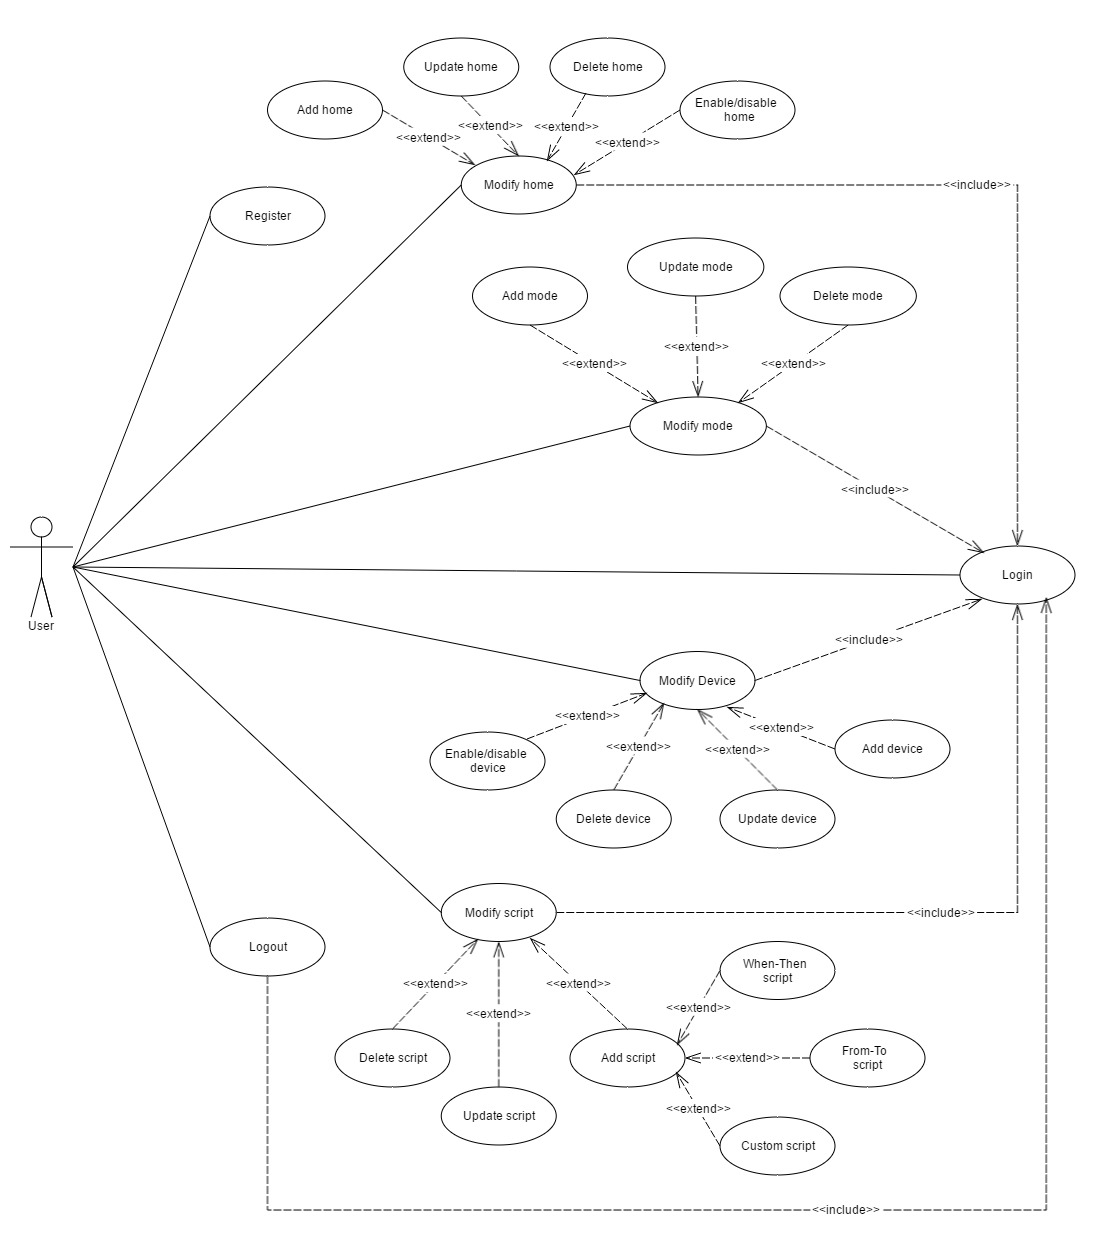
\includegraphics[width=15.5cm]{2-Usecase}
  \caption{Sơ đồ usecase của hệ thống}\label{fig:2-Usecase}
\end{figure}

\noindent
\textbf{Đăng ký (Register):} Chức năng đăng ký cho phép người dùng đăng ký một tài khoản để có thể sử dụng hệ thống. Người dùng cần nhập những thông tin như họ tên, tên đăng nhập, địa chỉ, email và mật khẩu. Sau khi đã đăng ký xong, người dùng sẽ sử dụng tài khoản này đề đăng nhập và tiến hành tạo nhà, thêm các thiết bị, tạo kịch bản,\dots\\

\noindent
\textbf{Đăng nhập (Login):} Đăng nhập là bước bắt buộc để có thể sử dụng các dịch vụ của hệ thống. Người dùng cần nhập đúng tên đăng nhập và mật khẩu đã đăng ký, nếu thành công, hệ thống sẽ hiển thị danh sách các ngôn nhà có thể truy cập, nếu đăng nhập thất bại, hệ thống cần hiển thị thông báo lỗi để người sử dụng thử lại.\\

\noindent
\textbf{Chỉnh sửa nhà (Modify home):} Chỉnh sửa nhà bao gồm 3 thao tác con là thêm (add), cập nhật (update), xóa (delete) và kích hoạt/vô hiệu hóa (enable/disable). Khi một người sử dụng hệ thống lần đầu vừa hoàn tất việc đăng ký và đăng nhập thành công vào hệ thống, điều đầu tiên họ cần làm là tiến hành tạo nhà. Khi tạo nhà, người dùng cần nhập các thông tin cần thiết như tên nhà, địa chỉ, …Do một người có thể quản lý nhiều căn nhà nên người sử dụng có thể tạo nhiều nhà khác nhau. Sau khi tạo, nếu cảm thấy có sai sót, người dùng có thể cập nhật lại thông tin của ngôi nhà đó, hoặc nếu không còn quản lý một ngôi nhà nữa, người dùng có thể tiến hành xóa ngôi nhà đó ra khỏi danh sách những ngôi nhà đang được quản lý của mình. Nếu muốn hệ thống trong nhà ngừng hoạt động trong một khoảng thời gian nhất định, người dùng có thể sử dụng chức năng vô hiệu hóa nhà (disable home), khi đó, tất cả các kịch bản (script) trong nhà sẽ dừng tạm thời. Nếu muốn trở lại bình thường, người dùng chỉ cần kích hoạt lại ngôi nhà (enable home).\\\\
\textbf{Chỉnh sửa chế độ (Modify mode):} Một ngôi nhà có nhiều chế độ (mode) khác nhau như chế độ vắng nhà, chế độ có nhà, chế độ đi chơi,\dots\hspace{0mm} Tại mỗi chế độ sẽ có những kịch bản khác nhau hoạt động, như ở chế độ có nhà, đèn cần được bật từ 18h tối đến 6h sáng, ngược lại, ở chế độ vắng nhà thì không cần bật đèn vào buổi tối mà cần kích hoạt cảm biến chuyển động được đặt trước cửa để chống trộm. Vì vậy, hệ thống cần cung cấp chức năng thêm chế độ (add mode) để người dùng có thể tạo ra những chế độ của riêng mình. Và hiển nhiên, hệ thống cũng cần cung cấp thêm tính năng cập nhật (update mode) và xóa (delete mode).\\\\
\textbf{Chỉnh sửa thiết bị (Modify device):} Sau khi đã tạo nhà, tạo chế độ cho một căn nhà, điều tiếp theo mà người sử dụng cần là thêm các thiết bị vào ngôi nhà của mình (add device). Chỉ sau khi thêm thiết bị thành công, người dùng mới có thể thêm kịch bản cho từng thiết bị của mình. Để thêm một thiết bị, người dùng cần nhập đầy đủ thông tin về thiết bị đó như tên thiết bị, loại thiết bị, mô tả,\dots\hspace{0mm} Bên cạnh đó, hệ thống cần cung cấp chức năng cập nhật thông tin thiết bị (update device) và xóa (delete device) nếu người dùng cảm thấy thiết bị đó không còn được dùng nữa. Hệ thống cũng cần cung cấp chức năng vô hiệu hóa thiết bị (disable device) trong những trường hợp người dùng muốn dừng các kịch bản đang hoạt động trên thiết bị này một cách tạm thời, sau đó, người dùng có thể kích hoạt lên lại bất kỳ khi nào họ muốn (enable device).\\

\noindent
\textbf{Chỉnh sửa kịch bản (Modify script):} Để thiết bị hoạt động theo một kịch bản được xác định trước, hệ thống cung cấp cho người dùng chức năng thêm kịch bản (add script). Có ba loại kịch bản chính: kịch bản When-Then (When-Then script), kịch bản From-To (From-To script) và kịch bản tùy chỉnh (Custom script). Người dùng có thể truy cập vào từng thiết bị và thêm những kịch bản mà mình mong muốn. Sau khi thêm, người dùng có thể chỉnh sửa (update script) hoặc xóa (delete script) những kịch bản không sử dụng.
\\

\noindent
\textbf{Đăng xuất (Logout):} Sau khi hoàn tất phiên làm việc, người dùng có thể đăng xuất khỏi hệ thống. Điều này đảm bảo tài khoản người dùng được bảo mật, không bị sử dụng bởi những người dùng chung thiết bị. Sau khi đã đăng xuất, người dùng phải nhập lại tên đăng nhập và mật khẩu để truy cập lại vào ngôi nhà của mình.\\

\noindent
Với sơ đồ usecase đã trình bày, hệ thống đã đáp ứng được những yêu cầu cơ bản của một ứng dụng nhà thông minh như đăng nhập, tạo nhà, tạo chế độ, thiết bị, …Ngoài ra, hệ thống còn cung cấp chức năng thêm mới một kịch bản, đây là phần cốt lõi của ứng dụng, cho phép người dùng có thể tùy chỉnh cách hoạt động của các thiết bị trong nhà, tạo ra những kịch bản của riêng họ giống như lập trình cho một ngôi nhà.

\section{Tổng quan hệ thống}

\begin{figure}[h!]
  \centering
     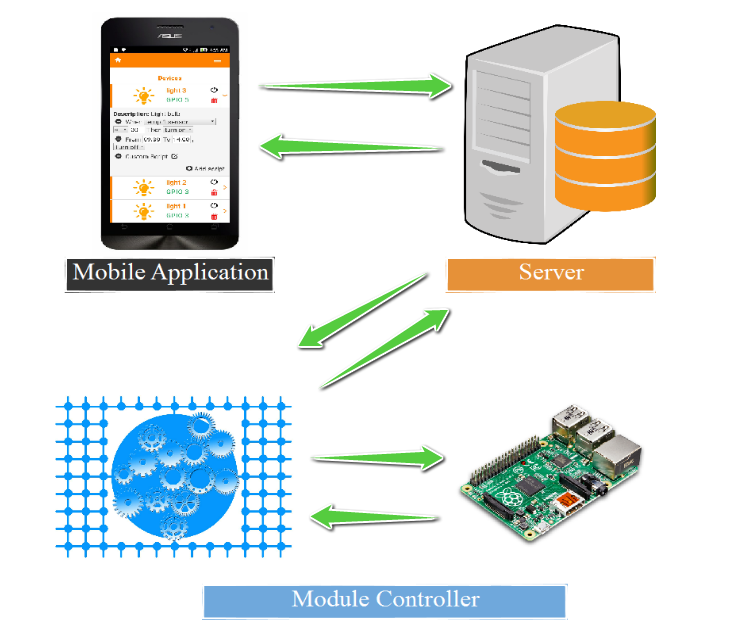
\includegraphics[width=12cm]{2-overview}
  \caption{Tổng quan hệ thống}\label{fig:2-overview}
\end{figure}

Để đáp ứng mục tiêu và yêu cầu đặt ra của đề tài về việc xây dựng hệ thống điều khiển các thiết bị thông dụng trong nhà thông qua các kịch bản, nhóm chúng tôi quyết định thiết kế hệ thống với 3 bộ phận chính: Module điều khiển thiết bị (Module Controller) đảm nhiệm việc kết nối và điều khiển các thiết bị được gắn với máy tính siêu nhỏ Raspberry Pi, máy chủ hệ thống (Server) với vai trò trung tâm xử lý các nghiệp vụ liên quan đến quản lý nhà, thiết bị, kịch bản trong hệ thống và ứng dụng di động (Mobile Application) cung cấp giao diện để người dùng truy cập và sử dụng hệ thống. Mối liên hệ của 3 bộ phận này được thể hiện ở hình \ref{fig:2-overview}.\\

\noindent
\textbf{Module điều khiển thiết bị (Module Controller):} Bộ phận này là một bộ điều khiển liên kết trực tiếp với máy tính siêu nhỏ Raspberry Pi nhằm gửi tín hiệu điều khiển đến các thiết bị phần cứng được kết nối cũng như nhận tín hiệu thông tin trả về từ các thiết bị này. Tùy vào chủng loại thiết bị phần cứng mà bộ điều khiển sẽ có cơ chế xử lý thông tin riêng. Module điều khiển thiết bị cung cấp API cho phía máy chủ hệ thống để máy chủ có thể gián tiếp truy cập, gửi nhận thông tin và điều khiển các thiết bị phần cứng một cách dễ dàng.\\

\noindent
\textbf{Máy chủ hệ thống (Server):} Bộ phận trung tâm của hệ thống, thông qua cơ sở dữ liệu xử lý các thao tác nghiệp vụ cốt lõi thêm mới, xóa, sửa các thông tin nhà, thiết bị, chế độ và vận hành các kịch bản của người dùng tạo ra. Từ đó, bộ phận này cung cấp một danh sách API để giao tiếp, truyền nhận thông tin với phía ứng dụng di động.\\

\noindent
\textbf{Ứng dụng di động (Mobile Application):} Người dùng truy cập và sử dụng hệ thống thông qua bộ phận này. Các giao diện về đăng ký, đăng nhập vào hệ thống, xem thông tin và quản lý danh sách nhà, thiết bị, chế độ và kịch bản được bộ phận này cung cấp.\\

\noindent
Với 3 bộ phận như trên, hệ thống được chia tách thành các thành phần độc lập nhưng có mối liên hệ chặt chẽ với nhau nhằm xử lý từng yêu cầu riêng biệt cũng như để đạt được mục tiêu chung của đề tài. Chi tiết về thiết kế và hiện thực của từng bộ phận được trình bày tại các chương 3, 4, 5 và 6.

%-----------------------------------Server--------------------------------%
\chapter{Back-end}
Phần này chúng ta sẽ thảo luận về thiết kế cơ sở dữ liệu (database) cho ứng dụng. Tiếp đến, ta sẽ đi vào giới thiệu tổng quan về các công nghệ mà nhóm đã tìm kiếm và ứng dụng trong việc xây dựng hệ thống này. Cuối cùng, dựa trên những phân tích về yêu cầu hệ thống, nhóm đề xuất và thiết kế ra mô hình kiến trúc của back-end để đáp ứng các nhu cầu đó.

\section{Thiết kế cơ sở dữ liệu}

\begin{figure}[h]
  \centering
     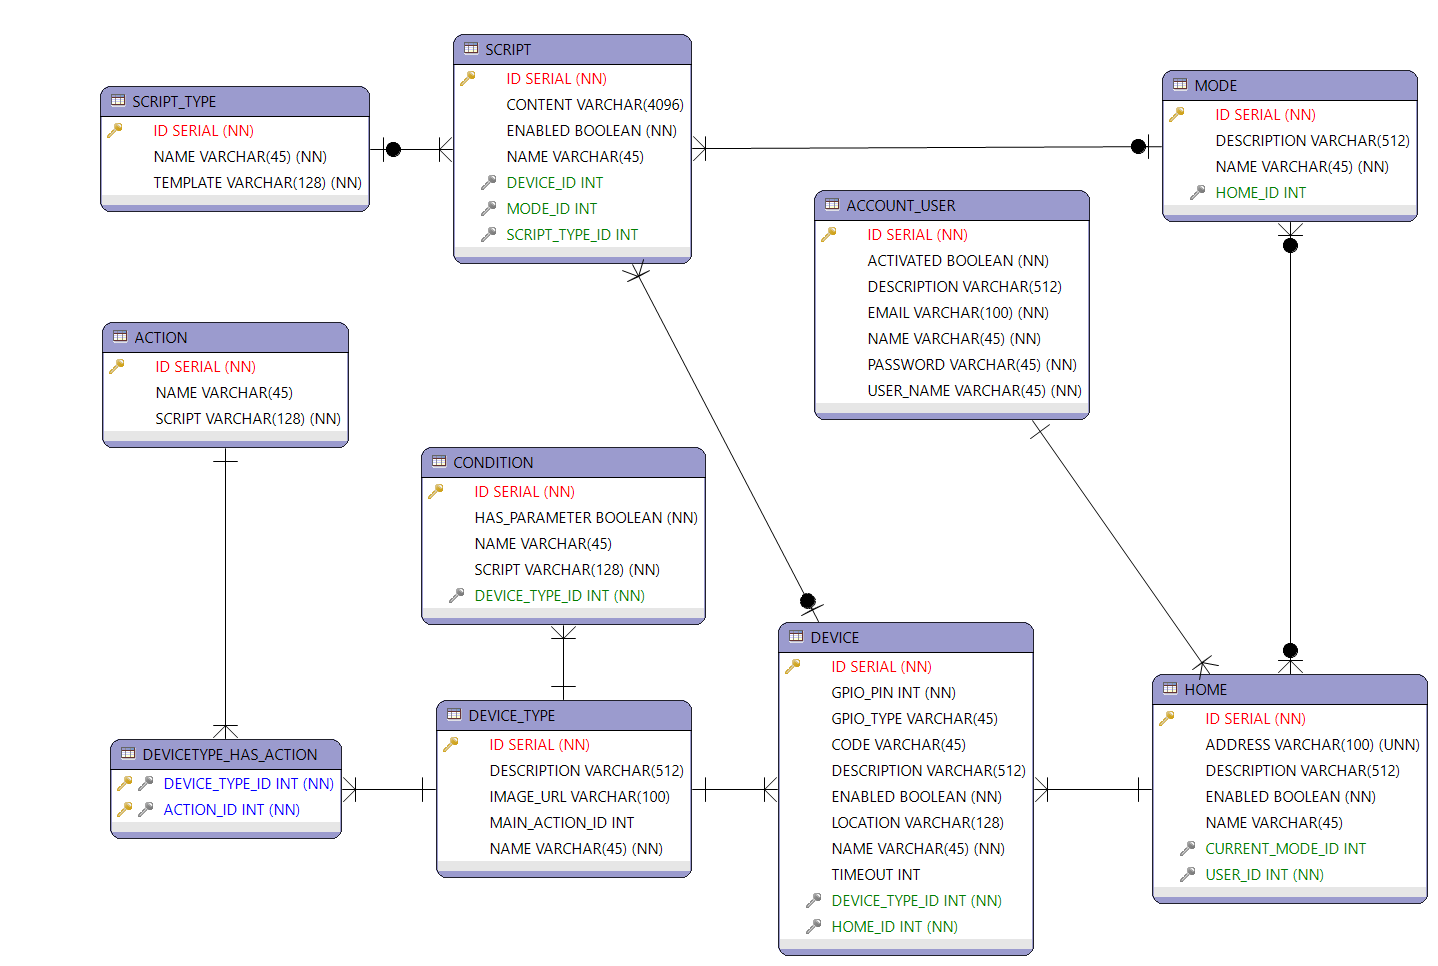
\includegraphics[width=15.5cm]{3-smart-home-db}
  \caption{Thiết kế database cho ứng dụng}\label{fig:3-smart-home-db}
\end{figure}

Mục tiêu của ứng dụng đó là tạo ra và lưu trữ các kịch bản của người dùng. Do đó, việc thiết kế database đóng một vai trò quan trọng trong việc xây dựng ứng dụng này. Ở phần thiết kế database, nhóm sử dụng PostgreSQL để hiện thực trên Raspberry Pi. Mô hình quan hệ giữa các bảng trong phần thiết kế database được trình bày như ở hình \ref{fig:3-smart-home-db}.\\

\noindent
Trở lại với yêu cầu được đặt ra từ hệ thống, người dùng có thể có nhiều ngôi nhà. Trong mỗi ngôi nhà sẽ điều khiển nhiều thiết bị khác nhau thuộc nhiều loại khác nhau. Mỗi thiết bị có thể có nhiều kịch bản để tự động hóa chúng. Kịch bản được đặc tả theo dạng \textbf{<điều kiện – hành động>}, nghĩa là dưới điều kiện nào đó do người dùng quyết định thì sẽ có những hành động tương ứng xảy ra. Những kịch bản sẽ hoặc thuộc dạng đơn giản (bao gồm 1 điều kiện, 1 hành động), hoặc dạng phức tạp mà người dùng có thể tự tạo theo ý muốn riêng của mình. Hơn nữa, với mỗi ngôi nhà có thể có nhiều chế độ quản lý nhưng tại 1 thời điểm chỉ có 1 chế độ được kích hoạt, ví dụ như chế độ đi vắng thì sẽ có những kịch bản riêng, còn với chế độ ở nhà sẽ là bộ kịch bản khác nhằm giúp người dùng tiện lợi trong việc quản lý căn nhà của mình ở nhiều hoàn cảnh khác nhau.\\

\noindent
Với cách thiết kế như trên, hệ thống có những đặc điểm

\begin{itemize}[topsep=1mm,itemsep=-0.5mm]
\item Tính thích ứng cao khi có thay đổi yêu cầu.
\item Đơn giản trong việc bảo trì và cập nhật (ví dụ như thêm thiết bị hay loại thiết bị mới).
\vspace{1mm}
\end{itemize}

\noindent
Chi tiết về chức năng các bảng trong thiết kế được mô tả ở bảng \ref{tab:db-tables}. Các bảng quan trọng trong hệ thống có thể kể đến là Account\_User, Home, Mode, Device, Script dùng để chứa dữ liệu của người dùng. Còn những bảng còn lại chủ yếu chứa dữ liệu của hệ thống (master data).

\begin{table}[h]
\centering
\caption{Chi tiết về chức năng các bảng được thiết kế trong database ứng dụng}\label{tab:db-tables}
\begin{tabular}{ |l|l|p{10cm}| } 
 \hline
	STT &	Tên bảng &	Chức năng\\ \hline
	1 &	Account\_User &	Thông tin liên quan đến tài khoản người dùng, đã kích hoạt hay chưa, một vài thông tin cá nhân cơ bản\\ \hline
	2 &	Home &	Thông tin liên quan đến nhà , có đang “active” hay không, nhà đang ở chế độ nào\\ \hline
	3 &	Mode &	Thông tin liên quan chế độ được người dùng định nghĩa cho ngôi nhà của mình\\ \hline
	4 &	Device &	Thông tin các thiết bị cho từng nhà  mà hệ thống quản lý như cổng GPIO, có đang ”active” không,\dots\\ \hline
	5 &	Device\_Type &	Loại thiết bị hệ thống có thể quản lý như đèn , còi , cảm biến,\dots\\ \hline
	6 &	Script &	Quản lý các thông tin liên quan đến kịch bản, kịch bản người dùng được lưu xuống theo 1 cú pháp định sẵn\\ \hline
	7 &	Script\_Type &	Phân loại kịch bản đơn giản, được cung cấp sẵn hay phức tạp\\ \hline
	8 &	Condition &	Những điều kiện hợp lệ gắn với từng loại thiết bị để sử dụng khi định nghĩa kịch bản\\ \hline
	9 &	Action &	Những hành động hợp lệ gắn với từng loại thiết bị để sử dụng khi định nghĩa kịch bản\\ \hline
	10 &	Device\_Has\_Action &	Mô tả mối quan hệ giữa loại thiết bị và hành động của chúng\\
 \hline
\end{tabular}
\end{table}

\section{Thiết kế và kiến trúc hệ thống back-end}

Hệ thống back-end được hiện thực hoàn toàn dựa trên ngôn ngữ Java và tận dụng sức mạnh từ Spring, một trong những framework được sử dụng nhiều nhất trong Java EE framework.\\

\noindent
Spring có thể giúp chúng ta xây dựng ứng dụng một cách nhanh chóng, tốn ít thời gian để làm quen. Spring cho phép các thư viện bên ngoài (third party service) tích hợp vào ứng dụng dễ dàng. Ví dụ như ứng dụng ta có thể kết nối đến nhiều loại database khác nhau với chi phí thay đổi rất thấp hay 1 ứng dụng Spring MVC có thể chuyển thành dịch vụ cung cấp tài nguyên thông qua REST API. Một điểm cộng nữa cho Spring đó là các công nghệ front-end đều có thể làm việc cùng với nó. Với sự phổ biến của Spring trong cộng đồng phát triển ứng dụng Java nền web cùng nhiều đặc điểm nổi trội so với các frameworks khác như: Struts, Vaadin,\dots\hspace{0mm} nhóm đã chọn Spring để phát triển hệ thống back-end này. Phần \ref{spring} sẽ cho ta cái nhìn tỗng quan về Spring framework, cùng những tính năng, ưu điểm của nó.

\subsection{Spring framework}\label{spring}

Hai khái niệm chính của Spring framework core là “Dependency Injection - DI” và “Aspect Oriented Programming - AOP”. Spring framework được sử dụng như là ứng dụng java cơ bản để đạt được kỹ thuật “loose coupling” giữa các components khác nhau bằng cách sử dụng kỹ thuật DI và hỗ trợ việc thực hiện chéo những task vụ như logging, authentication,\dots\hspace{0mm} theo kỹ thuật AOP \cite{spring-questions}\cite{spring-home-page}.\\

\noindent
Spring framework cung cấp khá nhiều tính năng khác và số lượng lớn các module cho các mục đích cụ thể, ví dụ như web có Spring MVC, hỗ trợ security có Spring Security, tương tác với datababse có Spring JDBC, và nhiều thứ khác nữa. Ngoài ra, nó còn là một dự án open source với rất nhiều cộng đồng sử dụng, tài liệu tham khảo.

\begin{figure}[h]
  \centering
     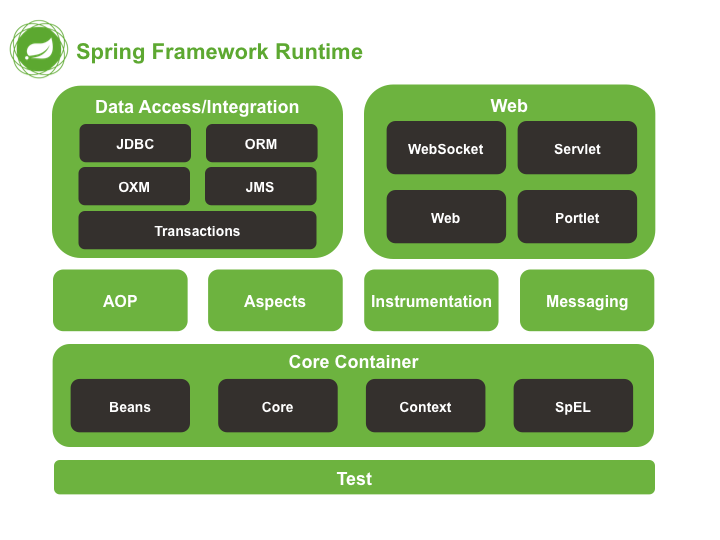
\includegraphics[width=12cm]{3-spring-framework-overview}
  \caption{Tổng quan về kiến trúc Spring Framework}\label{fig:3-spring-framework-overview}
\end{figure}

\noindent
Hình \ref{fig:3-spring-framework-overview} cho thấy kiến trúc tổng quan của Spring framework với nhiều module thiết kế tách biệt phục vụ cho nhiều mục đích khác nhau. Một số tính năng cũng như ưu điểm có thể kể đến của Spring:

\begin{itemize}[topsep=1mm,itemsep=-0.5mm]
\item Dependency Injection hoặc Inversion of Control được sử dụng để giúp các component tách rời, độc lập với nhau. Spring container sẽ giúp gắn kết những components này lại với nhau theo đặc tả business.
\item Spring MVC framework được sử dụng cho phát triển ứng dụng web rất dễ dàng với việc hỗ trợ rất tốt các tính năng web services, json,\dots\hspace{0mm}  (như RESTful web service framework).
\item Hỗ trợ quản lý transaction, JDBC operations, File uploading, Exception Handling,\dots\hspace{0mm} rất dễ dàng bằng cách cấu hình được rút gọn, thay vào đó là sử dụng annotation.
\item Làm giảm đi khối lượng code rất nhiều, chẳng hạn như việc khởi tạo đối tượng, open/close các resources,\dots
\vspace{1mm}
\end{itemize}

\noindent
Với đặc trưng của ứng dụng hiện tại là dùng những kịch bản quản lý tự động thiết bị trong nhà, không cần real time (như ứng dụng chat, stream video,\dots) và chỉ gửi yêu cầu tại một số thời điểm, với tần suất nhỏ nên nhóm lựa chọn dùng RESTful web service, xây dựng những API cho client có thể giao tiếp và truy xuất tài nguyên từ server một cách thuận tiện. Hơn thế nữa, tận dụng sức mạnh của Spring framework, việc xây dựng các RESTFul web service trở nên dễ dàng và tiết kiệm công sức hơn rất nhiều.

\subsection{RESTful Web Service}

Representational State Transfer (REST) là một kiểu kiến trúc được sử dụng trong việc giao tiếp giữa các máy tính (máy tính cá nhân và máy chủ của trang web) trong việc quản lý các tài nguyên trên internet. Hình \ref{fig:3-client-communicate-RESTfulWS} là sơ đồ thể hiện cách giao tiếp giữa client và máy chủ RESTFul web service thông qua giao thức HTTP \cite{restful-basic}.

\begin{figure}[h]
  \centering
     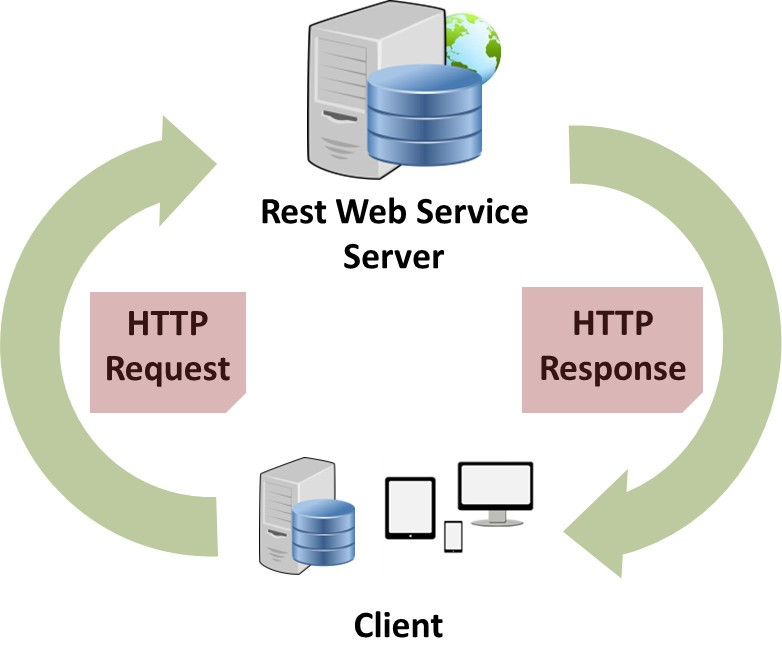
\includegraphics[width=7cm]{3-client-communicate-RESTfulWS}
  \caption{Sơ đồ giao tiếp giữa Client và máy chủ RESTFul Web Service}\label{fig:3-client-communicate-RESTfulWS}
\end{figure}

\noindent
Những nguyên tắc cơ bản của một RESTFul Web Service:

\begin{itemize}[topsep=1mm,itemsep=-0.5mm]
\item Sử dụng các phương thức HTTP một cách rõ ràng.
\item Phi trạng thái.
\item Hiển thị cấu trúc thư mục như URIs.
\vspace{1mm}
\end{itemize}

\subsubsection{Sử dụng các phương thức HTTP một cách rõ ràng}

Một đặc tính quan trọng của dịch Web service RESTful là sử dụng một cách rõ ràng các phương thức HTTP theo cách một giao thức được xác định bởi RFC 2616.\\

\noindent
REST yêu cầu các nhà phát triển sử dụng phương thức HTTP một cách rõ ràng theo cách tương thích với giao thức chuẩn. Nguyên lý thiết kế REST cơ bản này thiết lập một ánh xạ 1-1 giữa các hành động tạo, đọc, cập nhật và xoá (CRUD) các quá trình vận hành và các phương thức HTTP. Theo cách ánh xạ này thì:

\begin{itemize}[topsep=1mm,itemsep=-0.5mm]
\item Để tạo một tài nguyên trên máy chủ, ta cần sử dụng phương thức POST.
\item Để truy xuất một tài nguyên, ta sử dụng GET.
\item Để thay đổi trạng thái một tài nguyên hoặc để cập nhật nó, ta sử dụng PUT.
\item Để huỷ bỏ hoặc xoá một tài nguyên, ta sử dụng DELETE \cite{restful-basic}.
\vspace{1mm}
\end{itemize}

\subsubsection{Phi trạng thái}

Một yêu cầu hoàn chỉnh, độc lập không đòi hỏi máy chủ thu thập được bất kỳ ngữ cảnh hoặc trạng thái của ứng dụng nào trong lúc xử lý yêu cầu. Một ứng dụng (hoặc máy khách) Web service REST chứa ở phần đầu và phần thân trang HTTP của một yêu cầu tất cả các tham số, ngữ cảnh và dữ liệu cần thiết bởi thành phần bên ngoài máy chủ để đưa ra một phản hồi. Phi trạng thái theo nghĩa này nâng cao tính hiệu quả của dịch vụ Web, đơn giản hoá thiết kế và sự thi hành của các thành phần của máy chủ vì khi máy chủ không có trạng thái sẽ huỷ bỏ nhu cầu để đồng bộ hoá các mảng dữ liệu với một ứng dụng bên ngoài \cite{restful-basic}.

\subsubsection{Hiển thị cấu trúc thư mục như URIs}

Các địa chỉ Web service REST nên có tính hiện thực theo nghĩa rằng chúng dễ dàng đối với người dùng. Có thể nghĩ rằng một địa chỉ đường dẫn như là giao diện tự đóng gói mà đòi hỏi ít lý giải hay tham chiếu, nếu có, đối với một nhà phát triển để hiểu nó nhắm đến điểm gì và phân phối tài nguyên liên quan. Cuối cùng, cấu trúc của địa chỉ nên rõ ràng, có thể đoán được và dễ hiểu.
Một cách để đạt được mức độ sử dụng này là xác định cấu trúc thư mục giống URIs. Loại URI này có thứ bậc, có điểm khởi nguồn tại một đường dẫn đơn giản, và có nhánh đi ra là các nhánh phụ thể hiện các vùng chính của dịch vụ. Theo định nghĩa này, một URI không chỉ là một chuỗi bị cắt không giới hạn, mà còn là một cây với các nhánh chính và nhánh dọc nối nhau tại các nút. Ví dụ: \url{http://www.myservice.org/discussion/topics/{topic}}.\\

\noindent
Các địa chỉ URIs nên giữ nguyên để khi tài nguyên thay đổi hoặc khi tiến hành thay đổi dịch vụ, đường liên kết cũng sẽ giữ nguyên. Việc này cho phép đánh dấu lại vị trí đang đọc. Nó cũng rất quan trọng vì mối liên quan giữa các tài nguyên mà được mã hoá trong các địa chỉ được giữ nguyên độc lập với các mối liên quan đại diện khi chúng được lưu trữ \cite{restful-basic}.\\

\noindent
Với thiết kế database của nhóm, giữa các thực thể có mối quan hệ, liên kết với nhau chặt chẽ. Việc quản lý và thao tác với dữ liệu trực tiếp trên các database thường là công việc nặng nhọc và dễ phát sinh lỗi với các lập trình viên. Hibernate framework ra đời, giúp ta giải quyết những khó khăn trên. Ta có thể mô tả các đối tượng Java (Java objects) đại diện tương ứng cho mối quan hệ giữa các thực thể ở database và Hibernate sẽ làm công việc chuyển ánh xạ đó. Hibernate còn giúp quản lý cả kết nối (connection) với database, quản lý session,\dots\hspace{0mm} Với những ưu điểm đó, nhóm chọn Hibernate để đơn giản hóa việc quản lý, truy xuất dữ liệu từ database. Hơn nữa, Hibernate cũng nhận được sự hỗ trợ từ Spring không nhỏ, tiết kiệm chi phí thời gian lẫn công sức trong việc xây dựng hệ thống. Phần \ref{hibernate} sẽ giới thiệu tổng quan về kiến trúc cũng như tính năng, điểm mạnh của Hibernate.

\subsection{Hibernate Framework}\label{hibernate}

Hibernate Framework là một công cụ mã nguồn mở, dung lượng nhỏ (lightweight) và ORM (Object Relational Mapping) giúp đơn giản hóa việc phát triển ứng dụng Java để tương tác với cơ sở dữ liệu. Do Hibernate Framework là một ORM framework cho persistence layer nên khi phát triển ứng dụng, lập trình viên chỉ cần tập trung vào những layer khác (như tầng ứng dụng-business) mà không cần xem xét nhiều về persistence layer, dẫn đến tránh thao tác nhiều với database.\\

\noindent
Cấu trúc Hibernate được thể hiện qua hình \ref{fig:3-hibernate-architecture}. Hibernate sử dụng nhiều API của Java như JDBC, Java Transaction, Java Naming and Directory Interface. JDBC cho  phép bất kỳ cơ sở dữ liệu nào với một trình điều khiển JDBC đều được hỗ trợ bởi Hibernate.

\begin{figure}[h]
  \centering
     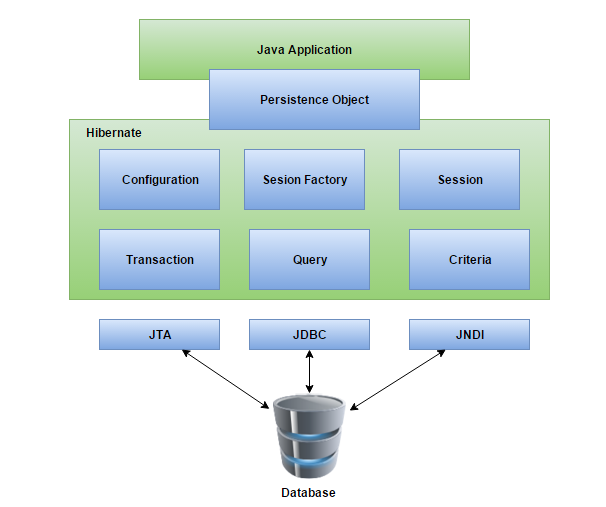
\includegraphics[width=12cm]{3-hibernate-architecture}
  \caption{Cấu trúc Hibernate}\label{fig:3-hibernate-architecture}
\end{figure}

\noindent
Dưới đây là một vài mô tả ngắn gọn về các thành phần trong cấu trúc Hibernate

\begin{itemize}[topsep=1mm,itemsep=-0.5mm]
\item Cấu hình đối tượng (Configuration): nó đại diện cho một tập tin cấu hình, cung cấp thông tin về database muốn kết nối đến. Đây cũng là thành phần tạo ra sự kết nối giữa các Java class và các bảng cơ sở dữ liệu.
\item SessionFactory: đối tượng này được tạo ra trong quá trình ứng dụng khởi động. Mỗi database sử dụng một tập tin cấu hình riêng biệt và chỉ có 1 đối tượng SessionFactory duy nhất. Đối tượng này có thể được truy cập đồng thời bởi nhiều thread nhưng vẫn đảm bảo tính an toàn dữ liệu (thread-safe).
\item Session: đối tượng này được ứng dụng dùng để giao tiếp với database. Các đối tượng Session không nên giữ mở trong thời gian dài vì không an toàn (not thread-safe).
\item Transaction: đối tượng này đại diện cho công việc nhỏ (ví dụ như cập nhật, lưu giá trị). Một session thường bao gồm nhiều transaction.
\item Query: đối tượng truy vấn sử dụng SQL hoặc Hibernate Query Language (HQL) để lấy dữ liệu từ cơ sở dữ liệu.
\item Criteria: kết hợp một hay nhiều tiêu chí để truy xuất một thực thể từ database thỏa mãn.
\vspace{1mm}
\end{itemize}

\noindent
Những lợi ích mà Hibernate đem lại

\begin{itemize}[topsep=1mm,itemsep=-0.5mm]
\item Hibernate Framework là mã nguồn mở theo LGPL licence và dung lượng nhỏ.
\item Đơn giản hóa việc truy nhập, kết nối
\item Hibernate Framework cung cấp các thiết bị để tạo ra các bảng tự động
\item Hỗ trợ hầu hết các loại database management system thông dụng hiện nay
\item Cung cấp cơ chế tự động quản lý cache, cache cấp 1 và cấp 2, giúp tối ưu hóa việc truy xuất dữ liệu.
\vspace{1mm}
\end{itemize}

\subsection{Kiến trúc back-end}

\begin{figure}[h]
  \centering
     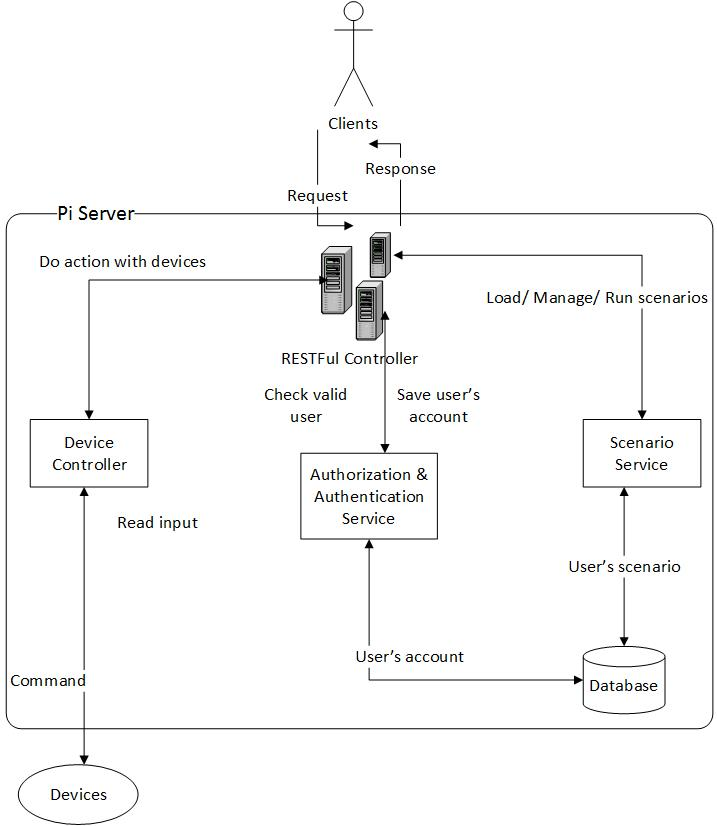
\includegraphics[width=15cm]{3-architecture-back-end}
  \caption{Kiến trúc hệ thống ở back-end}\label{fig:3-architecture-back-end}
\end{figure} 

\noindent
Hình \ref{fig:3-architecture-back-end} mô tả kiến trúc hệ thống ở back-end, bao gồm các module nhỏ như sau:

\begin{itemize}[topsep=1mm,itemsep=-0.5mm]
\item Authorization và Authentication service: phục vụ mục đích bảo mật hệ thống, chỉ những người dùng hợp lệ (có tài khoản hợp lệ, có quyền truy xuất với tài nguyên yêu cầu), quản lý token.
\item Scenario Service: quản lý trạng thái các kịch bản (có đang được kích hoạt chạy hay không) hay có thay đổi từ nhà hoặc thiết bị ảnh hưởng đến trạng thái kịch bản; quản lý việc thực thi các kịch bản một cách tự động; kiểm tra tính hợp lệ của kịch bản, xác định xem kịch bản có bị mâu thuẫn với chính nó hay với những kịch bản đã tồn tại hay không; cho phép truy xuất, tạo mới, cập nhật kịch bản.
\item Device Service: các kịch bản khi ở trong trạng thái kích hoạt và thỏa 1 điều kiện định trước do người dùng định nghĩa thì nó sẽ thực thi những hành động tương ứng. Và module này đóng vai trò trung gian trong việc tương tác với thiết bị thật gắn trên Raspberry Pi ở hệ thống back-end, cụ thể là các kịch bản đang chạy.
\vspace{1mm}
\end{itemize}

\noindent
Chi tiết về hiện thực các module này sẽ nằm trong mục \ref{back-end-implementation}

%-----------------------------------Device controller---------------------%
\chapter{Module điều khiển thiết bị}
Điều khiển các thiết bị điện trong nhà là một phần không thể thiếu trong hệ thống nhà thông minh. Server cần một bộ điều khiển có thể lấy được dữ liệu từ các cảm biến đặt tại các nơi khác nhau trong nhà, bật hoặc tắt các thiết bị điện,\dots\hspace{0mm} Trong chương này, chúng tôi đưa ra các công trình liên quan trong việc sử dụng máy tính siêu nhỏ Raspberry Pi để giải quyết nhiều vấn đề khác nhau trong cuộc sống. Tiếp đến, nhóm trình bày tổng quan thiết kế của module điều khiển thiết bị sử dụng Raspberry Pi và các công nghệ có thể hỗ trợ để hiện thực module.

\section{Tổng quan về Raspberry Pi}
Raspberry Pi được phát triển tại Anh bởi Raspberry Pi Foundation với mục đích giúp sinh viên có thể thực hành nhiều hơn trong môn Khoa học máy tính. Nó được thiết kế nhỏ gọn và phải đủ bền để sinh viên có thể giữ trong cặp. Hình \ref{fig:4-pi3-model-b} mô tả cấu trúc bên ngoài của máy tính Raspberry Pi 3 Model B \cite{pi-for-dummies}\cite{pi-wiki}.

\begin{figure}[h]
  \centering
     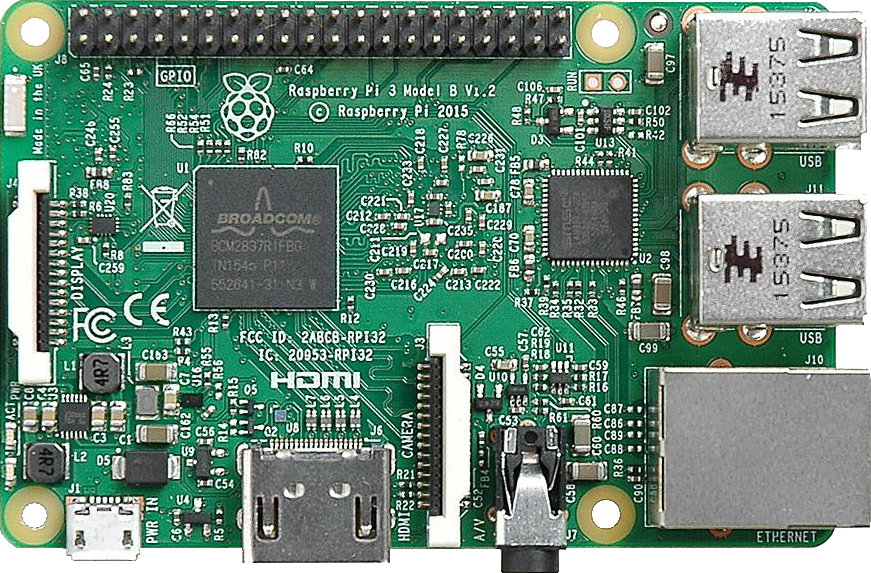
\includegraphics[scale=0.3]{4-pi3-model-b}
  \caption{Máy tính Raspberry Pi 3 Model B}\label{fig:4-pi3-model-b}
\end{figure}

\noindent
Giá thành của một con Raspberry Pi khá rẻ, phù hợp với túi tiền của tất cả mọi người. Trên thế giới, đã có rất nhiều sản phẩm hữu ích phục vụ cho đời sống và công việc hằng ngày ra đời nhờ sử dụng máy tính Raspberry Pi. Giáo sư Simon Cox và các đồng nghiệp đã lắp ghép 60 con Raspberry Pi bằng các viên gạch Lego để làm thành một chiếc siêu máy tính. Các máy tính Raspberry Pi này hoạt động song song với nhau và cùng giải quyết một vấn đề. Hình \ref{fig:4-Sieu-may-tinh} chụp lại hai trong số 60 con Raspberry Pi làm ra chiếc siêu máy tính \cite{pi-for-dummies}.

\begin{figure}[h]
  \centering
     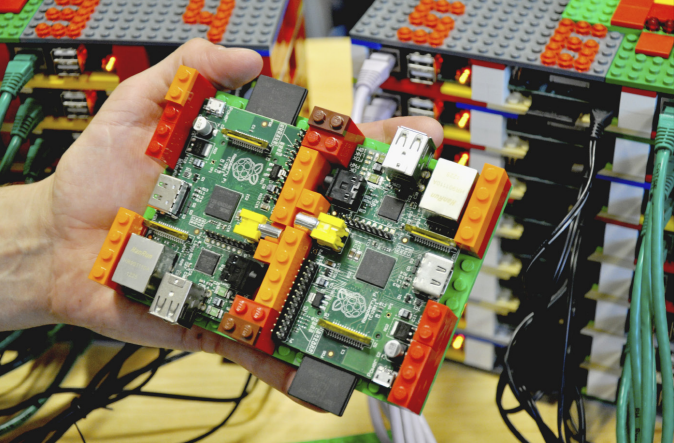
\includegraphics[scale=0.5]{4-Sieu-may-tinh}
  \caption{Siêu máy tính được chế tạo từ các con Raspberry Pi [2]}\label{fig:4-Sieu-may-tinh}
\end{figure}

\noindent
Một sở thú ở London, Anh cũng sử dụng Raspberry Pi để sáng tạo ra một công cụ gọi là EyesPi, cho phép chụp ảnh các hoạt động thường ngày của các loài động vật trong sở thú. Một người tên Dave Akerman đã cùng những người đồng nghiệp lắp đặt Raspberry Pi trên một khinh khí cầu, sau đó, họ thả bay khinh khí cầu và chụp những bức ảnh về Trái đất khi nhìn từ trên cao \cite{pi-for-dummies}.\\

\noindent
\textbf{Các phiên bản:} đã có nhiều thế hệ Raspberry Pi được đưa ra thị trường, phiên bản đầu tiên (Raspberry Pi 1 Model B) được ra mắt vào tháng 2 năm 2012. Từ năm 2012 cho đến nay đã có rất nhiều phiên bản Raspbery Pi ra đời với nhiều cải tiến. Raspberry Pi 3 Model B là phiên bản mới nhất tính đến thời điểm hiện tại, được phát hành vào tháng 2 năm 2016, tích hợp thêm bộ thu phát sóng WiFi và Bluetooth so với phiên bản trước. Đây cũng chính là phiên bản được nhóm lựa chọn sử dụng, thông số kỹ thuật được mô tả tại bảng \ref{tab:pi-3-model-b-specs} \cite{pi-wiki}.

\begin{table}
\centering
\caption{Một vài thông số kỹ thuật của Raspberry Pi 3 Model B}\label{tab:pi-3-model-b-specs}
\begin{tabular}{ |l|l| } 
 \hline
	Vi xử lý		&	ARMv8\\
	Xung nhịp		&	1.2GHz\\
	RAM				&	1 GB SDRAM\\
	Bộ nhớ trong	&	MicroSD\\
	Nguồn điện		&	5V\\
	GPIO			&	40 pin\\
	Video output	&	HDMI\\
	USB 2.0			&	4 cổng\\
	Cổng Ethernet	&	Có hỗ trợ\\
	Wireless		&	802.11n / Bluetooth 4.1\\
 \hline
\end{tabular}
\end{table}

\noindent
\textbf{Hệ điều hành:} Raspberry Pi đa phần sử dụng một hệ điều hành chuyên dụng là Raspbian. Đây là hệ điều hành mã nguồn mở, được xây dựng dựa trên nền tảng hệ điều hành Debian, được tạo ra bởi một nhóm nhỏ những người hâm mộ Raspberry Pi với mục đích tối ưu hóa cho việc sử dụng phần cứng của Raspberry Pi. Raspbian có khoảng 35000 packages cũng như những phần mềm biên dịch sẵn đính kèm, tiện cho việc cài đặt sử dụng \cite{pi-wiki}\cite{raspbian-front-page}.\\

\noindent
Ngoài hệ điều hành Raspbian, Raspberry Pi còn có thể chạy được Windows 10 IoT Core, một hệ điều hành được Microsoft thiết kế để sử dụng riêng cho hệ thống nhúng, và các hệ điều hành có nhân Linux khác như Ubuntu MATE, Xbian, CentOS,\dots\hspace{0mm} Trong quá trình phát triển ứng dụng, nhóm quyết định cài đặt hệ điều hành Raspbian trên Raspberry Pi vì đây vẫn là hệ điều hành được sử dụng và hỗ trợ nhiều nhất cho Raspberry Pi.

%--------------------------------------------------------------------------%
\section{Điều khiển thiết bị sử dụng GPIO}
Một trong những yếu tố quan trọng của Raspberry Pi là các cổng GPIO (General Purpose Input/Output) được bố trí dọc theo một cạnh của nó. Hình \ref{fig:4-vi-tri-dat-gpio} miêu tả vị trí đặt các cổng GPIO của Raspberry Pi 3 Model B \cite{raspberry-gpio}.

\begin{figure}[h]
  \centering
     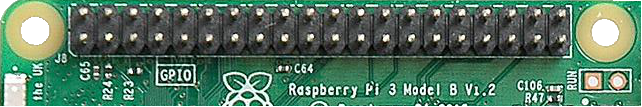
\includegraphics[scale=0.7]{4-vi-tri-dat-gpio}
  \caption{Vị trí đặt các cổng GPIO của Raspberry Pi 3 Model B}\label{fig:4-vi-tri-dat-gpio}
\end{figure}

\noindent
Mỗi cổng GPIO đều có hai trạng thái là High và Low tương ứng với mức điện áp lần lượt là 3.3V và 0V. Có thể xem các cổng GPIO như một cầu nối giữa Raspberry Pi và thế giới bên ngoài, mỗi cổng cũng có thể là input, cũng có thể là output cho tín hiệu số. Nói một cách đơn giản, mỗi cổng GPIO như một công tắc, người bên ngoài có thể tắt hoặc bật, tức thay đổi trạng thái cổng GPIO, lúc này, GPIO thực hiện chức năng là một cổng input. Các chương trình trên Raspberry Pi cũng có thể thay đổi trạng thái các cổng GPIO, GPIO lúc này thực hiện chức năng là một cổng output, truyền tín hiệu từ các trương trình ra ngoài \cite{raspberry-gpio}.\\

\noindent
Trong số 40 cổng của Raspberry Pi 3 Model B, có 26 cổng GPIO, 4 cổng nguồn có điện áp luôn luôn là 3.3V hoặc 5V, 8 cổng đất và 2 cổng ID EEPROM được dùng trong các mục đích đặt biệt. Trong số 26 cổng GPIO, một vài cổng có thêm những những chức năng khác ngoài việc thay đổi trạng thái giữa High và Low. Những cổng có thêm những chức năng đặc biệt này được gắn thêm một nhãn tên phía sau như mô tả trong hình \ref{fig:4-pi3-gpio}: 

\begin{figure}[h]
  \centering
     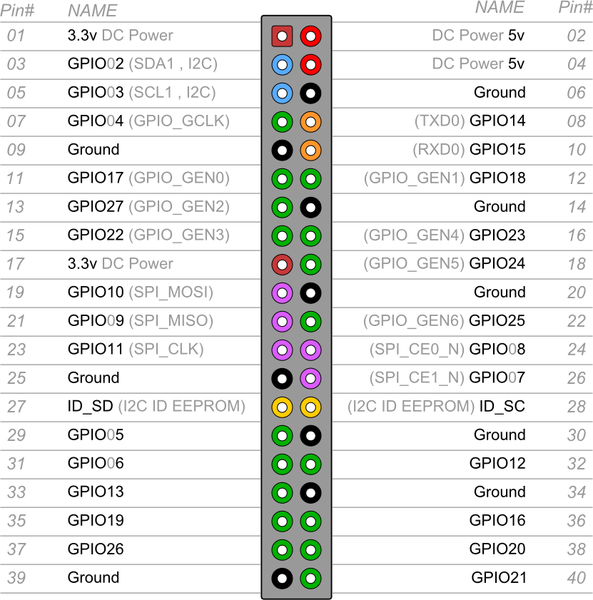
\includegraphics[width=11cm]{4-pi3-gpio}
  \caption{Vị trí phân bố các cổng GPIO}\label{fig:4-pi3-gpio}
\end{figure}

\begin{itemize}[topsep=1mm,itemsep=-0.5mm]
\item UART (Universal Asynchronous Receiver/Transmitter) Serial Bus: Giả sử như chúng ta cắm một thiết bị vào mà nó có khả năng hiển thị dữ liệu lên thì khi cắm vào hai chân này, ta có thể đọc được những thông báo từ kernel của Raspberry Pi. Ví dụ như Pi không thể khởi động lên được, ta dùng cách này như một công cụ chẩn đoán lỗi. Có hai GPIO hỗ trợ chức năng này là GPIO 15 và 16.

\item I2C (Inter - Integrated Circuit) Bus: cung cấp phương thức giao tiếp giữa nhiều ICs với nhau. Đối với Pi, một IC có thể nhắc đến ngay đó là mạch vi xử lý của nó. I2C bus có thể được truy cập từ GPIO 8 (SDA – Serial Data Line) và GPIO 9 (SCL - Serial Clock). Nó được dùng khá phổ biến để kết nối đến các thiết bị ngoại vi như cảm biến nhiệt độ hay màn hình LCD.

\item SPI (Serial Peripheral Interface) Bus: phục vụ cho in-system programming (ISP). Các GPIO sau hỗ trợ SPI : GPIO 10,11, 12, 13, 14.
\vspace{1mm}
\end{itemize}

%---------------------------------Thiết kế chi tiết-------------------------%
\section{Thiết kế chi tiết}

Vai trò chính của module điều khiển thiết bị là nhận yêu cầu từ server gửi đến và thực hiện đúng hành động mà server mong muốn. Để hiện thực chức năng này, các thiết bị được gắn trực tiếp vào một máy tính siêu nhỏ gọi là Raspberry Pi, mỗi thiết bị được điều khiển thông qua các chân cắm gọi là GPIO nằm dọc một cạnh của Raspberry Pi. Hình \ref{fig:4-module-dieu-khien-overview} mô tả sự tương tác giữa server, module điều khiển thiết bị và Raspberry Pi.

\begin{figure}[h]
  \centering
     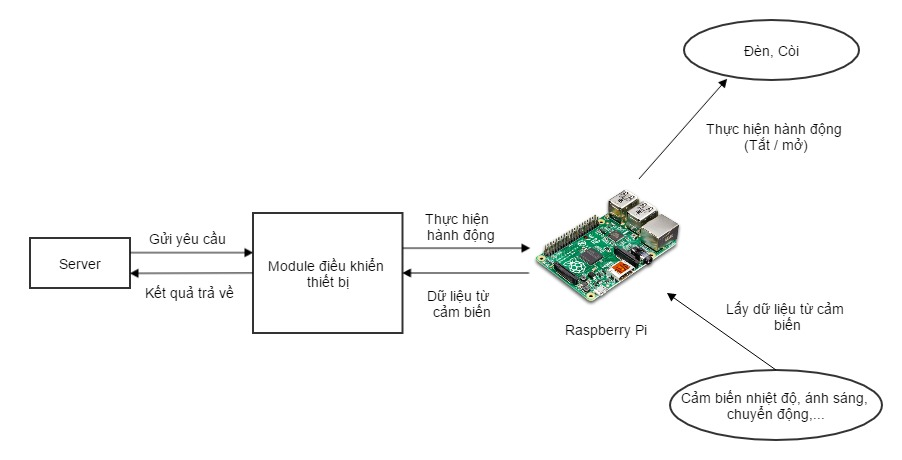
\includegraphics[scale=0.5]{4-module-dieu-khien-overview}
  \caption{Sơ đồ tổng quan của module điều khiển thiết bị}\label{fig:4-module-dieu-khien-overview}
\end{figure}

\noindent
Ví dụ, khi server muốn thực hiện hành động tắt đèn phòng khách, server sẽ gửi yêu cầu đến module điều khiển thiết bị kèm theo thông tin về thiết bị mà server cần điều khiển, trong trường hợp này là thông tin về chiếc đèn phòng khách. Trong những thông tin mà server gửi đến module điều khiển thiết bị thì số thứ tự cổng GPIO mà thiết bị này kết nối vào là thông tin quan trọng. Vì mỗi thiết bị sẽ được điều khiển bởi một GPIO, module điều khiển thiết bị cần biết chính xác chiếc đèn phòng khách được điều khiển bởi GPIO nào để thực hiện đúng hành động và đúng mục tiêu.\\

\noindent
Module điều khiển thiết bị được thiết kế gồm hai phần chính, được trình bày chi tiết tại hình \ref{fig:4-module-dieu-khien-detail}, bao gồm: bộ điều khiển tổng quát (General controller) và bộ cung cấp cổng GPIO (GPIO provider).

\begin{figure}[h]
  \centering
     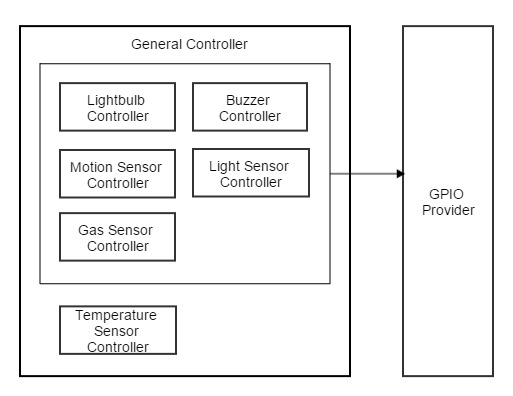
\includegraphics[scale=0.5]{4-module-dieu-khien-detail}
  \caption{Thiết kế chi tiết module điều khiển thiết bị}\label{fig:4-module-dieu-khien-detail}
\end{figure}

\noindent
\textbf{Bộ điều khiển tổng quát (General controller):} vai trò của bộ điều khiển tổng quát là nhận tất cả yêu cầu được gửi đến từ server và xử lý tất cả yêu cầu này, xác định xem đây là yêu cầu dành cho loại thiết bị nào và sử dụng đúng bộ điều khiển dành cho loại thiết bị đó. Trong bộ điều khiển tổng quát có chứa nhiều bộ điều khiển con dành cho từng loại thiết bị, tùy vào yêu cầu của server mà bộ điều khiển tổng quát sẽ quyết định sử dụng bộ điều khiển con nào. \\

\noindent
Bộ điều khiển đèn (Lightbulb controller) và bộ điều khiển còi (Buzzer controller) có vai trò như một công tắt đóng/mở. Mỗi thiết bị đèn hoặc còi sẽ được điều khiển bởi một cổng GPIO. Như đã trình bày, mỗi cổng GPIO đều có hai trạng thái là Low và High, tùy thuộc vào người thiết kế hệ thống mà từng trạng thái của GPIO sẽ tương ứng với bật hay tắt thiết bị. Trong dự dán của mình, nhóm sử dụng trạng thái Low là bật và trạng thái High là tắt.\\

\noindent
\textbf{Bộ cung cấp GPIO (GPIO provider):} bộ cung cấp GPIO có vai trò khai báo và cung cấp chính xác loại cổng mà bộ điều khiển thiết bị cần. Với các bộ điều khiển thiết bị dành cho cảm biến, bộ cung cấp GPIO cần khởi tạo cổng nhập (input pin) có chức năng nhận dữ liệu từ cảm biến. Đối với bộ điều khiển thiết bị cho đèn hoặc còi, bộ cung cấp GPIO cần khởi tạo cổng xuất (output pin) sử dụng cho việc điều khiển trạng thái bật/tắt.
%------------------------------------------------------------------------%

%--------------------------Công nghệ hỗ trợ---------------------------%
\section{Công nghệ hỗ trợ}
Có rất nhiều thư viện được viết bằng nhiều ngôn ngữ khác nhau hỗ trợ việc điều khiển các cổng GPIO của Raspberry Pi. Bên dưới là một vài công nghệ đang được sử dụng phổ biến hiện nay.\\

\noindent
\textbf{Thư viện Pi4J:} Pi4J là một thư viện được viết bằng ngôn ngữ Java với mục đích cung cấp các API (Application Programming Interface) cho người lập trình có thể điều khiển dễ dàng các cổng GPIO mà không cần quan tâm đến cấu trúc bên dưới của Raspberry Pi.\\

\noindent
\textbf{Thư viện WiringPi:} cũng là một thư viện được sử dụng để điều khiển các cổng GPIO, thư viện WiringPi được viết bằng ngôn ngữ C, là một thư viện hiệu quả đối với những chương trình viết bằng C hoặc C++. Tuy nhiên, đã có nhiều lập trình viên tạo thêm những phiên bản phù hợp với những loại ngôn ngữ khác như Java, Python, Ruby,\dots\\

\noindent
\textbf{Thư viện RPi.GPIO:} là một thư viện được viết bằng ngôn ngữ Python, RPi.GPIO được tạo ra với mục đích cung cấp những API cần thiết cho người lập trình Python có thể điều khiển các cổng GPIO của Raspberry Pi một cách dễ dàng.\\

\noindent
Sau khi tìm hiểu các công nghệ có thể hỗ trợ, chúng tôi quyết định chọn thư viện Pi4J sử dụng cho việc lấy dữ liệu và điều khiển trạng thái các cổng GPIO. Lý do nhóm quyết định lựa chọn thư viện này vì đây là thư viện mã nguồn mở, được công bố công khai tại GitHub. Vì vậy, nhóm có thể tùy chỉnh lại mã nguồn nếu cần thiết để tăng hiệu suất của hệ thống. Bên cạnh đó, phương pháp lập trình nhóm hướng đến là lập trình hướng đối tượng, nên chúng tôi ưu tiên sử dụng những thư viện được viết bằng ngôn ngữ Java.\\

\noindent
Với thiết kế của module điều khiển thiết bị đã được nêu ở những phần trên, tuy không thể điều khiển được tất cả các thiết bị có trong nhà, nhưng đủ để nhóm có thể tạo ra một mô hình thí nghiệm với đầy đủ các thiết bị cần thiết như các cảm biến, đèn và còi. Server được cung cấp đầy đủ các API để điều khiển tất cả các thiết bị hiện có phục vụ cho các mục đích khác nhau như bật/tắt đèn hoặc còi, lấy nhiệt độ, kiểm tra khí gas,\dots\hspace{0mm} Chi tiết hiện thực module điều khiển thiết bị sẽ được trình bày tại phần \ref{device-controller-implementation}.

%------------------------------------------------------------------------%

%-----------------------------------Mobile app-----------------------------%
\chapter{Ứng dụng di động}

Để có thể tương tác với hệ thống cũng như quản lý các thiết bị, kịch bản trong nhà thông minh, một ứng dụng di động với một giao diện đơn giản, dễ dùng dành cho người dùng là một điều tất yếu cần có. Trong chương này, chúng tôi sẽ giới thiệu tổng quan về các chức năng của ứng dụng di động, cũng như kiến trúc khái quát và các thành phần bên trong nó.

%--------------------------------Các chức năng của ứng dụng--------------%

\section{Các chức năng của ứng dụng}

Với mục tiêu hỗ trợ người dùng dễ dàng quản lý các ngôi nhà thông minh của mình, cùng với các thiết bị và kịch bản của ngôi nhà, ứng dụng di động được thiết kế để cho phép người dùng đăng ký và đăng nhập vào hệ thống, quản lý và chỉnh sửa thông tin các ngôi nhà được lắp đặt hệ thống và các thiết bị bên trong. Đồng thời, ứng dụng còn cho phép người dùng tạo ra nhiều chế độ khác nhau ứng với từng ngữ cảnh khác nhau (như vắng nhà, trời mưa, trời nóng…) với một bộ các kịch bản định sẵn hay tự tạo riêng biệt và chúng có thể được chuyển đổi qua lại một cách dễ dàng.

%-------------------------------------------------------------------------%
\section{Kiến trúc tổng quát}
Ứng dụng có kiến trúc bao gồm 6 trang giao diện (Page) chính là trang đăng nhập, trang đăng ký, trang danh sách các ngôi nhà, trang danh sách các kiểu thiết bị, trang danh sách các thiết bị và trang danh sách các kịch bản tự tạo. Trong mỗi trang có các bảng hộp thoại (Dialog) hỗ trợ người dùng thực hiện các chức năng của ứng dụng. Hình \ref{fig:5-UI-Flow} thể hiện luồng chạy và mối liên hệ giữ các trang và bảng hộp thoại trong ứng dụng.

\begin{figure}[h]
  \centering
     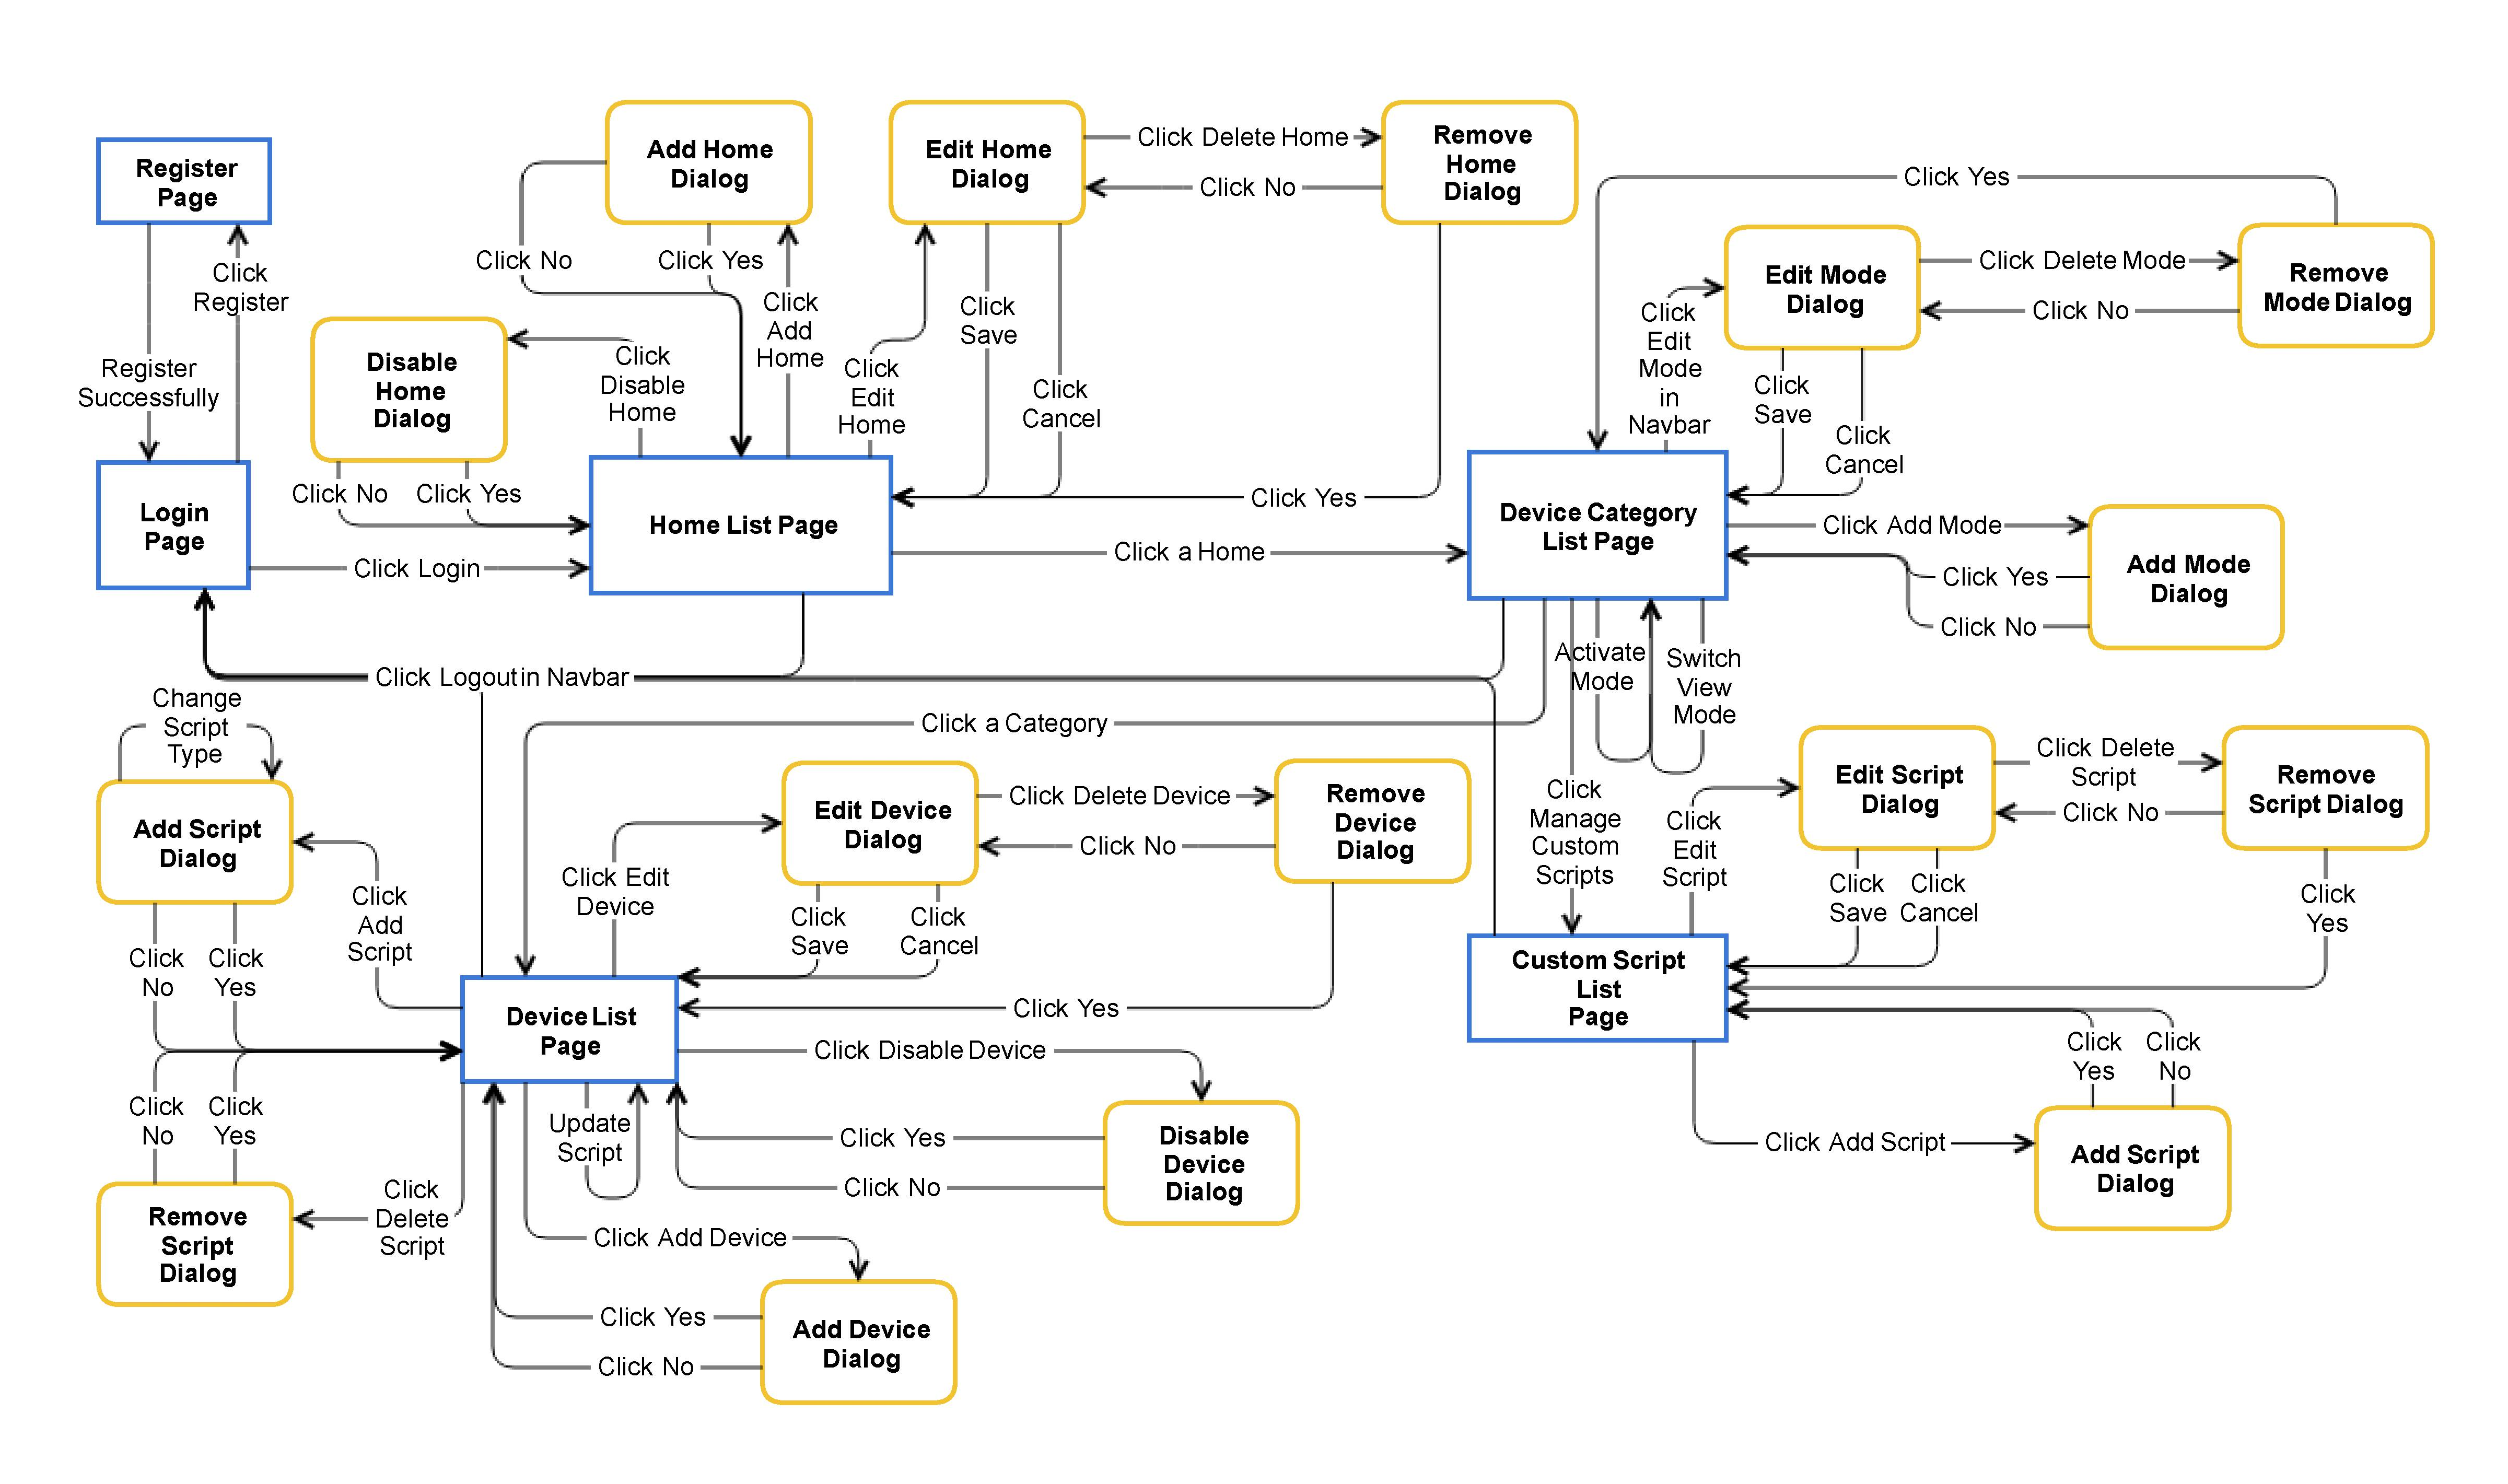
\includegraphics[width=16cm]{5-UI-Flow}
  \caption{Sơ đồ luồng Giao diện của ứng dụng di động}\label{fig:5-UI-Flow}
\end{figure}

\noindent
\textbf{Giao diện Đăng ký (Register Page):} Giao diện cho phép người dùng đăng ký tài khoản hệ thống với các thông tin là \textit{Tên đầy đủ}, \textit{Tên đăng nhập}, \textit{Mật khẩu}, \textit{Xác nhận mật khẩu} và \textit{Địa chỉ Email}. Sau khi người dùng nhập đầy đủ các thông tin và gửi lên hệ thống, một Email sẽ được gửi tới địa chỉ Email của người dùng để xác nhận các thông tin đăng ký. Giao diện này không có bảng hộp thoại nào. Từ giao diện này, người dùng có thể đến giao diện đăng nhập sau khi đã gửi thông tin đăng ký.\\

\noindent
\textbf{Giao diện Đăng nhập (Login Page):} Giao diện cho phép người dùng đăng nhập vào hệ thống với tên tài khoản và mật khẩu mà người dùng đã đăng ký. Giao diện này không có bảng hộp thoại nào. Từ giao diện này người dùng có thể đi đến giao diện đăng ký bằng cách nhấn nút đăng ký (Register) hoặc đến giao diện danh sách các ngôi nhà sau khi đã đăng nhập thành công.\\

\noindent
\textbf{Giao diện Danh sách các ngôi nhà (Home List Page):} Danh sách tên các ngôi nhà được lắp đặt hệ thống của người dùng được thể hiện ở Giao diện này. Với mỗi ngôi nhà, khi người dùng nhấn nút chỉnh sửa, bảng hộp thoại chỉnh sửa ngôi nhà sẽ hiện ra, tại đây người dùng có thể xem đầy đủ cũng như cập nhật lại thông tin của ngôi nhà, bao gồm \textit{Tên}, \textit{Địa chỉ} và \textit{Mô tả}. Để xóa một ngôi nhà, người dùng có thể nhấn nút xóa (Remove Home) tại bảng hộp thoại này, một bảng hộp thoại khác hiện lên yêu cầu người dùng xác nhận thao tác xóa. Để thêm mới một ngôi nhà, người dùng có thể nhấn nút thêm mới (Add Home) tại giao diện chính để mở bảng hộp thoại thêm mới yêu cầu người dùng nhập đầy đủ các thông tin về nhà mới. Ngoài ra, người dùng còn có thể dừng hoạt động của hệ thống hoặc cho phép hệ thống hoạt động trở lại tại mỗi ngôi nhà thông qua việc nhấn nút tắt/mở (Disable/Enable). Từ giao diện này, khi nhấn đăng xuất (Logout) từ thanh công cụ, người dùng sẽ về giao diện Đăng nhập hoặc khi nhấn vào một ngôi nhà, người dùng sẽ tới giao diện Danh sách các kiểu thiết bị.\\

\noindent
\textbf{Giao diện Danh sách các kiểu thiết bị (Device Category List Page):} Danh sách tên các kiểu thiết bị và danh sách tên các chế độ thuộc ngôi nhà được chọn sẽ được thể hiện ở Giao diện này. Tại đây, người dùng có thể chuyển đổi chế độ (Mode) thông qua hộp trình đơn thả xuống (Dropdown box) hoặc kích hoạt (Activate) một chế độ bất kì bằng cách nhấn vào tên chế độ đó tại thanh công cụ. Để chỉnh sửa thông tin hoặc xóa một chế độ nào đó, người dùng nhấn vào nút chỉnh sửa cạnh tên chế độ đó tại thanh công cụ. Để thêm mới một chế độ, người dùng có thể nhấn nút thêm mới (Add Mode) tại giao diện chính để mở bảng hộp thoại thêm mới yêu cầu người dùng nhập đầy đủ các thông tin về chế độ mới. Từ giao diện này, khi nhấn đăng xuất (Logout) từ thanh công cụ, người dùng sẽ về giao diện đăng nhập, khi nhấn vào một kiểu thiết bị, người dùng sẽ tới giao diện danh sách các thiết bị hoặc khi nhấn vào nút quản lý kịch bản tự tạo (Manage Custom Scripts), người dùng sẽ tới giao diện danh sách các kịch bản tự tạo.\\

\noindent
\textbf{Giao diện Danh sách các thiết bị (Device List Page):} Danh sách tên, chân GPIO các thiết bị thuộc kiểu thiết bị được chọn cũng như danh sách các kịch bản định sẵn thuộc chế độ được chọn của từng thiết bị được thể hiện ở giao diện này. Với mỗi thiết bị, khi người dùng nhấn nút chỉnh sửa, bảng hộp thoại chỉnh sửa thiết bị sẽ hiện ra, tại đây người dùng có thể xem đầy đủ cũng như cập nhật lại thông tin của thiết bị, bao gồm \textit{Tên}, \textit{Mô tả} và \textit{Vị trí}. Để xóa một thiết bị, người dùng có thể nhấn nút xóa (Remove Device) tại bảng hộp thoại này, một bảng hộp thoại khác hiện lên yêu cầu người dùng xác nhận thao tác xóa. Để thêm mới một thiết bị, người dùng có thể nhấn nút thêm mới (Add Device) tại giao diện chính để mở bảng hộp thoại thêm mới yêu cầu người dùng nhập đầy đủ các thông tin về thiết bị mới. Danh sách các kịch bản thuộc một thiết bị sẽ được thể hiện khi người dùng nhấn vào thiết bị đó, người dùng có thể xóa Kịch bản bằng cách nhấn nút xóa ở đầu mỗi kịch bản hoặc cập nhật lại thông tin kịch bản như \textit{Điều kiện}, \textit{Hành động} hay \textit{Thời gian bắt đầu}, \textit{Thời gian kết thúc} thông qua các hộp trình đơn thả xuống. Ngoài ra để thêm mới một kịch bản, người dùng có thể nhấn nút thêm mới Kịch bản (Add Script), bảng hộp thoại thêm mới kịch bản hiện ra, người dùng cần chọn loại kịch bản muốn thêm và xác định nội dung cho kịch bản đó. Từ giao diện này, khi nhấn đăng xuất (Logout) từ thanh công cụ, người dùng sẽ về giao diện đăng nhập hoặc khi nhấn vào biểu tượng ngôi nhà (Home) trên thanh công cụ, người dùng sẽ quay lại giao diện danh sách các kiểu thiết bị.\\

\noindent
\textbf{Giao diện Danh sách các Kịch bản tự tạo (Custom Script List Page):} Danh sách tên các kịch bản người dùng tự tạo thuộc chế độ được chọn sẽ được thể hiện ở giao diện này. Với mỗi kịch bản tự tạo, khi người dùng nhấn nút chỉnh sửa, bảng hộp thoại chỉnh sửa kịch bản tự tạo sẽ hiện ra, tại đây người dùng có thể xem cũng như cập nhật lại nội dung và tên của kịch bản. Để thêm mới một kịch bản tự tạo, người dùng có thể nhấn nút thêm mới kịch bản tự tạo (Add Custom Script), bảng hộp thoại thêm mới kịch bản tự tạo hiện ra yêu cầu người dùng xác định tên và nội dung cho kịch bản mới. Từ giao diện này, khi nhấn đăng xuất (Logout) từ thanh công cụ, người dùng sẽ về giao diện đăng nhập hoặc khi nhấn vào biểu tượng ngôi nhà (Home) trên thanh công cụ, người dùng sẽ quay lại giao diện danh sách các kiểu thiết bị.\\

\noindent
Với cách thiết kế như trên, kiến trúc ứng dụng di động cung cấp một giao diện tương đối đơn giản nhưng vẫn đáp ứng được các nhu cầu cơ bản về việc quản lý các ngôi nhà, thiết bị, chế độ và các kịch bản điều khiển thiết bị của người dùng.

%-----------------------------------Hiện thực và đánh giá------------------%
\chapter{Hiện thực hệ thống}

\section{Hiện thực back-end}\label{back-end-implementation}

\subsection{RESTFul Web Service - Cách thức giao tiếp giữa client và server}

Như đã đề cập ở phần Thiết kế back-end, nhóm đã chọn dùng RESTful web service làm cách giao tiếp chính giữa client và server. Một tiện ích khi sử dụng Spring framework đó là nó có hỗ trợ sẵn @RestController (là 1 annotation hỗ trợ bởi Spring framework), đơn giản hóa việc tạo ra các RESTful web services.

\begin{figure}[h]
  \centering
     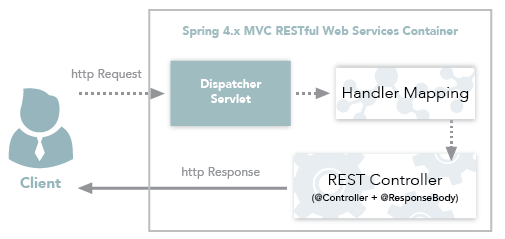
\includegraphics[width=12cm]{6-spring-RESTfulWS-workflow}
  \caption{Spring MVC RESTful Web services workflow}\label{fig:6-spring-RESTfulWS-workflow}
\end{figure} 

\noindent
Hình \ref{fig:6-spring-RESTfulWS-workflow} diễn tả luồng thực thi của Spring MVC REST, bao gồm các bước sau:

\begin{itemize}[topsep=1mm,itemsep=-0.5mm]
\item Client gửi yêu cầu đến web service theo như một định dạng URI nào đó có sẵn và hợp lệ.
\item Yêu cầu đi qua Servlet Dispacher đầu tiên và nó sẽ tìm ra 1 controller phù hợp nhất để xử lý yêu cầu đó.
\item Yêu cầu sau khi được xử lý bởi controller sẽ được gửi trả về client dưới định dạng JSON \cite{rest-controller}.
\vspace{1mm}
\end{itemize}

\noindent
Danh sách API có thể được tham khảo thêm ở mục \textbf{Phụ lục}.

\subsection{Cách thức giao tiếp với database}
Như đã đề cập ở mục thiết kế hệ thống back-end bên trên, nhóm sử dụng Hibernate framework để hỗ trợ cho các thao tác liên quan đến database. Hibernate cung cấp sẵn các hàm giúp truy xuất, lưu, cập nhật, xóa thực thể liên quan. Hình \ref{fig:6-DAO-structure} thể hiện tầng thao tác dữ liệu (DAO) trong ứng dụng mà nhóm đã thiết kế và hiện thực.

\begin{figure}[h]
  \centering
    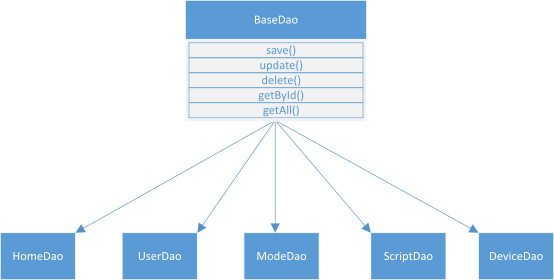
\includegraphics[width=12cm]{6-DAO-structure}
  \caption{ Tổ chức của tầng truy xuất dữ liệu (DAO)}\label{fig:6-DAO-structure}
\end{figure}

\noindent
Thiết kế này giúp tăng khả năng tái sử dụng (reuse), cũng như việc quản lý, bảo trì, mở rộng hệ thống được dễ dàng hơn trong tương lai. Ý tưởng cơ bản là có 1 class BaseDao, được hiện thực đầy đủ các hàm \textit{save}, \textit{update}, \textit{delete},\dots\hspace{0mm} còn các thực thể khác (như Home, User, Mode, Device, Script) thì thừa kế class BaseDao này và hiện thực thêm một số phương thức khác tùy theo nhu cầu.\\

\noindent
Nếu những thao tác với database gây ra lỗi, dữ liệu sẽ được rollback ngay thời điểm đó (ví dụ như vi phạm ràng buộc, khóa ngoại,\dots\hspace{0mm} ), nhằm đảm bảo tính nhất quán của dữ liệu.

\subsection{Giới thiệu về kịch bản (scenario)}

Kịch bản là một bản phác thảo, diễn tả những hành vi mình mong muốn thiết bị trong nhà sẽ tự động thực hiện trong hoàn cảnh nhất định hay điều kiện nào đó thỏa mãn. 

\subsubsection{Kịch bản người dùng}

Kịch bản người dùng sử dụng ngôn ngữ tự nhiên để đặc tả. Lấy ví dụ như “Trong khoảng thời gian từ 18h tối đến 22h tối thì bật đèn ở hành lang lên”. Vế đầu “trong khoảng thời gian từ 18h tối đến 22h tối” đặc tả điều kiện, vế sau “bật đèn hành lang” nêu ra hành động mong muốn khi mà điều kiện trên thỏa mãn.

\subsubsection{Kịch bản lưu trữ (script)}

Kịch bản lưu trữ có tác dụng như một bản thảo ngắn gọn của kịch bản người dùng, phục vụ mục đích lưu trữ dưới cơ sở dữ liệu là chính. Kịch bản lưu trữ được đặc tả bởi văn phạm riêng, được giới thiệu ở mục \ref{grammar} sắp tới.

\subsubsection{Kịch bản hệ thống (scenario)} 

Kịch bản hệ thống là dạng kịch bản mà hệ thống có khả năng “đọc”, “hiểu” và xử lý. Hệ thống đọc kịch bản lưu trữ và dùng 1 cấu trúc dữ liệu riêng (sẽ được giới thiệu ở mục \ref{grammar-data-structure}) để mô tả nó và xây dựng lên thành kịch bản hệ thống (lưu trên bộ nhớ máy tính).

\subsection{Văn phạm (grammar) dùng tạo ra kịch bản lưu trữ}\label{grammar}

Kịch bản của người dùng thường được đặc tả bởi ngôn ngữ tự nhiên. Với hệ thống hiện tại của nhóm, tính năng xử lý ngôn ngữ tự nhiên không được hỗ trợ, do đó vấn đề cấp thiết đặt ra đầu tiên và cũng không kém phần quan trọng, chính là đặc tả văn phạm cho kịch bản. Đặc tả văn phạm kịch bản nhằm một mặt giúp hệ thống có thể lưu trữ, mặt khác là phân định được kịch bản nào là hợp lệ và kịch bản nào không hợp lệ. Hơn thế nữa, văn phạm còn giúp hệ thống có thể “đọc”, “hiểu” và xử lý kịch bản. Tuy nhiên, công việc khó khăn là làm sao văn phạm đặc tả chính xác được kịch bản mà vẫn giữ đúng ý nghĩa của nó. Sau thời gian nghiên cứu, nhóm quyết định chọn BNF (Backus-Naur form), gồm những kí hiệu toán học để đặc tả văn phạm cho ngôn ngữ phi ngữ cảnh, thường dùng để xây dựng cú pháp các ngôn ngữ trong ngành máy tính, ví dụ như ngôn ngữ lập trình, tập lệnh\dots\hspace{0mm} áp dụng vào việc xây dựng văn phạm kịch bản hệ thống.\\

\noindent
Hình \ref{fig:6-system-grammar}  là mô tả văn phạm mà nhóm dùng để mô tả những kịch bản lưu trữ, bao gồm từ khóa (đặt trong cặp ngoặc kép), kí hiệu, phép toán, cấu trúc (đặt trong <>).

\begin{figure}[h!]
  \centering
    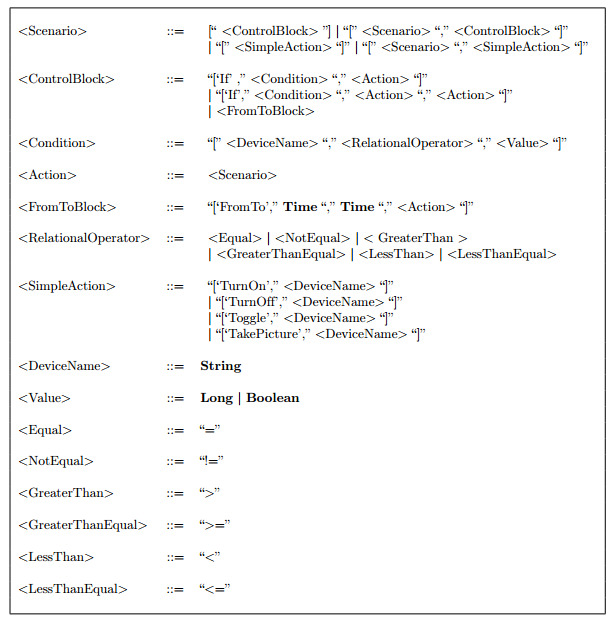
\includegraphics[width=16cm]{6-system-grammar}
  \caption{Văn phạm kịch bản lưu trữ}\label{fig:6-system-grammar}
\end{figure}

%\begin{table}[h]
%\centering\label{tab:grammars}
%\footnotesize
%\begin{tabular}[t]{ |lll| } 
%	\hline
%	&&\\
%	<Scenario>	&	::= & 
%	\begin{tabular}[t]{l}
%	[“ <ControlBlock> ”] | “[” <Scenario> “,”  <ControlBlock> “]” \\ 
%	| “[” <SimpleAction> “]” | “[” <Scenario>  “,”  <SimpleAction> “]”
%	\end{tabular}\\
%	
%	&&\\
%	<ControlBlock> 	&	::=	&
%	\begin{tabular}[t]{l}
%	“[‘If’ ,”  <Condition>  “,”  <Action> “]” \\
%	| “[‘If’,” <Condition> “,” <Action> “,” <Action> “]” \\
%	| <FromToBlock>
%	\end{tabular}\\
%	&&\\
%	
%	<Condition>  & ::= &
%	\begin{tabular}[t]{l}
%	“[” <DeviceName> “,”  <RelationalOperator> “,”  <Value> “]”
%	\end{tabular}\\
%	&&\\
%	
%	<Action> & ::= &
%	\begin{tabular}[t]{l}
%	<Scenario>
%	\end{tabular}\\
%	&&\\
%	
%	<FromToBlock> &	::= &
%	\begin{tabular}[t]{l}
%	“[‘FromTo’,”  \textbf{Time} “,” \textbf{Time} “,”  <Action>  “]” 
%	\end{tabular}\\
%	&&\\
%	
%	<RelationalOperator> &	::= &
%	\begin{tabular}[t]{l}
%	<Equal> | <NotEqual> | < GreaterThan > \\
%	| <GreaterThanEqual> | <LessThan> | <LessThanEqual> 
%	\end{tabular}\\
%	&&\\
%	
%	<SimpleAction> & ::= &
%	\begin{tabular}[t]{l}
%	“[‘TurnOn’,”  <DeviceName> “]”\\
%	| “[‘TurnOff’,”  <DeviceName> “]”\\
%	| “[‘Toggle’,” <DeviceName> “]”\\
%	| “[‘TakePicture’,”  <DeviceName> “]”
%	\end{tabular}\\
%	&&\\
%	
%	<DeviceName> & ::= & \textbf{String} \\
%	&&\\
%	
%	<Value> & ::= &	\textbf{Long} | \textbf{Boolean} \\
%	&&\\
%	
%	<Equal> & ::= &	“=” \\
%	&&\\
%	
%	<NotEqual> 	& ::= & “!=” \\
%	&&\\
%	
%	<GreaterThan> &	::= & “>” \\
%	&&\\
%	
%	<GreaterThanEqual> & ::= & “>=” \\
%	&&\\
%	
%	<LessThan> 	& ::= & “<” \\
%	&&\\
%	
%	<LessThanEqual>	& ::= & “<=”\\
%	&&\\
%	\hline
%\end{tabular}
%\end{table}

\noindent
Nhóm đã chọn đặc tả văn phạm kịch bản với cú pháp nêu trên, nhằm mục đích:
\begin{itemize}[topsep=1mm,itemsep=-0.5mm]
\item Có thể dễ dàng lưu trữ kịch bản.
\item Cú pháp tương tự như dạng JSON, nhóm có thể dùng parser JSON để phân tích và chuyển đổi thành kịch bản hệ thống dễ dàng hơn.
\vspace{1mm}
\end{itemize}

\noindent
Tuy nhiên, với cú pháp trên cũng có mặt hạn chế với cú pháp như việc tạo ra kịch bản lưu trữ cần phải được xử lý cẩn thận. Nếu khâu đầu vào có sai sót thì toàn bộ khâu còn lại, như đọc và xử lý sẽ gặp vấn đề. Để khắc phục hạn chế này, nhóm đã xây dựng 1 module nhằm tạo ra kịch bản hệ thống theo cú pháp nhất định (sẽ được giới thiệu trong mục \ref{script-builder}).\\

\noindent
Sau đây là một ví dụ trong thực tế về 1 kịch bản mà ta đang muốn hệ thống đọc, hiểu và xử lý:

\begin{itemize}[topsep=1mm,itemsep=-0.5mm]
\item “Nếu cảm biến nhiệt phát hiện nhiệt độ nằm trong khoảng 40 đến 50 độ C thì bật còi hú ở phòng khách”.
\item “Trong khoảng thời gian từ 18h tối đến 22h tối thì bật đèn ở hành lang lên”.
\vspace{1mm}
\end{itemize}

\noindent
Sử dụng văn phạm đã có, kịch bản lưu trữ dùng mô tả các kịch bản trên sẽ là:

\begin{itemize}[topsep=1mm,itemsep=-0.5mm]
\item \begin{verbatim}
“[ [‘If’, [‘temperature_sensor’,’>’, 40], 
[ [‘If’, [‘temperature_sensor’,’<’, 50], 
[ [‘TurnOn’, ‘buzzer_living_room’] ] ] ] ] ]”
\end{verbatim}
\item \begin{verbatim}
“[ [ ‘FromTo’, ’18:00’, ’20:00’, [ [ ‘TurnOn’, ‘light_lobby’ ] ] ] ]”
\end{verbatim}
\vspace{1mm}
\end{itemize}

\noindent
Với văn phạm đặc tả trên, hệ thống đã có thể phân định được kịch bản hợp lệ và không hợp lệ. Vì lý do thời gian nên nhóm chưa thể hỗ trợ nhiều dạng kịch bản hơn, nhưng việc mở rộng là hoàn toàn khả thi. Nhóm cũng đã liệt kê một số kịch bản thông dụng trên thực tế mà nhóm đã sưu tập và lặp nên (tham khảo thêm ở phần \textbf{Phụ lục}).

\subsection{Cấu trúc dữ liệu xây dựng kịch bản hệ thống}\label{grammar-data-structure}

\begin{figure}[h]
  \centering
    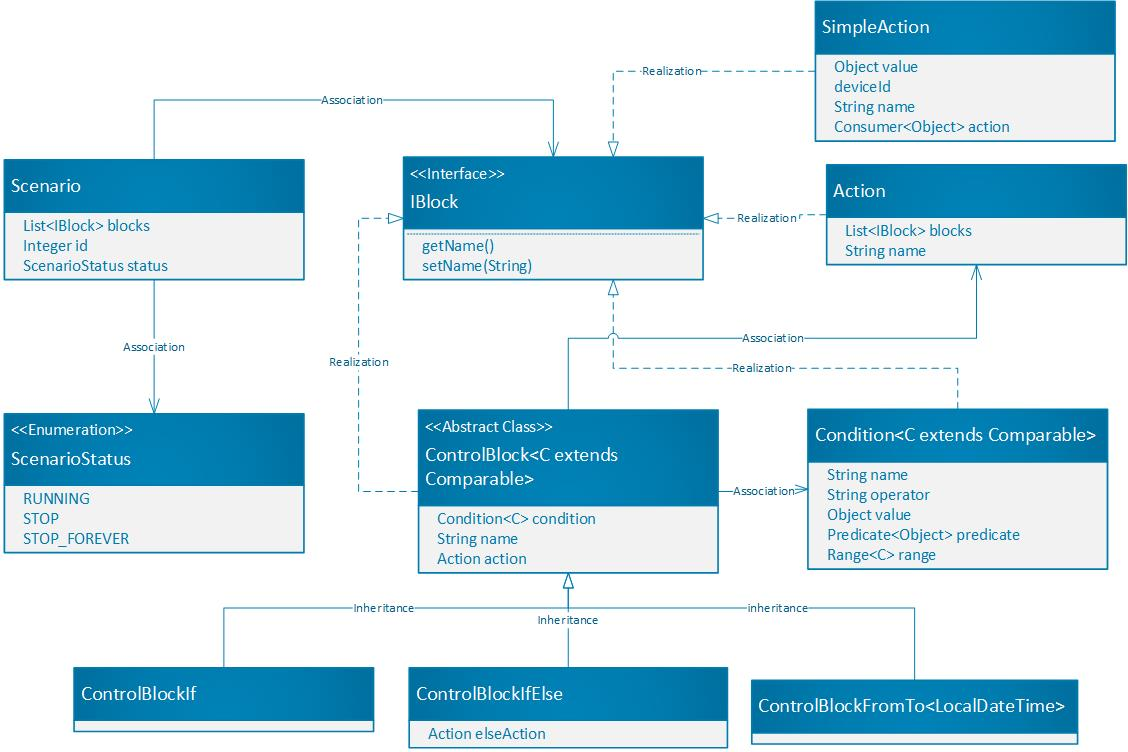
\includegraphics[width=15cm]{6-data-structure-scenario}
  \caption{Cấu trúc dữ liệu kịch bản hệ thống}\label{fig:6-data-structure-scenario}
\end{figure}

\noindent
Kịch bản hệ thống sẽ được lưu trữ trong bộ nhớ hệ thống khi chạy. Hình \ref{fig:6-data-structure-scenario} cho ta thấy cấu trúc dữ liệu của kịch bản hệ thống (scenario) bao gồm:

\begin{itemize}[topsep=1mm,itemsep=-0.5mm]
\item Thông tin trạng thái của nó, được định nghĩa bằng 1 enum ScenarioStatus là

	\begin{itemize}[topsep=1mm,itemsep=-0.5mm]
	\item RUNNING: đang được thực thi
	\item STOP: đã dừng lại (tạm thời và sau đó có thể được khởi động chạy lại)
	\item STOP\textunderscore FOREVER: dừng lại vĩnh viễn, trạng thái này dùng để kiểm soát những kịch bản trong hàng chờ được gỡ bỏ
	\vspace{1mm}
	\end{itemize}

\item Tập hợp các khối (block) hiện thực từ interface IBlock, các khối hợp lệ và được phép nằm trong kịch bản sẽ là

	\begin{itemize}[topsep=1mm,itemsep=-0.5mm]
	\item ControlBlock (sẽ chứa tham khảo đến Condition)
	\item Action
	\item SimpleAction
	\vspace{1mm}
	\end{itemize}
	
\vspace{1mm}
\end{itemize}

\subsubsection{Class SimpleAction}

Class SimpleAction đại diện cho những hành động nhỏ nhất, đơn giản nhất, có thể tương tác với thiết bị. Lấy ví dụ như hành động “Tắt đèn 1” hay “Bật còi hú ở bếp” là những hành động đơn giản.\\

\noindent
Thuộc tính “action” có kiểu Consumer<Object> nhằm để mình truyền vào 1 biểu thức dạng Lamda Expression, cụ thể nó là 1 hàm gọi tới Device controller, tương tác với thiết bị thật. Chi tiết về phần hiện thực sẽ được giải thích trong mục \ref{parser}.

\subsubsection{Class Action}

Class Action là tập hợp các hành động mong muốn thực hiện, có thể xem như là 1 kịch bản hệ thống “con” trong kịch bản hệ thống lớn bên ngoài và chứa nó. Vì thế mà cấu trúc của nó gần tương tự như là 1 kịch bản hệ thống vậy.

\subsubsection{Class Condition}

Class Condition dại diện cho 1 điều kiện nào đó. Lấy 1 ví dụ như “Nhiệt độ lớn hơn 40 độ C thì bật còi hú 1”. Phân tích kịch bản trên thì điều kiện ở đây chính là “Nhiệt độ lớn hơn 40 độ C”. Khi đó, thuộc tính “operator” sẽ có giá trị “>”, thuộc tính “value” có giá trị “40”. Một thuộc tính đặc biệt là range, kiểu Range<C> mang giá trị dãy số (40, +infinity), phục vụ cho mục đích kiểm tra kịch bản mâu thuẫn (giới thiệu ở phần \ref{script-validation}).\\

\noindent
Thuộc tính predicate có kiểu Predicate<Object> sẽ chứa 1 biểu thức Lamda Expression, tương ứng với điều kiện mà mình mô tả trong kịch bản. Chi tiết về hiện thực sẽ nằm trong mục \ref{parser}.

\subsubsection{Class ControlBlock và các class kế thừa từ nó}

Class ControlBlock được sinh ra nhằm mục địch kết nối 2 class: Action và Condition lại với nhau. Class ControlBlock này có 3 class kế thừa từ nó là

	\begin{itemize} [topsep=1mm,itemsep=-0.5mm]
	\item ControlBlockIf: ngữ nghĩa cơ bản là “Nếu điều kiện A xảy ra thì mình sẽ thực hiện hành động B”.
	\item ControlBlockIfElse: nó mang nghĩa “Nếu điều kiện A xảy ra thì mình sẽ thực hiện hành động B còn không thì sẽ thực hiện hành động C”. Vì thế mà nó có thêm 1 thuộc tính là “elseAction”, diễn tả hành động mong muốn được thực thi nếu mệnh đề điều kiện không thỏa mãn.
	\item ControlBlockFromTo: đây là khối điều khiển chuyên dụng cho các điều kiện liên quan tới thời gian, hiểu là “Trong khoảng thời gian từ X đến Y thì mình sẽ thực hiện hành động A”. Khoảng thời gian này có thể là trong cùng một ngày, hay kéo dài từ ngày này sang ngày tới. Ví dụ “Từ 18h00 đến 22h00 thì tắt đèn 1” hay “Từ 19h00 đến 01h00 sáng hôm sau thì bật đèn hành lang”.
	\vspace{1mm}
	\end{itemize}

\noindent
Nếu như sau này ứng dụng mở rộng và hỗ trợ thêm nhiều khối điều khiển khác, ta có thể kế thừa từ class ControlBlock này và tiếp tục hiện thực nó một cách dễ dàng.

\subsection{Sơ đồ mô tả luồng dữ liệu trong hệ thống khi thêm, sửa, xóa kịch bản người dùng}

\begin{figure}[h]
  \centering
    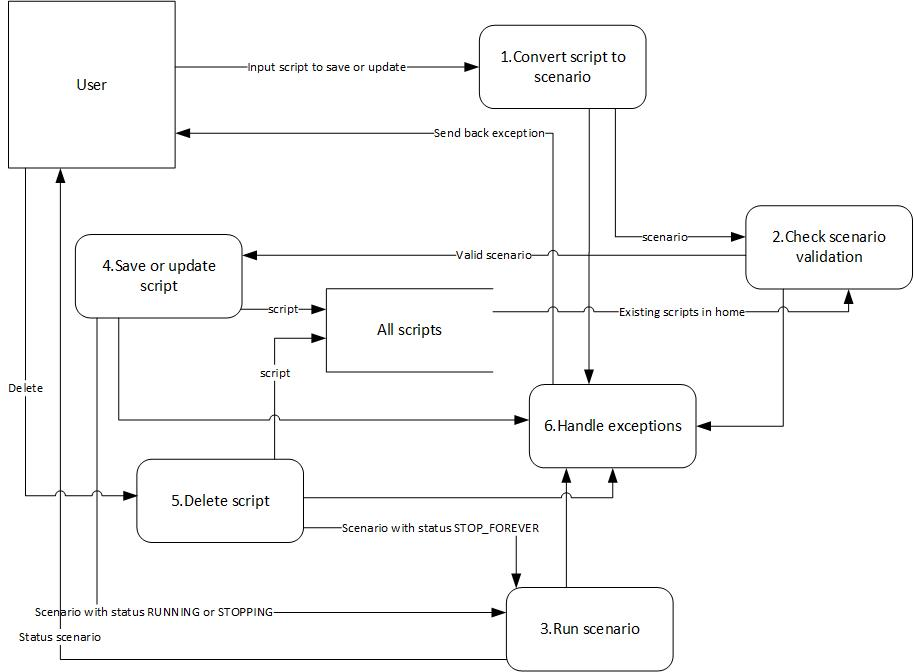
\includegraphics[width=15cm]{6-DFD-CRUD-action-with-script}
  \caption{Sơ đồ luồng dữ liệu khi thêm/sửa/xóa kịch bản}\label{fig:6-DFD-CRUD-action-with-script}
\end{figure}

\noindent
Một trong những chức năng chính của hệ thống đó là giúp người dùng quản lý thiết bị trong nhà một cách tự động, theo kịch bản được định sẵn. Hình 9 mô tả sơ đồ luồng dữ liệu của hệ thống back-end khi mà người dùng thêm, sửa hay xóa một kịch bản.\\

\noindent
Các tiến trình xử lý lần lượt theo các bước sau:

	\begin{itemize}[topsep=1mm,itemsep=-0.5mm]
	\item Khi người dùng thêm, sửa 1 kịch bản qua giao diện, phía client sẽ gửi về cho server thông tin kịch bản đó dưới dạng kịch bản lưu trữ.
	\item Kịch bản lưu trữ được chuyển đổi thành kịch bản hệ thống, được lưu trong bộ nhớ dưới 1 cấu trúc dữ liệu riêng bởi module \textbf{1.Convert script to scenario} (sẽ đi vào chi tiết ở mục module scenario creator). 
	\item Kịch bản hệ thống trên được kiểm tra tính hợp lệ, cũng như đảm bảo không mâu thuẫn (conflict) với những kịch bản khác hiện có trong ngôi nhà ấy bởi module \textbf{2.Check scenario validation} (sẽ đi vào chi tiết ở mục module Scenario Validation). Nếu như kịch bản không hợp lệ, thông báo lỗi sẽ được gửi trả về ngay cho người dùng.
	\item Sau khi kịch bản được kiểm tra tính hợp lệ, nó sẽ được lưu hay cập nhật vào cơ sở dữ liệu (mình sẽ lưu ở dạng kịch bản lưu trữ). 
	\item Việc cuối cùng là hệ thống sẽ “đọc” và xử lý kịch bản ấy. Việc quản lý đó được module \textbf{3.Run scenario} đảm nhiệm (sẽ đi vào chi tiết ở mục module Scenario Runner). Trạng thái của kịch bản mới sẽ được quyết định bởi người dùng, nó có thể là chưa được chạy (STOP) hay được chạy (RUNNING). Thông thường khi 1 kịch bản mới được thêm vào hệ thống sẽ mang trạng thái được chạy.
	\item Trong trường hợp mà người dùng muốn xóa một kịch bản, hệ thống back-end kiểm tra dưới cơ sở dữ liệu và gửi truy vấn xóa. Sau đó, hệ thống cập nhật lại trạng thái của kịch bản ấy là đã dừng vĩnh viễn (STOP\_FOREVER) và từ đó kịch bản này không còn có ảnh hưởng tới các thiết bị trong nhà nữa. 
	\vspace{1mm}
	\end{itemize}
	
\subsection{Module parser chuyển đổi kịch bản lưu trữ thành kịch bản hệ thống (scenario creator)}\label{parser}

Kịch bản lưu trữ chỉ phục vụ cho mục đích lưu dữ liệu. Khi hệ thống muốn đọc, hiểu, xử lý và chạy những kịch bản ấy thì nó cần được chuyển sang dạng kịch bản hệ thống. Để phục vụ cho nhu cầu đó, module scenario creator được sinh ra. Đầu vào của nó là một kịch bản lưu trữ và đầu ra sẽ là kịch bản hệ thống. Kịch bản hệ thống sẽ được dùng trong phần kiểm tra tính hợp lệ và chạy kịch bản như đã đề cập ở mục tổng quan phía trên.\\

\noindent
Kịch bản lưu trữ được thể hiện dưới dạng mảng JSON. Sở dĩ nhóm chọn cách thể hiện này là vì thư viện parse JSON đã có sẵn, việc tận dụng nó sẽ giúp giảm thời gian hiện thực hệ thống này. Mỗi một mảng JSON tương đương với 1 khối: điều kiện (condition) hay hành động (action) hay hành động đơn giản (simple action). Và cũng trong module này, nhóm đã áp dụng nhiều kĩ thuật mang tên Lamda Expression được hỗ trợ trong Java 8 để hiện thực việc xử lý 1 điều kiện hay là 1 hành động đơn giản tương tác với thiết bị thật.\\

\noindent
Khi xử lý 1 điều kiện, nhóm dùng Predicate class để hiện thực nó. Predicate như một mệnh đề luận lý trả về giá trị hoặc đúng, hoặc sai, rất phù hợp cho việc kiểm tra điều kiện. Một vài điều kiện cơ bản mà hệ thống hiện có đó là: kiểm tra xem đèn có được bật hay không, kiểm tra ngày hay đêm từ cảm biến ánh sáng, thực hiện so sánh nhiệt độ thu được từ cảm biến nhiệt với một giá trị người dùng mong muốn… Mỗi predicate sẽ nhận việc gọi đến device controller và kiểm tra giá trị trả về từ controller ấy. Nói cách khác thì khi hệ thống kiểm tra một điều kiện nào đó thì sẽ chỉ cần kiểm tra thuộc tính predicate bên trong cấu trúc kịch bản mà không phải gọi riêng lẽ một device controller nào. Nó giúp cho việc code được ngắn gọn và “sạch sẽ” hơn. Tương tự như việc xử lý 1 hành động đơn giản, nó có 1 thuộc tính “action” kiểu Consumer. Khi mà muốn thực hiện hành động, mình chỉ cần gọi phương thức trên biến “action” đó là đủ.

\subsection{Module hỗ trợ xây dựng kịch bản tùy ý (Script Builder)}\label{script-builder}

Hệ thống không chỉ cung cấp cho người dùng những kịch bản theo mẫu định sẵn, mà còn hỗ trợ cả kịch bản tùy biến. Để dễ dàng hơn cho người dùng định nghĩa 1 kịch bản tùy biến, nhóm tạo ra 1 module là Script Builder. Cú pháp của kịch bản người dùng tùy biến gần giống như ngôn ngữ tự nhiên, nhưng lại có khả năng chuyển đổi sang dạng kịch bản lưu trữ dễ dàng. Hình \ref{fig:6-user-grammar} mô tả cú pháp của văn phạm kịch bản tùy biến.

\begin{figure}[h!]
  \centering
     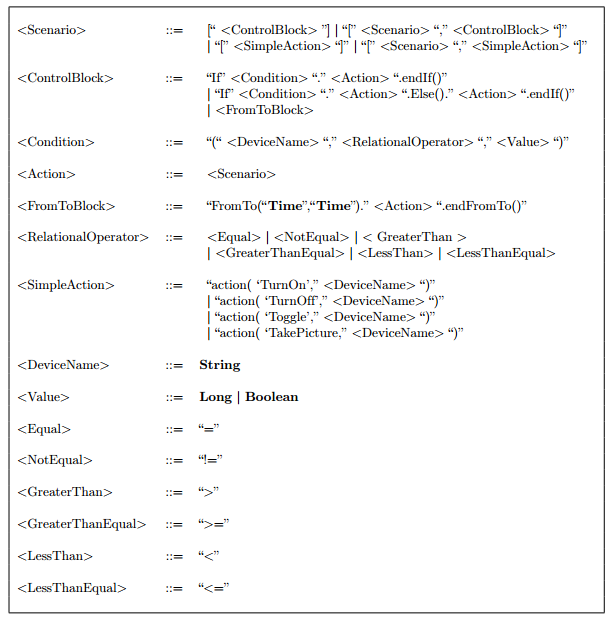
\includegraphics[width=16cm]{6-user-grammar}
  \caption{Văn phạm kịch bản tùy biến}\label{fig:6-user-grammar}
\end{figure}

\noindent
Lấy ví dụ về 1 kịch bản người dùng là: “Nếu nhiệt độ thu được từ cảm biến nhiệt gần cửa sổ lớn hơn 40 độ thì bật đèn phòng và bật đèn nhà bếp”.\\

\noindent
Kịch bản người dùng tùy biến được viết lại theo văn phạm trên sẽ là:
\begin{verbatim}
If(‘temp_sensor_near_window’, ‘>’ , ‘40’)
	.action(‘TurnOn’, ‘light_room’)
	.action(‘TurnOn’, ‘light_kitchen’)
.endIf()
\end{verbatim}

%\begin{table}[h]
%\centering\label{tab:user-grammars}
%\footnotesize
%\begin{tabular}[t]{ |lll| } 
%	\hline
%	&&\\
%	<Scenario>	&	::= & 
%	\begin{tabular}[t]{l}
%	[“ <ControlBlock> ”] | “[” <Scenario> “,”  <ControlBlock> “]” \\ 
%	| “[” <SimpleAction> “]” | “[” <Scenario>  “,”  <SimpleAction> “]”
%	\end{tabular}\\
%	&&\\
%	
%	<ControlBlock> 	&	::=	&
%	\begin{tabular}[t]{l}
%	“If”  <Condition> “.” <Action>  “.endIf()” \\
%	| “If”  <Condition>  “.”  <Action>  “.Else().”  <Action>  “.endIf()” \\
%	| <FromToBlock>
%	\end{tabular}\\
%	&&\\
%	
%	<Condition>  & ::= &
%	\begin{tabular}[t]{l}
%	“(“ <DeviceName>  “,” <RelationalOperator> “,” <Value> “)”
%	\end{tabular}\\
%	&&\\
%	
%	<Action> & ::= &
%	\begin{tabular}[t]{l}
%	<Scenario>
%	\end{tabular}\\
%	&&\\
%	
%	<FromToBlock> &	::= &
%	\begin{tabular}[t]{l}
%	“FromTo(“\textbf{Time}”,“\textbf{Time}”).”  <Action>  “.endFromTo()”
%	\end{tabular}\\
%	&&\\
%	
%	<RelationalOperator> &	::= &
%	\begin{tabular}[t]{l}
%	<Equal> | <NotEqual> | < GreaterThan > \\
%	| <GreaterThanEqual> | <LessThan> | <LessThanEqual> 
%	\end{tabular}\\
%	&&\\
%	
%	<SimpleAction> & ::= &
%	\begin{tabular}[t]{l}
%	“action( ‘TurnOn’,”  <DeviceName> “)”\\
%	| “action( ‘TurnOff’,”  <DeviceName> “)”\\
%	| “action( ‘Toggle’,”  <DeviceName> “)”\\
%	| “action( ‘TakePicture,”  <DeviceName> “)”
%	\end{tabular}\\
%	&&\\
%	
%	<DeviceName> & ::= & \textbf{String} \\
%	&&\\
%	
%	<Value> & ::= &	\textbf{Long} | \textbf{Boolean} \\
%	&&\\
%	
%	<Equal> & ::= &	“=” \\
%	&&\\
%	
%	<NotEqual> 	& ::= & “!=” \\
%	&&\\
%	
%	<GreaterThan> &	::= & “>” \\
%	&&\\
%	
%	<GreaterThanEqual> & ::= & “>=” \\
%	&&\\
%	
%	<LessThan> 	& ::= & “<” \\
%	&&\\
%	
%	<LessThanEqual>	& ::= & “<=”\\
%	&&\\
%	\hline
%\end{tabular}
%\end{table}
%

\noindent
Nhiệm vụ của client là sẽ mang kịch bản người dùng tùy biến trên gửi lên server, server sẽ dùng module ScriptBuilder để mà chuyển đổi sang kịch bản lưu trữ. Đi vào chi tiết module ScriptBuilder thì nó gồm 1 bộ biên dịch, nhằm thực thi một đoạn code được lưu dưới dạng chuỗi. Sở dĩ nhóm đề xuất văn phạm, cú pháp trên cho kịch bản tùy biến vì nó chính là đoạn code thu nhỏ, sử dụng ngôn ngữ Java. Nhiệm vụ của bộ biên dịch là đọc kịch bản đó giống như đọc và thực thi 1 đoạn code Java. Kết quả trả về từ đoạn code (hay kịch bản tùy biến) sẽ là một kịch bản lưu trữ. Bằng cách này, nhóm có thể cung cấp cho người dùng những cú pháp khác linh hoạt hơn và tiện lợi hơn (syntatic sugar), giúp người dùng định nghĩa một kịch bản tùy biến dễ dàng và thuận tiện nhất.\\

\noindent
Trước khi hiện thực module ScriptBuilder này, nhóm cũng đã tìm hiểu sơ qua các Rule Engine hỗ trợ xây dựng kịch bản. Theo tìm hiểu của nhóm, Rule Engine sẽ hỗ trợ cho ta định nghĩa ra các quy tắc cứng, đã được định nghĩa sẵn (thông thường là business rule) dành cho hệ thống trong một số trường hợp cụ thể nào đó. Khi ta muốn thay đổi các quy tắc ấy thì cần khởi chạy lại hệ thống để có hiệu lực. Chính vì thế mà Rule Engine không phù hợp với ứng dụng nhóm muốn phát triển. Có thể lý giải rằng các kịch bản người dùng đặt ra không phải là các business rule của hệ thống. Hơn nữa, những kịch bản ấy có tính linh hoạt, người dùng có thể cập nhật nội dung mới và nó tự động có hiệu lực ngay sau đó.

\subsection{Giới thiệu về tính hợp lệ của kịch bản và giải thuật kiểm tra tính hợp lệ}\label{script-validation}

\subsubsection{Thế nào là kịch bản tự mâu thuẫn (self-conflict script)}

Kịch bản tự mâu thuẫn là kịch bản chứa các điều kiện mâu thuẫn trong nội tại chính nó. Lấy ví dụ: Nếu như nhiệt độ thu được từ cảm biến nhiệt ở phòng khách lớn hơn 40 độ và bé hơn 30 độ thì bật đèn 1. Dễ dàng nhận thấy rằng 2 điều kiện “nhiệt độ lớn hơn 40 độ” và “nhiệt độ bé hơn 30 độ” mâu thuẫn lẫn nhau khi giá trị đó cùng thu thập được từ cùng 1 thiết bị. Vì thế, chúng ta có thể kết luận rằng kịch bản nêu trên là kịch bản tự mâu thuẫn. Nhưng nếu điều kiện nhiệt độ bé hơn 30 độ thu được từ 1 cảm biến nhiệt khác thì kịch bản trên không được gọi là tự mâu thuẫn.

\subsubsection{Thế nào là kịch bản mâu thuẫn (conflict) ?}\label{scenario-conflict}

Kịch bản này được gọi là mâu thuẫn với kịch bản kia nếu như cả 2 kịch bản có tồn tại 2 hành động đơn giản (simple action) trái ngược nhau (counter-action) nhưng điều kiện xảy ra hành động trên lại giống nhau. Hai hành động được gọi là trái ngược nhau nếu hành vi của chúng ngược với nhau và chúng cùng là hành động đơn giản (simple action). Lấy ví dụ, ta có 2 kịch bản sau

	\begin{itemize}[topsep=1mm,itemsep=-0.5mm]
	\item Kịch bản 1: Nếu đèn 1 bật thì đèn 2 tắt.
	\item Kịch bản 1: Nếu đèn 1 bật thì đèn 2 bật.
	\vspace{1mm}
	\end{itemize}

\noindent
Ta nhận thấy, 2 hành động “đèn 2 bật” và “đèn 2 tắt” là 2 hành động trái ngược nhau. Hơn nữa, điều kiện xảy ra hành động trái ngược nhau trên là “đèn 1 bật”. Có thể kết luận rằng 2 kịch bản trên là mâu thuẫn với nhau.

\subsubsection{Thế nào là kịch bản có khả năng mâu thuẫn (potential conflict)?}

Hai kịch bản được gọi là có khả năng mâu thuẫn nếu như giữa 2 kịch bản ấy tồn tại ít nhất một mâu thuẫn (theo khái niệm từ mục \ref{scenario-conflict}) và mâu thuẫn đó chỉ xảy ra trong một số điều kiện nhất định. Sau đây là ví dụ về kịch bản có khả năng mâu thuẫn.

	\begin{itemize}[topsep=1mm,itemsep=-0.5mm]
	\item Giả sử ta có kịch bản là “từ (12h40, 15h30) thì tắt đèn 1” và một kịch bản khác yêu cầu là bật đèn 1 nhưng có thời gian thực hiện không xác định (ví dụ: khi có gas, khi trời sáng, khi có người, khi nhiệt độ >, <,...). Hai kịch bản trên vẫn có khả năng mâu thuẫn vì giữa chúng tồn tại sự mâu thuẫn giữa hành động “bật” và “tắt” đèn 1 và thời gian thực hiện kịch bản thứ hai là không xác định, nó có thể là thời điểm nào đó trong ngày và cùng lúc điều kiện kịch bản 1 đang thực thi thì điều kiện kịch bản 2 cũng được thỏa mãn.
	\item Ví dụ như ta có kịch bản 1 là “Nếu nhiệt độ lớn hơn 35 độ và nếu đèn 1 tắt thì đèn 2 bật” và kịch bản 2 là “Nếu đèn 1 tắt thì đèn 2 tắt”. Ta nhận thấy ở kịch bản 1 có cặp <điều kiện, hành động> là <khi đèn 1 tắt, đèn 2 bật> mâu thuẫn với <khi đèn 1 tắt, đèn 2 tắt> ở kịch bản 2. Nhưng thực sự chỉ khi nhiệt độ lớn hơn 35 độ thì sự mâu thuẫn mới xảy ra, bình thường thì ta nói 2 kịch bản trên có khả năng mâu thuẫn mà thôi. 
	\item Trường hợp điều kiện cùng khoảng giá trị cũng là một dạng có khả năng mâu thuẫn. Lấy 1 ví dụ như “nhiệt độ trong khoảng (30,40) độ C thì thực hiện bật đèn 1” và “nhiệt độ trong khoảng (35,45) độ C thì tắt đèn 1”. Ta thấy là 2 khoảng giá trị trên có trùng lắp lẫn nhau và 2 hành động lại đối nghịch nhau. Hai kịch bản trên có khả năng mâu thuẫn.
	\item Hoặc trùng khoảng thời gian: tương tự như khoảng giá trị trên, còn bây giờ là khoảng thời gian. Ví dụ “từ (12h40, 15h30) thì bật đèn 1” và “từ (15h, 16h) tắt đèn 1” cũng là những kịch bản có khả năng mâu thuẫn.
	\vspace{1mm}
	\end{itemize}
	
\subsubsection{Định nghĩa về kịch bản hợp lệ}

Kịch bản hợp lệ là kịch bản không tự mâu thuẫn với chính nó, không trùng tên hay trùng nội dung hoàn toàn, không mâu thuẫn hay có khả năng mâu thuẫn với các kịch bản khác đã có ở cùng chế độ (mode) của ngôi nhà đang xét. Trong tương lai, nhóm đề xuất kịch bản có khả năng mâu thuẫn vẫn là kịch bản hợp lệ và chúng sẽ được quản lý bởi độ ưu tiên riêng biệt.

\subsubsection{Thuật toán kiểm tra kịch bản hợp lệ}

\begin{figure}[h]
  \centering
     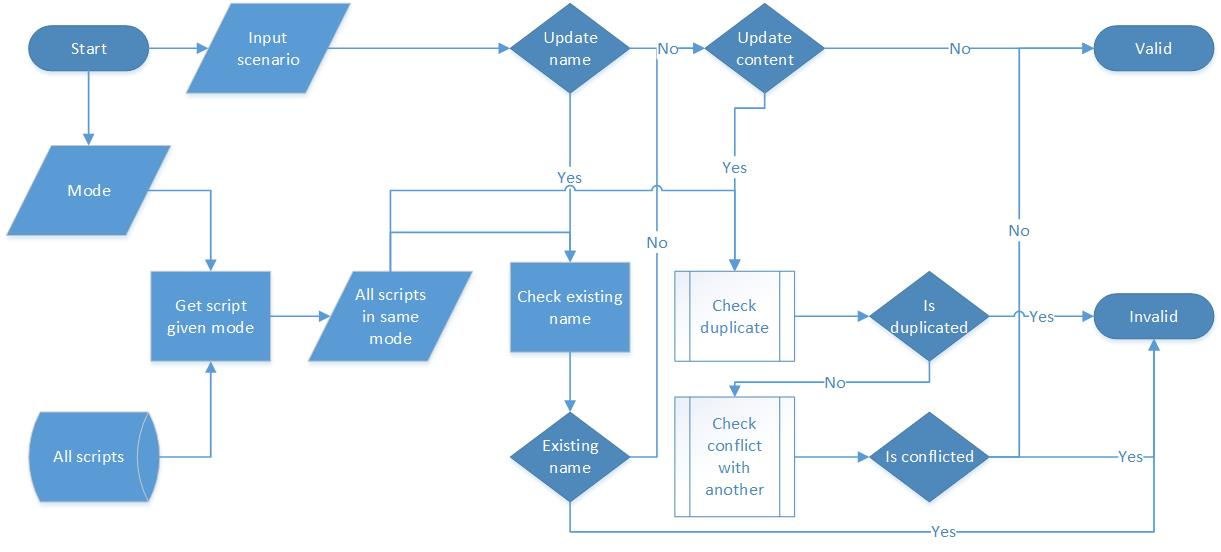
\includegraphics[width=15cm]{6-Flowchart-Scenario-Validator-Check-valid-scenario}
  \caption{Flowchart thể hiện cách kiểm tra kịch bản hợp lệ}\label{fig:6-Flowchart-Scenario-Validator-Check-valid-scenario}
\end{figure}

\noindent
Đầu vào thuật toán nhận một kịch bản cần kiểm tra tính hợp lệ (gọi là “input scenario”), còn đầu ra của thuật toán sẽ là giá trị luận lý đúng hoặc sai, tương ứng kịch bản hợp lệ hoặc không hợp lệ. Hình \ref{fig:6-Flowchart-Scenario-Validator-Check-valid-scenario} thể hiện thuật toán kiểm tra tính hợp lệ của kịch bản. Dựa trên thông tin về chế độ (mode) khi kịch bản được thêm vào hệ thống thì ta sẽ lấy tất cả kịch bản trong cùng chế độ ấy lên từ cơ sở dữ liệu. Mục đích của công việc này là kiểm tra xem tên của kịch bản mới (nếu có) có trùng với những kịch bản có sẵn hay không. Nếu trùng tên xảy ra thì kết luận rằng kịch bản đầu vào không hợp lệ. Kế tiếp, ta cần kiểm tra rằng nội dung kịch bản có bị trùng với kịch bản nào có sẵn chưa (xét trùng về mặt ngữ nghĩa chứ không chỉ là về mặt chuỗi lưu trữ kịch bản có giống nhau hoàn toàn hay không). Cuối cùng, thuật toán kiểm tra kịch bản mâu thuẫn sẽ được thực thi (chi tiết thuật toán được mô tả ở mục sau). Nếu kịch bản đầu vào không xảy ra mâu thuẫn với các kịch bản sẵn có thì kết quả trả về từ thuật toán là hợp lệ, trường hợp khác sẽ là không hợp lệ.

\subsubsection{Thuật toán kiểm tra kịch bản mâu thuẫn}

\begin{figure}[h]
  \centering
     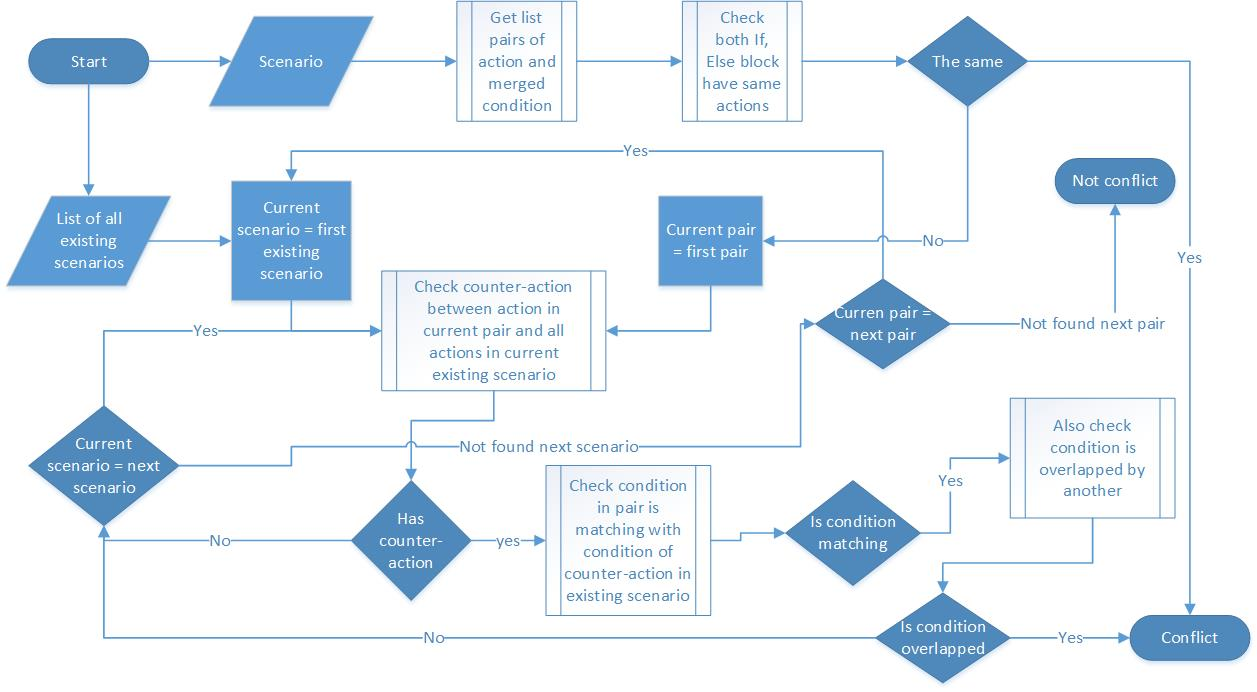
\includegraphics[width=15cm]{6-Flowchart-Scenario-Validator-How-to-check-conflict}
  \caption{Flowchart thể hiện cách kiểm tra kịch bản mâu thuẫn}\label{fig:6-Flowchart-Scenario-Validator-How-to-check-conflict}
\end{figure}

\noindent
Như đã đề cập về khái niệm kịch bản mâu thuẫn, trong thực tế nếu sự mâu thuẫn giữa các kịch bản tồn tại, hệ thống sẽ gặp nhiều rắc rối. Do đó, việc xử lý, ngăn chặn kịch bản mâu thuẫn là thiết yếu phải có của hệ thống. Hình \ref{fig:6-Flowchart-Scenario-Validator-How-to-check-conflict} mô tả tổng quan về thuật toán kiểm tra kịch bản mâu thuẫn. Đầu vào của thuật toán là kịch bản hệ thống muốn kiểm tra, cùng với danh sách kịch bản đã tồn tại trong cùng chế độ.\\

\noindent
Bước đầu, ta cần trích xuất ra từ kịch bản đầu vào những cặp <điều kiện gộp, hành động đơn giản> (<merged condition, simple action>) giúp cho việc so sánh. Nếu như kịch bản có tất cả 3 hành động đơn giản (simple action) thì ta sẽ có ít nhất 3 cặp <điều kiện gộp, hành động đơn giản> như trên. Một lưu ý nhỏ là <điều kiện gộp> có thể không tồn tại. Một điều kiện bên ngoài có thể gộp được với điều kiện lồng trong nó khi và chỉ khi 2 điều kiện đó cùng thuộc về 1 thiết bị nào đó, hoặc là điều kiện về thời gian. Lấy ví dụ:

	\begin{itemize}[topsep=1mm,itemsep=-0.5mm]
	\item Kịch bản 1: “Nếu nhiệt độ thu được từ cảm biến nhiệt gần cửa sổ lớn hơn 40 độ và bé hơn 50 độ thì bật đèn phòng”. Điều kiện gộp ở đây sẽ là nhiệt độ nằm trong khoảng 40 độ và 50 độ.
	\item Kịch bản 2: “Nếu thời gian từ 0h đến 6h thì tắt đèn phòng, đồng thời trong khoảng thời gian đó, nếu thời gian từ 4h đến 5h thì bật thêm đèn hành lang”. Điều kiện gộp ở đây cho hành động bật đèn hành lang sẽ là “từ 4h đến 5h”.
	\vspace{1mm}
	\end{itemize}

\noindent
Tiếp theo, thuật toán còn kiểm tra cả việc nếu như kịch bản có dạng “If/Then/Else” thì hành động ở khối “Then” và khối “Else” không được giống nhau (giống về mặt ngữ nghĩa). Nếu không, thuật toán sẽ xếp loại kịch bản này là mâu thuẫn. Sau các bước trên, ta sẽ phải lặp trên tất cả kịch bản hiện tại, với mỗi kịch bản, ta so sánh các hành động đơn giản trong kịch bản ấy với từng hành động trong cặp <điều kiện gộp, hành động đơn giản>. Nếu 2 điều kiện đó là trái ngược nhau về mặt ngữ nghĩa (ví dụ một hành động kêu bật đèn phòng và một hành động khác kêu tắt đèn phòng) thì ta xét tiếp về điều kiện gộp của chúng có “trùng nhau” hay không. Khái niệm xét “trùng” điều kiện đã được nêu rõ ở mục \textbf{\ref{scenario-conflict} Thế nào là kịch bản mâu thuẫn}. Nếu duyệt đến hết danh sách kịch bản hiện tại và không tìm thấy dấu hiệu kịch bản mâu thuẫn, thuật toán trả về kết quả kịch bản không mâu thuẫn. Trường hợp ngược lại thì sẽ trả về là kịch bản mâu thuẫn và lỗi sẽ được thông báo cho người dùng trên giao diện. 

\subsection{Module quản lý trạng thái các kịch bản (scenario runner)}

\begin{figure}[h]
  \centering
     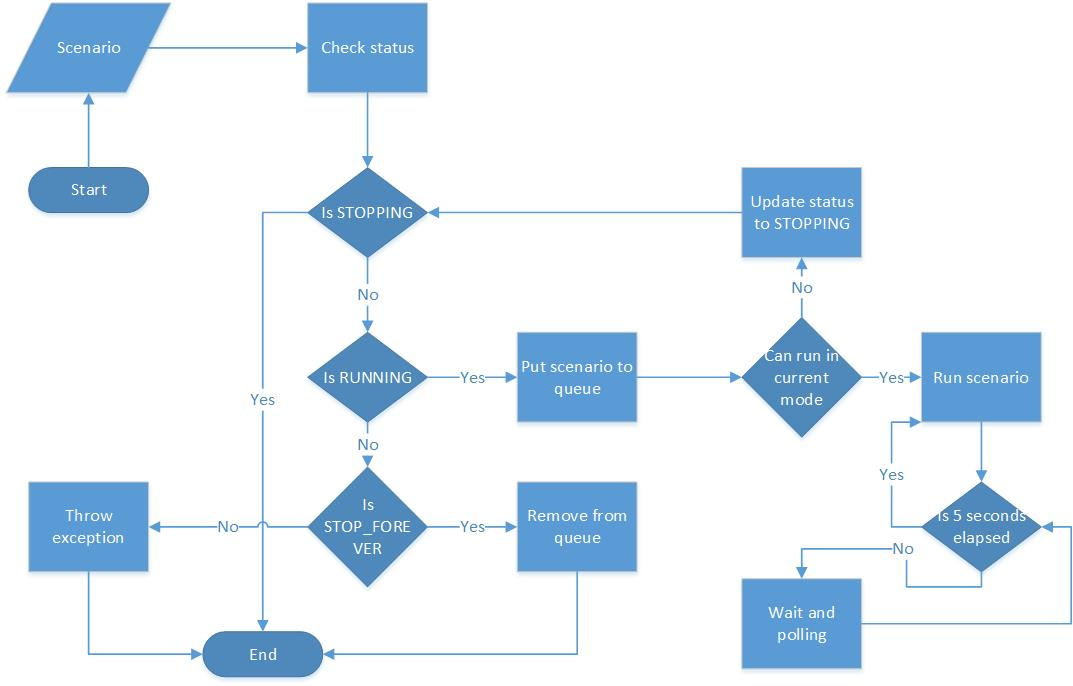
\includegraphics[width=15cm]{6-Flowchart-Scenario-Runner}
  \caption{Flowchart thể hiện cách quản lý trạng thái các kịch bản}\label{fig:6-Flowchart-Scenario-Runner}
\end{figure}

\noindent
Việc xây dựng kịch bản, cách thức tổ chức, cấu trúc dữ liệu kịch bản, … đều là tiền đề cho việc thực thi kịch bản đó. Nhóm đã phải đắn đó trong việc chọn cách thiết kế cấu trúc dữ liệu để việc quản lý, cũng như thực thi kịch bản dễ dàng và suôn sẻ hơn. Đáp ứng cho nhu cầu quản lý ấy, nhóm tạo ra module Scenario Runner. Đầu vào của module này sẽ là một kịch bản hệ thống với mong muốn là hệ thống sẽ thực thi, “chạy” kịch bản ấy. Hình \ref{fig:6-Flowchart-Scenario-Runner} mô tả thuật toán quản lý trạng thái các kịch bản trong hệ thống. Đầu vào thuật toán nhận kịch bản hệ thống với trạng thái xác định. Nếu trạng thái là dừng (STOP), module lập tức cập nhật ngay trạng thái đó vào kịch bản tương ứng trong hàng chờ hệ thống và làm nó dừng thật sự. Nếu trạng thái là chạy (RUNNING), ta cần kiểm tra thêm 1 điều kiện đó là kịch bản này có thể chạy ở chế độ hiện tại hay không. Nếu có thì cứ sau khoảng thời gian mặc định, tầm 5 giây, kịch bản được kích hoạt hàm chạy một lần. Và ngược lại, nếu kịch bản không thuộc về chế độ hiện tại của nhà này, trạng thái kịch bản sẽ cập nhật thành dừng và nằm trong hàng chờ hệ thống. Trường hợp mà người dùng mong muốn xóa đi kịch bản, trạng thái của nó sẽ trở thành dừng vĩnh viễn và được loại bỏ khỏi hàng chờ.\\

\noindent
Module Scenario Runner quản lý mỗi kịch bản bởi 1 thread khác nhau, nói cách khác là chịu trách nhiệm xử lý multi-thread. Mỗi kịch bản cứ sau khoảng 5 giây sẽ được chạy lại một lần, nhằm đảm bảo mọi cập nhật mới nhất với kịch bản ấy có hiệu lực gàn như lập tức. Kịch bản thì có chứa thông tin về trạng thái: chạy, dừng, dừng vĩnh viễn. Nhiệm vụ module này cũng là kiểm soát trạng thái các kịch bản ấy.\\

\noindent
Sau khi một kịch bản mới được thêm vào hệ thống, trạng thái của nó sẽ là chạy (RUNNING). Khi kịch bản ấy được cập nhật, trạng thái của nó cũng được cập nhật lại. Nếu như người dùng muốn cho phép (enable) hoặc vô hiệu hóa (disable) ngôi nhà, hay thiết bị có liên quan kịch bản ấy thì thao tác đó cũng làm ảnh hưởng đến trạng thái của kịch bản. Ví dụ người dùng cho phép dùng (enable) thiết bị ấy thì các kịch bản liện quan thiết bị đó sẽ mang trạng thái đang chạy (RUNNING). Khi người dùng vô hiệu hóa thiết bị, các kịch bản liên quan sẽ chuyển sang trạng thái dừng (STOP). Tương tự với việc cho phép sử dụng nhà hay vô hiệu hóa nhà thì kịch bản thuộc nhà ấy cũng có trạng thái chạy hay dừng tương ứng.\\

\noindent
Tuy nhiên, vấn đề quản lý multi-thread hiệu quả khi số lượng kịch bản tăng lên cũng là một khó khăn mà nhóm đang đối mặt và sẽ được đề cập tới trong mục thảo luận.

\subsection{Module hỗ trợ xác thực và phân quyền (authorization and authentication)}

Xác thực (authentication) và phân quyền (authorization) là một vấn đề không thể thiếu trong nhà thông minh, làm thế nào để có thể xây dựng một ngôi nhà mang tính bảo mật cao, không cho phép người ngoài có thể xâm nhập vào ngôi nhà của mình là một đề tài khó.\\

\noindent
Trong hệ thống của chúng tôi, việc bảo mật (security) cho ngôi nhà được chia làm hai bước:

\begin{itemize}[topsep=1mm,itemsep=-0.5mm]
	\item Xác thực: Người dùng cần nhập đúng tên đăng nhập và mật khẩu đã đăng ký trước đó để có thể đăng nhập vào hệ thống.
	\item Phân quyền: Sau khi đã xác thực thành công, tại mỗi yêu cầu truy xuất tài nguyên mà người dùng gửi lên, hệ thống sẽ kiểm tra xem người dùng có quyền để truy xuất tài nguyên đó hay không, tức kiểm tra người dùng có đúng là chủ nhân thật sự của ngôi nhà đó hay không. Hệ thống chúng tôi thiết kế cho phép một người có thể sở hữu nhiều căn nhà khác nhau.
	\vspace{1mm}
	\end{itemize}
	
Do client tương tác với server chủ yếu bằng các web service mà server cung cấp, nên phương pháp xác thực thường được sử dụng phổ biến là sử dụng mã xác thực (token). Sau khi người dùng đã đăng nhập thành công, tức nhập đúng tên đăng nhập và mật khẩu, hệ thống sẽ gửi một mã xác thực đến người dùng. Từ đó về sau, khi muốn gửi một yêu cầu đến server, client cần gửi lại đúng mã xác thực mà server đã gửi trước đó, nếu sai, hệ thống sẽ báo lỗi không có quyền truy cập (unauthorized). Mô hình xác thực giữa client và server được mô tả tại hình \ref{fig:6-authentication}.\\

\begin{figure}[h]
  \centering
     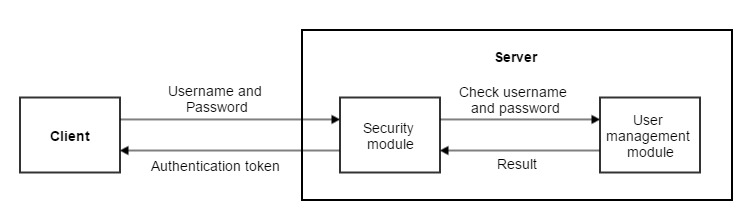
\includegraphics[width=15cm]{6-authentication}
  \caption{Mô hình xác thực người sử dụng}\label{fig:6-authentication}
\end{figure}

\noindent
Sau khi người dùng đã gửi đúng mã xác thực, server sẽ tiến hành kiểm tra xem người dùng có quyền đối với căn nhà hay không. Từ tên đăng nhập của người dùng mà client gửi liên, server sẽ tìm ra danh sách tất cả ngôi nhà thuộc sở hữu của người sử dụng. Nếu ngôi nhà mà người dùng đang muốn điều khiển nằm trong danh sách những ngôi nhà thuộc quyền sở hữu của người sử dụng, hệ thống sẽ cho phép người dùng truy xuất tài nguyên của căn nhà, ngược lại, hệ thống sẽ báo lỗi không có quyền truy cập. Hình \ref{fig:6-authorization} mô tả chi tiết bước phân quyền của hệ thống nhà thông minh.

\begin{figure}[h]
  \centering
     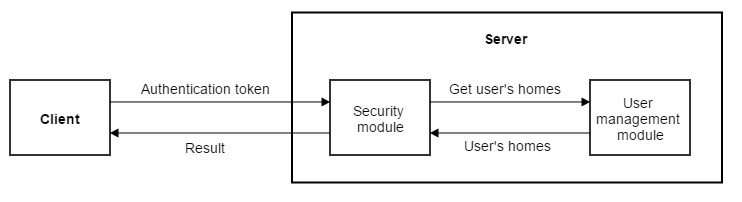
\includegraphics[width=15cm]{6-authorization}
  \caption{Mô hình phân quyền người sử dụng}\label{fig:6-authorization}
\end{figure}

\noindent
Bên cạnh đó, phương thức giao tiếp giữa client và server là https nên dữ liệu trao đổi qua lại trên đường truyền đều được mã hóa, tránh trường hợp hacker đánh cắp tài khoản người dùng hoặc thực hiện hành vi xấu.

\subsection{Đánh giá hiện thực back-end}
\noindent
Qua chi tiết phần hiện thực back-end, ta có được một cái nhìn chi tiết hơn, sâu hơn về phần thiết kế hệ thống back-end. Back-end đóng vai trò là trung tâm, là “bộ não” của toàn hệ thống, lưu trữ các dữ liệu quan trọng của người dùng,\dots\hspace{0mm} cho nên khâu thiết kế, xây dựng và hiện thực cần tiến hành kĩ lưỡng, cân nhắc đến nhiều vấn đề liên quan. Hệ thống back-end được xây dựng theo hướng module hóa, mỗi module đảm nhận nhiệm vụ chuyên biệt. Trong đó, quan trọng nhất chính là các module chuyển đổi sang kịch bản hệ thống, module kiểm tra tính hợp lệ và module quản lý, khởi chạy các kịch bản. Tuy rằng hệ thống chưa thực sự hoàn thiện, việc quản lý tài nguyên, quản lý kịch bản chưa được tối ưu, dạng kịch bản chưa phong phú, đa dạng,\dots\hspace{0mm} nhưng với bước khởi điểm này cùng những định hướng mở rộng trong tương lai thì hệ thống sẽ có tính khả thi và thực tiễn cao hơn.

\section{Xây dựng module điều khiển thiết bị}\label{device-controller-implementation}
\subsection{Lắp đặt thiết bị}
Để Raspberry Pi có thể điều khiển được các thiết bị thông qua các chân GPIO, đầu tiên, chúng ta phải lắp đặt đúng cách thiết bị đó vào Raspberry Pi. Nhằm mục đích đảm bảo an toàn và thuận tiện trong việc tiến hành thí nghiệm, chúng tôi ưu tiên sử dụng những thiết bị điện yêu cầu hiệu điện thế thấp (từ 5V trở xuống).

\begin{figure}[h]
  \centering
     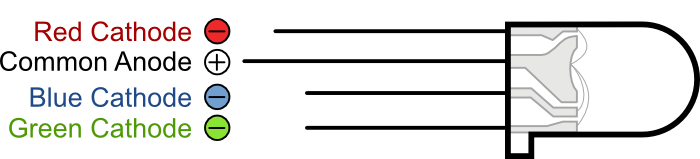
\includegraphics[width=10cm]{6-rgb-led}
  \caption{Thông tin các chân của đèn led}\label{fig:6-rgb-led}
\end{figure}

\noindent
\textbf{Lắp đặt đèn:} Đèn được sử dụng trong thí nghiệm là loại đèn led bốn chân tích cực mức cao. Một chân của đèn led sẽ luôn luôn được nối vào cổng Ground của Raspberry Pi, một chân còn lại (chân red, green hoặc blue) sẽ được nối vào một GPIO. Khi GPIO ở trạng thái High, tức mức điện áp đưa vào là 3.3V, đèn led sẽ sáng, ngược lại, đèn sẽ tắt. Hình \ref{fig:6-rgb-led} trình bày thông tin các chân của đèn led. Ngoài led ba màu, nhóm còn sử dụng thêm loại led chỉ có hai chân được sử dụng rộng rãi, cách lắp đặt tương tự như đèn led bốn chân.\\

\noindent
\textbf{Lắp đặt còi:} Còi là một thiết bị không thể thiếu trong các căn nhà thông minh, mục đích chủ yếu là để cảnh báo chủ nhà đang có nguy hiểm xảy ra. Loại còi được nhóm sử dụng trong mô hình nhà thông minh gồm có ba chân: VCC, GND và Signal. Hình \ref{fig:6-buzzer} mô tả vị trí các chân nằm trên module còi. Hai chân VCC và GND sẽ lần lượt được gắn vào hai cổng luôn luôn có hiệu điện thế lần lượt là 3.3V và 0V, chân Signal sẽ được gắn vào một cổng GPIO có nhiện vụ điều khiển. Loại còi mà nhóm sử dụng thuộc loại tích cực mức thấp nên còi sẽ bắt đầu hú khi trạng thái của GPIO điều khiển là Low.

\begin{figure}[h]
  \centering
     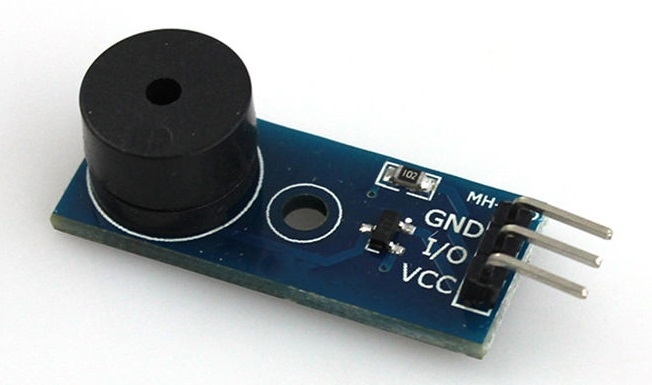
\includegraphics[width=5cm]{6-buzzer}
  \caption{Module còi gồm 3 chân: VCC, GND và Signal (nằm giữa)}\label{fig:6-buzzer}
\end{figure}

\noindent
\textbf{Lắp đặt cảm biến khí gas:} Với các đặc tính như giá thành rẻ, độ nhạy cao và phạm vi phát hiện rộng, cảm biến khí gas MQ-2 được nhóm sử dụng để phát hiện sự xuất hiện của các khí dễ cháy như gas, cồn và khói. Cảm biến gồm có bốn chân: VCC, GND, DOUT và AOUT, hình \ref{fig:6-gas-sensor} mô tả cấu trúc bên ngoài của một cảm biến khí gas. Các chân VCC và GND lần lượt sẽ được nối vào các cổng có hiệu điện thế là 3.3V và 0V. Khi phát hiện khí gas, cổng AOUT sẽ xuất ra tính hiện tương tự (analog) còn cổng DOUT sẽ xuất ra tín hiện số (digital).

\begin{figure}[h]
  \centering
     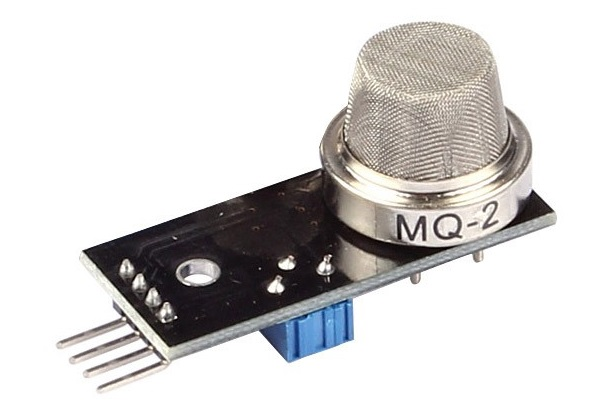
\includegraphics[width=5cm]{6-gas-sensor}
  \caption{Module cảm biến khí gas MQ-2}\label{fig:6-gas-sensor}
\end{figure}

\noindent
Do đặc tính các chân GPIO của Raspberry Pi chỉ nhận được tín hiệu số, nên chúng tôi chỉ sử dụng chân DOUT của cảm biến để phát hiện khí gas. Chân DOUT sẽ được đấu nối với một cổng GPIO của Raspberry PI. Bình thường, chân DOUT của cảm biến sẽ ở trạng thái High, tức có mức điện áp là 3.3V, khi phát hiện khí gas, chân DOUT sẽ ngay lập tức chuyển từ trạng thái High thành Low (0V), và trạng thái này kéo dài cho đến khi cảm biến không còn phát hiện khí gas trong không khí. Độ nhạy của cảm biến sẽ được điều chỉnh bằng tay thông qua bộ điều chỉnh màu xanh đặc bên dưới cảm biến \cite{gas-sensor}.\\

\noindent
\textbf{Lắp đặt cảm biến ánh sáng:} Module cảm biến ánh sáng sử dụng quang trở được lựa chọn sử dụng để phát hiện thời gian hiện tại là ban ngày hay ban đêm. Khi cường độ ánh sáng tăng, điện trở của quang trở sẽ giảm và ngược lại, khi cường độ ánh sáng giảm, điện trở sẽ tăng. Giống module cảm biến khí gas MQ-2, module cảm biến ánh sáng sử dụng quang trở cũng có ba chân: VCC, GND và Signal. VCC và GND cũng sẽ được nối vào hai cổng có hiệu điện thế lần lượt là 3.3V và 0V, chân Signal được nối vào một công GPIO của Raspberry Pi.\\

\noindent
Khi cường độ ánh sáng thấp hơn giá trị ngưỡng, cổng Signal sẽ ở trạng thái High, tức có hiệu điện thế là 3.3V. Khi cường độ ánh sáng vượt quá giá trị ngưỡng, cổng Signal sẽ ở trạng thái Low, tức có hiệu điện thế là 0V. Giá trị ngưỡng được điều chỉnh bằng  tay sử dụng nút vặn màu xanh nằm phía dưới cảm biến. Hình \ref{fig:6-light-sensor} mô tả một con Raspberry Pi đã được kết nối với module cảm biến ánh sáng quang trở \cite{light-sensor}\cite{light-sensor-2}.

\begin{figure}[h]
  \centering
     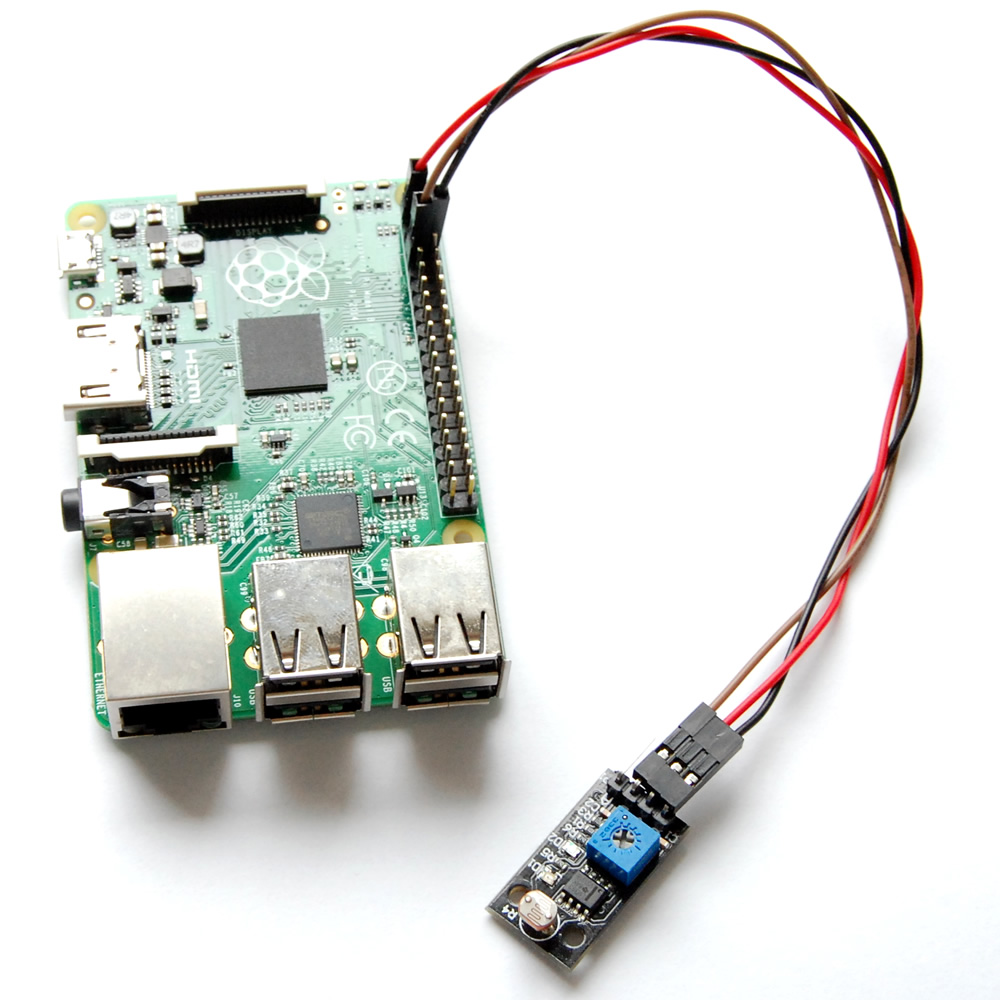
\includegraphics[width=6cm]{6-light-sensor}
  \caption{Module cảm biến ánh sáng quang trở được gán vào Raspberry Pi}\label{fig:6-light-sensor}
\end{figure}

\noindent
\textbf{Lắp đặt cảm biến chuyển động:} Chức năng chống trộm cũng là một chức năng không thể thiếu của một ngôi nhà thông minh. Nhóm sử dụng module cảm biến chuyển động PIR (Passive InfraRed) để nhận biết có người hay có trộm vừa đi ngang qua. Nguyên lý hoạt động của cảm biến là dựa vào bức xạ nhiệt mà con người phát ra. Mỗi người trong chúng ta đều có thân nhiệt lúc bình thường khoảng 37 độ C và đều phát ra các bức xạ nhiệt. Khi một người đi qua, các tia bức xạ nhiệt phát ra từ người đó sẽ kích hoạt cảm biến. Hình \ref{fig:6-pir-sensor} mô tả cấu trúc bên ngoài cảm biến chuyển động PIR \cite{pir-sensor}.

\begin{figure}[h]
  \centering
     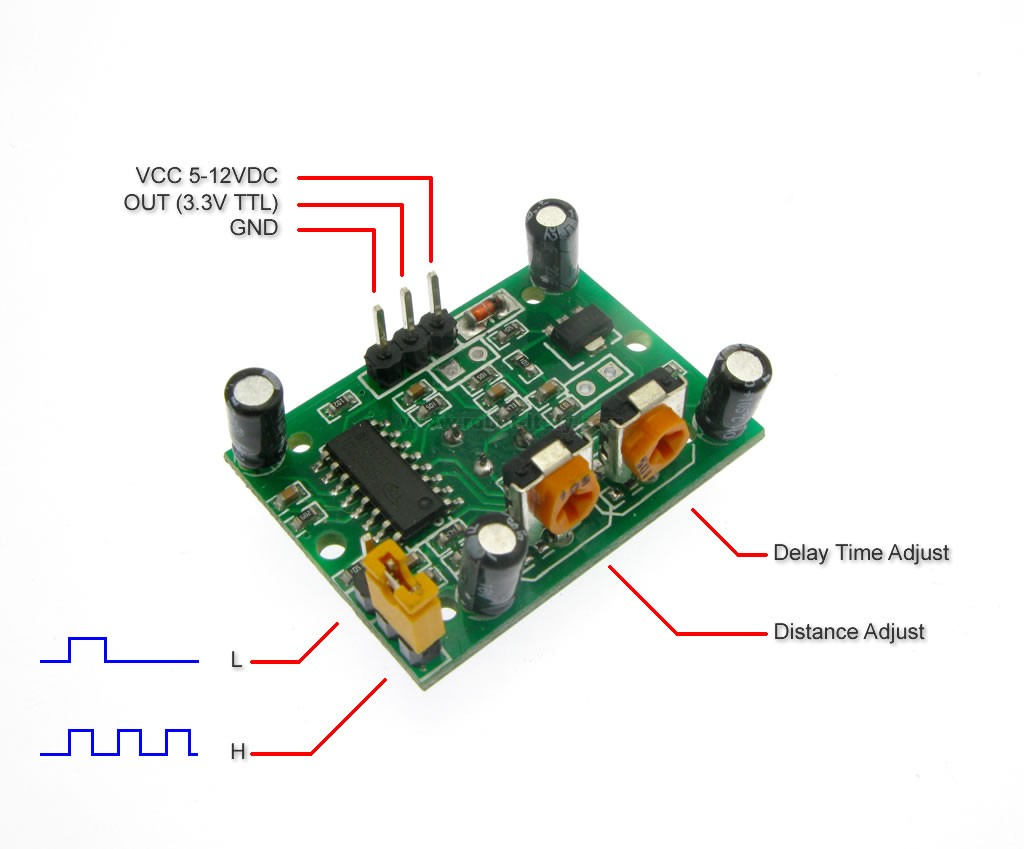
\includegraphics[width=7cm]{6-pir-sensor}
  \caption{Cảm biến chuyển động PIR}\label{fig:6-pir-sensor}
\end{figure}

\noindent
Cảm biến có ba chân: VCC, GND và OUT. Cổng VCC và GND sẽ lần lượt nối vào các cổng có hiệu điện thế lần lượt là 5V và 0V trên Raspberry Pi. Cổng OUT sẽ được nối vào một chân GPIO để ứng dụng trên Raspberry Pi có thể lấy dữ liệu từ cảm biến. Bình thường, khi không có người đi ngang qua, cổng OUT sẽ có trạng thái là Low, khi phát hiện người, trạng thái của cổng OUT là High. Khoảng cách phát hiện người và độ trễ của cảm biến có thể được điều chỉnh bằng tay qua hai bộ điều chỉnh màu cam đặt ở một cạnh của cảm biến.\\

\noindent
\textbf{Lắp đặt cảm biến nhiệt độ:} Nhóm sử dụng cảm biến nhiệt độ DS18B20 để lấy giữ liệu về nhiệt độ trong hệ thống nhà thông minh. Cách lắp đặt cảm biến nhiệt độ này có chút phức tạp hơn so với các cảm biến khác. Cảm biến cũng gồm có ba chân: VCC, GND và OUT. Giống như các cảm biến khác, cổng VCC và GND cũng được lần lượt gắn vào các cổng có hiệu điện thế lần lượt là 3.3V và 0V. Tuy nhiên, khác với các cảm biến khác, cổng OUT của cảm biến nhiệt độ DS18B20 phải được gắn vào GPIO số 4 nằm ở vị trí số 7 trên Raspberry Pi. Bên cạnh đó, phải có một điện trở 4.7 ôm nối giữa VCC và OUT. Đầu màu vàng của cảm biến điện trở sẽ được nối vào dây VCC của cảm biến nhiệt độ. Hình \ref{fig:6-temp-sensor} mô tả cách lắp ghép cảm biến nhiệt độ DS18B20 vào Raspberry Pi.

\begin{figure}[h]
  \centering
     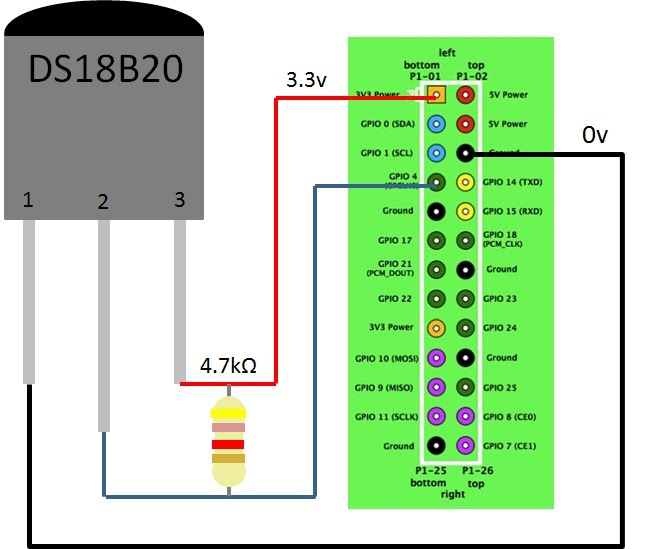
\includegraphics[scale=0.3]{6-temp-sensor}
  \caption{Cách mắc dây cho cảm biến nhiệt độ DS18B20 [11]}\label{fig:6-temp-sensor}
\end{figure}

\noindent
Do cảm biến DS18B20 sử dụng cơ chế truyền tín hiệu 1-Wire nên cho phép người sử dụng có thể kết nhiều cảm biến vào cùng một chân trên Raspberry Pi. Cách kết nối cũng vô cùng đơn giản, chỉ cần kết nối tất cả cổng OUT của tất cả cảm biến vào cùng chân GPIO số 4 của Raspberry Pi \cite{temp-sensor}.

%------------------------------Hiện thực module----------------------------%
\subsection{Hiện thực module điều khiển thiết bị}

Module điều khiển thiết bị được chia làm nhiều bộ điều khiển nhỏ cho các loại thiết bị và được quản lý bởi bộ điều chung. Tất cả các yêu cầu từ server sẽ được bộ điều khiển chung xử lý và đẩy vào các bộ điều khiển thích hợp. Bên cạnh đó, module điều khiển thiết bị còn có thêm bộ cung cấp GPIO với nhiệm vụ khởi tạo đúng loại cổng mà một bộ điều khiển cần. Hình \ref{fig:6-module-dieu-khien-class-diagram} thể hiện sơ đồ lớp (class diagram) của module.

\begin{figure}[h]
  \centering
     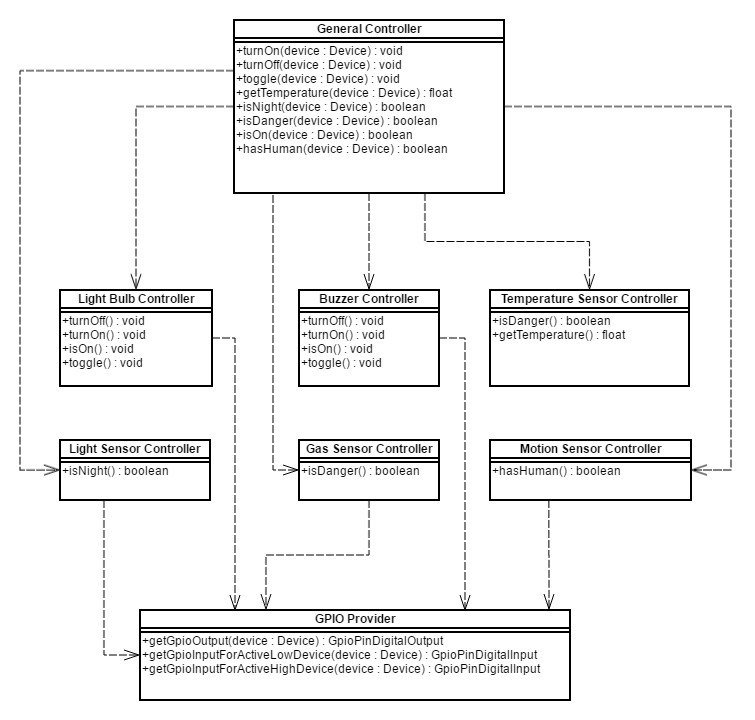
\includegraphics[width=15.5cm]{6-module-dieu-khien-class-diagram}
  \caption{Sơ đồ lớp (class diagram) của module điều khiển thiết bị}\label{fig:6-module-dieu-khien-class-diagram}
\end{figure}

\noindent
\textbf{Bộ điều khiển chung (GPIO Controller):} Như đã trình bày, bộ điều khiển chung sẽ nhận tất cả yêu cầu từ server. Bộ điều khiển chung cung cấp tất cả các phương thức mà server cần để lấy dữ liệu từ cảm biến cũng như điều khiển các thiết bị điện. Để sử dụng một hàm, server cần truyền vào một thực thể device. Thực thể device sẽ cung cấp tất cả các thông tin mà bộ điều khiển chung cần để thực hiện đúng hành động vào đúng thiết bị mà server cần như loại thiết bị, số thứ tự cổng GPIO,\dots\hspace{0mm} Bộ điều khiển chung sẽ dựa vào thông tin loại thiết bị và quyết định nên sử dụng bộ điều khiển thiết bị nào phù hợp. Ví dụ, server gửi yêu cầu tắt một thiết bị, trong yêu cầu của server sẽ chứa thông tin loại thiết bị mà server muốn tắt (đèn, còi,\dots) kèm theo số thứ tự của cổng GPIO đang điều khiển thiết bị đó. Nếu loại thiết bị là đèn, bộ điều khiển chung sử dụng bộ điều khiển đèn (Light bulb controller) để thực hiện phương thức tắt.\\

\noindent
\textbf{Bộ cung cấp GPIO (GPIO Provider):} Trong thư viện Pi4J, để sử dụng một cổng GPIO, bước đầu tiên là khai báo cổng cần sử dụng. Bộ cung cấp GPIO có nhiệm vụ hỗ trợ các bộ điều khiển thiết bị thực hiện thao tác khai báo một cổng GPIO. Tùy thuộc vào mục đích mà một cổng GPIO có thể được khai báo là cổng nhập (input pin) hay cổng xuất (output pin). Cổng nhập (input pin) được các bộ điều khiển cảm biến sử dụng để lấy dữ liệu từ các cổng GPIO. Cổng xuất (output pin) được bộ điều khiển đèn và còi sử dụng để điều khiển việc bật hoặc tắt. Cú pháp khai báo một cổng GPIO được trình bày ở đoạn code sau:

\begin{lstlisting}[language=Java, label={lst:declare-gpio}]
	final GpioPinDigitalOutput outputPin = gpio.provisionDigitalOutputPin(
					RaspiPin.GPIO_01, "MyLED", PinState.HIGH);
\end{lstlisting}

\begin{figure}[h]
  \centering
     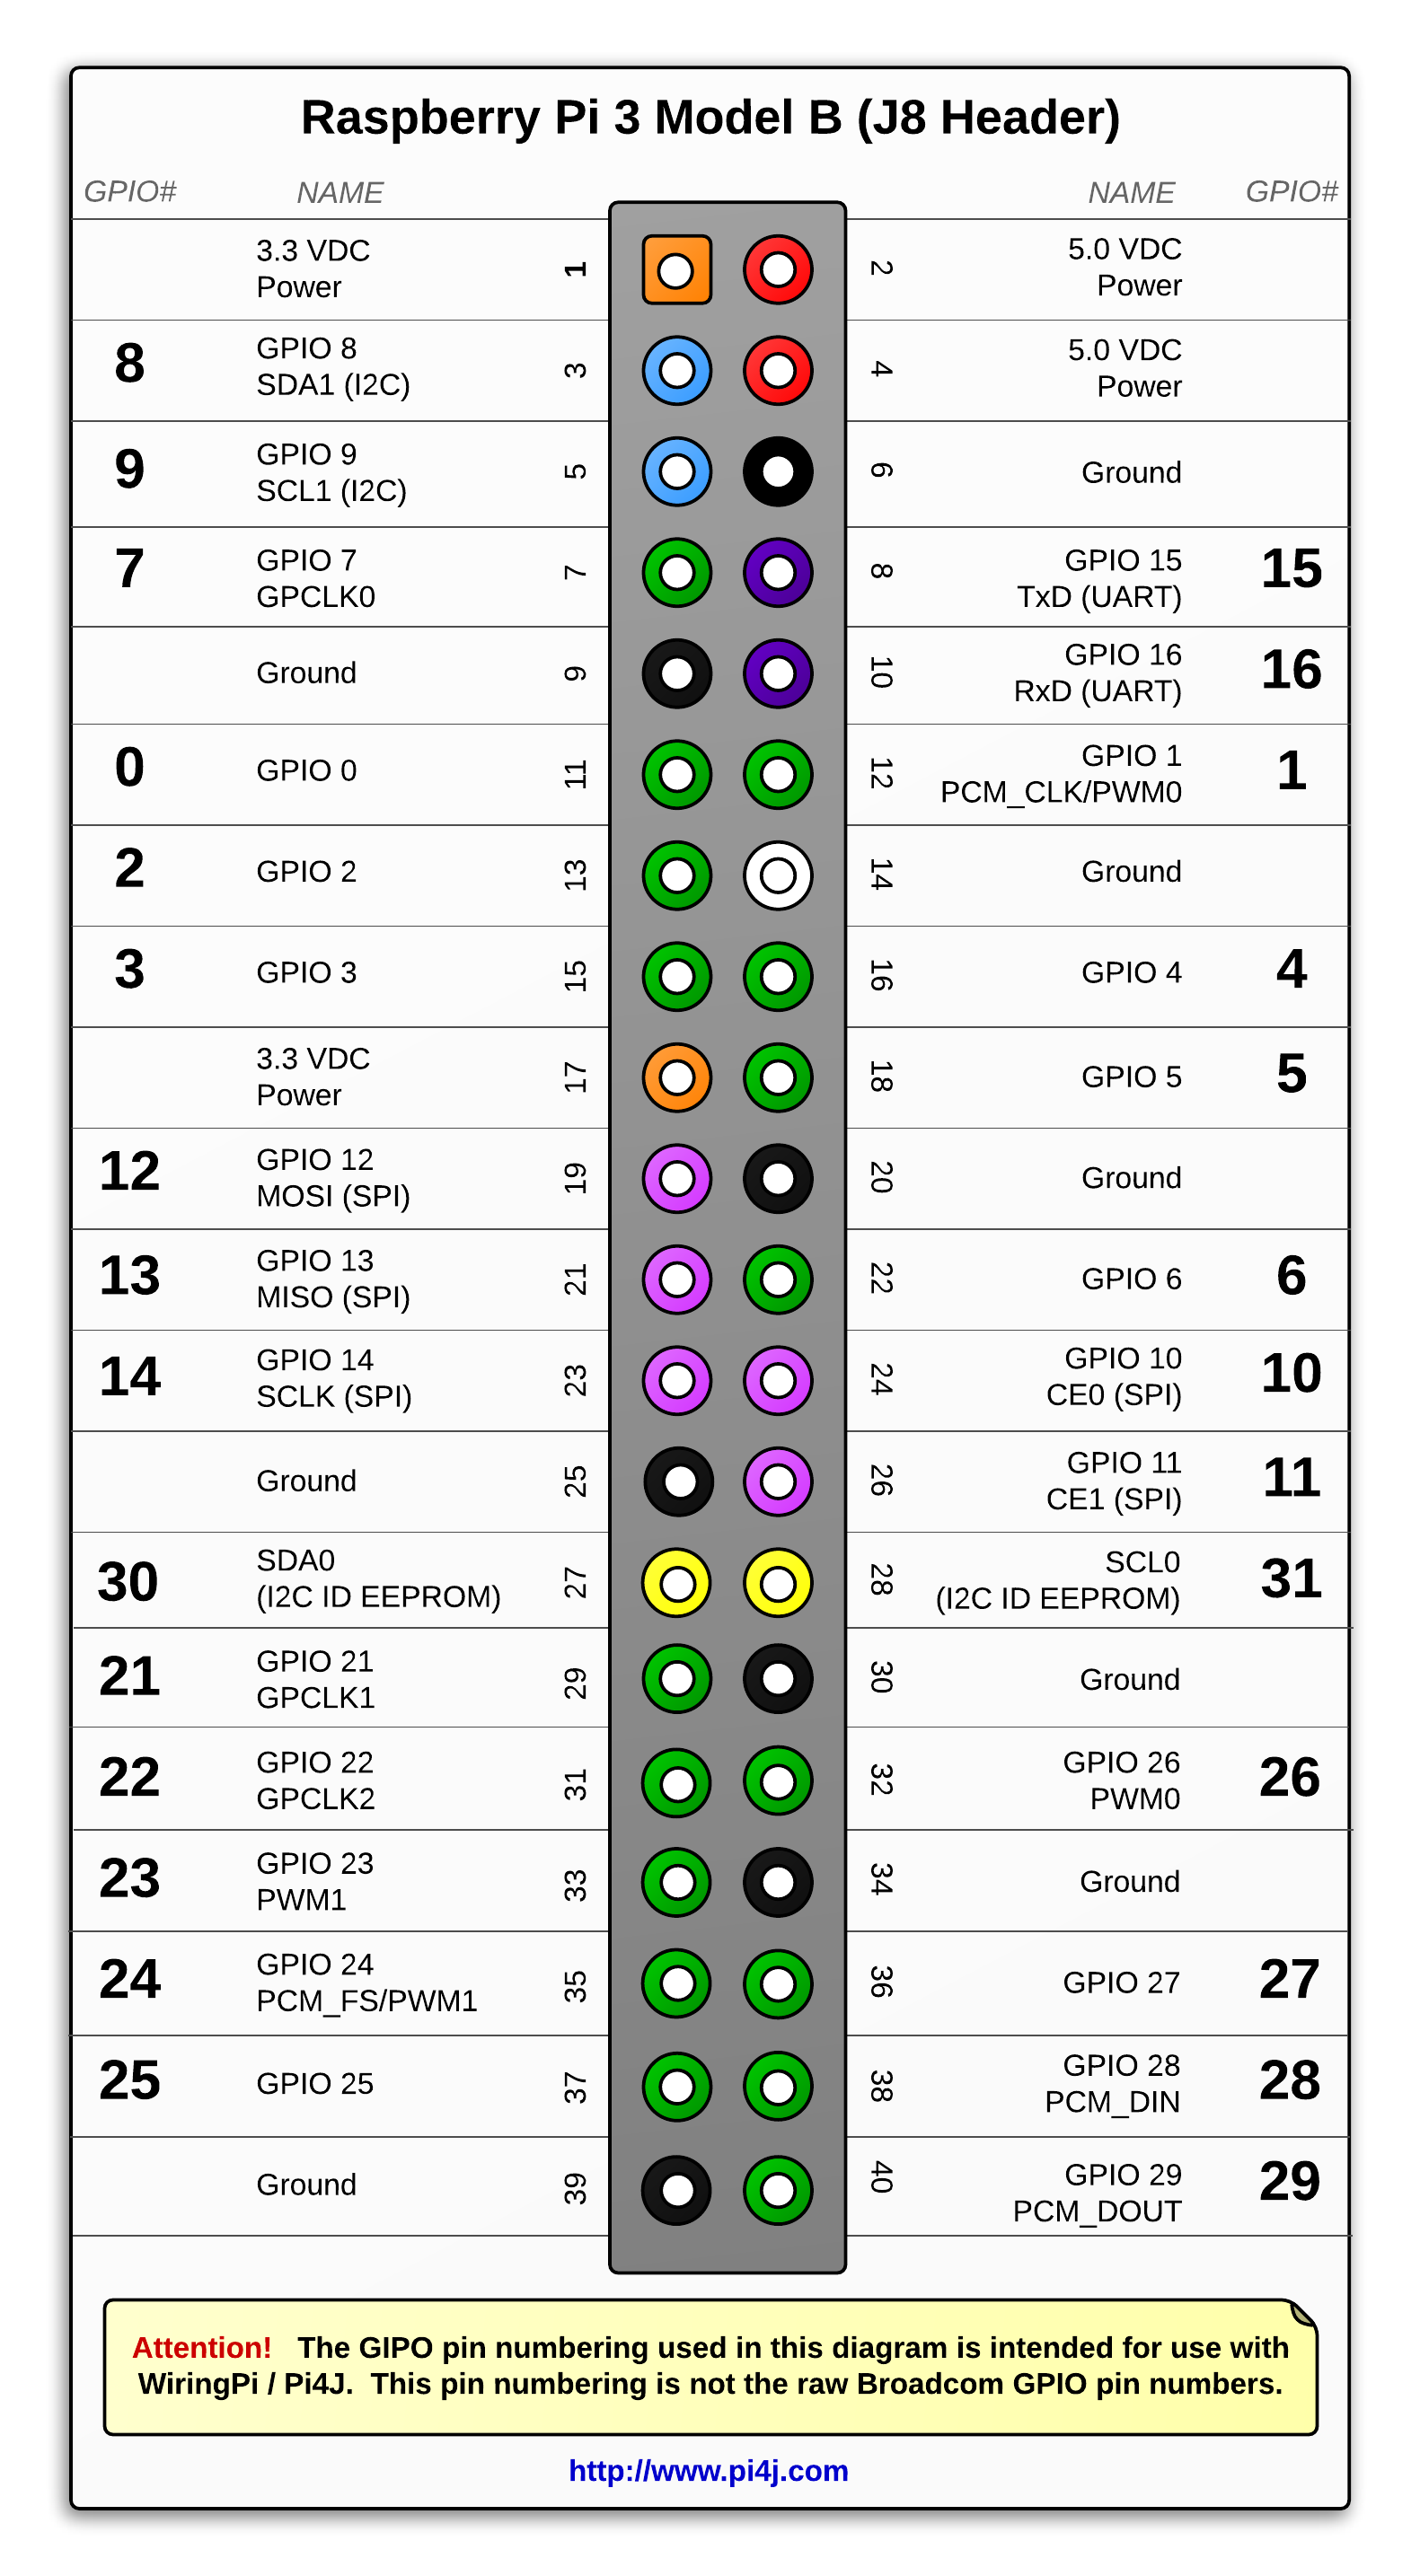
\includegraphics[width=7cm]{4-pi4j-danh-so}
  \caption{Quy tắc đánh số của Pi4J cho Raspberry Pi 3 Model B}\label{fig:4-pi4j-danh-so}
\end{figure}

\noindent
Để tránh những sự thay đổi về phần cứng sẽ ảnh hưởng đến phần mềm sử dụng các chân GPIO của Raspberry Pi, Pi4J sử dụng bộ quy tắc đánh số riêng cho những cổng GPIO. Vì thế, bộ cung cấp GPIO còn giữ vai trò chuyển đổi số thứ tự một cổng GPIO trên Raspberry Pi về số thứ tự hợp lệ trên Pi4J. Hình \ref{fig:4-pi4j-danh-so} mô tả cách đánh số của thư viện Pi4J trên Raspberry Pi 3 Model B. Ví dụ, cổng GPIO ở vị trí 11 trên Raspberry Pi khi chuyển đổi sang cách đánh số của thư viện Pi4J sẽ có số thứ tự là GPIO 0 \cite{pi4j-numbering}.\\

\noindent
\textbf{Bộ điều khiển đèn và bộ điều khiển còi:} Hai bộ điều khiển này được sử dụng bởi bộ điều khiển chung khi server có các yêu cầu liên quan đến đèn và còi. Sau khi nhận yêu cầu từ server, bộ điều khiển chung sẽ truyền thông tin về thiết bị đến đúng bộ điều khiển thích hợp. Khi nhận thông tin về thiết bị bao gồm số thứ tự cổng GPIO, bộ điều khiển đèn hoặc còi sẽ sử dụng bộ cung cấp GPIO để khởi tạo đúng loại cổng, input pin hay output pin.\\

\noindent
Như đã trình bày, mỗi cổng GPIO sẽ có hai trạng thái là Low hoặc High. Bộ điều khiển đèn và còi sẽ điều khiển các thiết bị bằng cách thay đổi trạng thái của chân GPIO đang điều khiển thiết bị đó. Tùy loại thiết bị mà trạng thái High hoặc Low sẽ tương ứng với việc bật hay tắt và ngược lại. Ví dụ, nếu loại đèn được sử dụng là tích cực mức thấp, khi chân GPIO ở trạng thái Low thì đèn sẽ sáng và ngược lại. Loại đèn và còi mà nhóm đang sử dụng để thuộc loại tích cực mức thấp. Cú pháp thay đổi trạng thái một cổng GPIO khi sử dụng thư viện Pi4J thể hiện như sau:

\begin{lstlisting}[language=Java, label={lst:change-state-gpio}]
	outputPin.setState(PinState.LOW);
	outputPin.setState(PinState.HIGH);
\end{lstlisting}

\noindent
\textbf{Các bộ điều khiển cảm biến:} Tương tự như bộ điều khiển đèn và còi, các bộ điều khiển cảm biến cũng được sử dụng bởi bộ điều khiển chung khi server gửi một yêu cầu lấy dữ liệu từ các cảm biến đến bộ điều khiển chung. Tùy loại cảm biến mà cách lấy dữ liệu sẽ khác nhau, tuy nhiên, giống như đèn và còi, mỗi cảm biến sẽ được điều khiển bởi một GPIO nhất định.\\

\noindent
Đối với bộ điều khiển cảm biến khí gas, do loại cảm biến khí gas mà nhóm sử dụng thuộc loại tích cực mức thấp, tức bình thường, chân DOUT của cảm biến sẽ ở trạng thái High, khi phát hiện khí gas, lập tức chân DOUT sẽ chuyển sang trạng thái Low. Vì vậy, sau khi nhận thông tin về số thứ tự GPIO từ bộ điều khiển chung, bộ điều khiển khí gas cần nhờ sự hỗ trợ của bộ cung cấp GPIO để khai báo một cổng nhập phù hợp với loại cảm biến tích cực mức thấp. Sau khi đã khai báo xong, bộ điều khiển khí gas có thể lấy thông tin từ cảm biến bằng cách kiểm trang xem GPIO điều khiển cảm biến đang ở trạng thái High hay Low, vì GPIO điều khiển cảm biến sẽ được nối vào chân DOUT của cảm biến khí gas. Cú pháp kiểm tra khi sử dụng thư viện Pi4J cũng khá đơn giản, được thể hiện ở đoạn code sau:

\begin{lstlisting}[language=Java, label={lst:check-state-active-low}]
	activeLowPin.isLow();
\end{lstlisting}

\noindent
Khác với bộ điều khiển cảm biến khí gas, loại cảm biến ánh sáng và cảm biến chuyển động mà nhóm đang sử dụng thuộc loại tích cực mức cao, tức khi trời tối hoặc khi phát hiện có người chuyển động, cổng Signal của cảm biến ánh sáng và cổng OUT của cảm biến chuyển động sẽ ở trạng thái High. Vì vậy, cách khai báo cổng nhập cho hai bộ điều khiển này khác với bộ điều khiển cảm biến khí gas, cần sử dụng phương thức khai báo cổng nhập tích cực mức cao do bộ cung cấp GPIO hỗ trợ. Sau khi đã hoàn thành việc khai báo, công việc lấy dữ liệu từ cảm biến sẽ vô cùng đơn giản, chỉ cần kiểm tra xem cổng GPIO đang điều khiển cảm biến áng sáng hoặc cảm biến chuyển động có ở trạng thái High không, nếu có tức trời đang tối hoặc có người đang đi ngang qua. Cú pháp kiểm tra được thực hiện bởi đoạn code sau với sự hỗ trợ của thư viện Pi4J:

\begin{lstlisting}[language=Java, label={lst:check-state-active-high}]
	activeHighPin.isHigh();
\end{lstlisting}

\noindent
Trong tất cả các thiết bị cảm biến mà nhóm hiện có, cảm biến nhiệt độ là một trường hợp đặc biệt. Do cảm biến nhiệt độ mà nhóm sử dụng là DS18B20, sử dụng cơ chế truyền tín hiệu 1\-wire, có thể kết nối nhiều cảm biến vào chân GPIO số 4 của Raspberry Pi nên cách lấy dữ liệu sẽ khác với các cảm biến khác. Thông tin về nhiệt độ sẽ được để vào một tệp có tên là w1\_slave. Mỗi cảm biến nhiệt độ DS18B20 sẽ có một thư mục riêng chứ tệp w1\_slave, vì vậy, chúng ta cần vào đúng thư mục của cảm biến phù hợp. Cấu trúc thư mục của mỗi cảm biến chứ thông tin nhiệt độ là:
\begin{verbatim}
/sys/bus/w1/devices/<temperature-sensor-id>/w1_slave
\end{verbatim}
Trong đó, \textit{<temperature-sensor-id>} là thư mục riêng của mỗi cảm biến, và \textit{<temperature-sensor-id>} sẽ khác nhau với từng cảm biến. Ví dụ, cảm biến nhiệt độ mà nhóm đang sử dụng có \textit{<temperature-sensor-id>} là 28-0316054b32ff. Thông tin về nhiệt độ mà cảm biến nhận được sẽ được liên tục cập nhật vào tệp \textit{w1\textunderscore slave}. Nội dung toàn bộ của tệp \textit{w1\textunderscore slave} là:

\begin{lstlisting}[label={lst:temperature-file}]
	d9 01 4b 46 7f ff 0c 10 13 : crc=13 YES
	d9 01 4b 46 7f ff 0c 10 13 t=29562
\end{lstlisting}

\noindent
Trong đó, \textit{t=29562} chính là giá trị mà cảm biến đo được. Theo ví dụ trên, nhiệt độ hiện tại là 29.562 độ C và đây cũng chính là giá trị mà bộ điều khiển cảm biến nhiệt độ trả về cho server.\\

\subsection{Đánh giá module điều khiển thiết bị}
Đối với cách thiết kế và hiện thực như trên, module điều khiển thiết bị đã cung cấp đầy đủ các phương thức cần thiết giúp server có thể điều khiển các thiết bị như đèn, còi, camera và lấy dữ liệu từ các cảm biến. Bên cạnh đó, module đã được hiện thực đúng với cách thiết kế ban đầu là điều khiển thiết bị thông qua các chân GPIO của Raspberry Pi, cung cấp cho server cách thức đơn giản để điều khiển thiết bị mà không cần quan tâm đến thiết bị thuộc loại gì.\\

\noindent
Tuy nhiên, việc sử dụng các chân GPIO của Raspberry Pi để điều khiển và nhận dữ liệu từ các thiết bị vẫn còn nhiều hạn chế. Do GPIO chỉ có hai trạng thái là Low và High nên việc điều khiển đèn và còi chỉ dừng lại ở mức bật hoặc tắt, vẫn chưa có cách để có thể cấu hình độ sáng cho đèn hoặc âm lượng cho còi thông qua các chân GPIO. Cũng vì lý do trên mà độ nhạy của các cảm biến như cảm biến ánh sáng hoặc cảm biến khí gas phải được điều chỉnh bằng tay bằng bộ điều chỉnh có trên cảm biến. Số lượng giới hạn các chân GPIO cũng là một khó khăn nếu một căn nhà có nhiều thiết bị.

%-------------------------------Phát triển ứng dụng di động-------------------%
\section{Phát triển ứng dụng di động}
\subsection{Hướng phát triển ứng dụng di động}
Để quá trình phát triển ứng dụng được hiệu quả, trước tiên chúng tôi cần quyết định hướng phát triển ứng dụng di động. Hiện nay có 2 xu hướng phát triển ứng dụng di động chính là: phát triển ứng dụng di động thuần túy (Native Mobile Application Development) và phát triển ứng dụng di động lai (Hybrid Mobile Application Development).\\

\noindent
\textbf{Phát triển ứng dụng di động thuần túy (Native Mobile Application Development):} phát triển ứng dụng di động thuần túy là phát triển một ứng dụng đặc biệt chỉ chạy trên một hệ điều hành nhất định thuộc một thiết bị nhất định, với ngôn ngữ phát triển cụ thể (như Objective-C hoặc Swift cho hệ điều hành iOS hoặc Java cho hệ điều hành Android), và thường phải thông qua điều chỉnh để có thể chạy được trên nhiều thiết bị khác nhau \cite{hybrid-vs-native-vn}.\\

\noindent
Vì ứng dụng được phát triển hoàn toàn trong môi trường dành riêng cho một hệ điều hành nhất định, với những đặc tính kỹ thuật và giao diện đặc trưng của hệ điều hành đó, nên không chỉ có lợi thế về hiệu xuất, ứng dụng di động thuần túy còn có lợi thế trong trải nghiệm người dùng. Lợi thế trong trải nghiệm người dùng ở đây là ứng dụng có được sự đồng nhất về mặt giao diện và cảm nhận với nhiều ứng dụng thuần túy khác trên thiết bị. Người dùng có thể dễ dàng nắm bắt cách thức sử dụng cũng như tương tác với ứng dụng một cách nhanh chóng hơn. Ngoài ra, những ứng dụng di động thuần túy có lợi thế không nhỏ trong việc có khả năng truy cập và sử dụng một cách dễ dàng những tính năng đặc thù của thiết bị (GPS, sổ địa chỉ, camera, bộ phận cảm ứng,\dots) \cite{hybrid-vs-native}.\\

\noindent
\textbf{Phát triển ứng dụng di động lai (Hybrid Mobile Application Development):} phát triển ứng dụng di động lai là phát triển ứng dụng dựa trên nền tảng Web, sử dụng công nghệ phổ biến là HTML5 và JavaScript, được đóng gói lại trong một thành phần thuần túy (native container). Thành phần này thực hiện việc tải phần lớn thông tin lên giao diện khi người dùng truy cập qua từng chức năng của ứng dụng \cite{hybrid-vs-native}.\\

\begin{table}[!htbp]
\centering
\caption{So sánh điểm mạnh, điểm yếu của Phát triển ứng dụng di động thuần túy và Phát triển ứng dụng di động lai \cite{hybrid-vs-native-vn}}\label{tab:compare-native-and-hybrid}
\small
\begin{tabular}{ |p{2cm}|p{6cm}|p{6cm}| }
\hline
	So sánh & 
	\begin{tabular}[t]{p{5.5cm}}
	Phát triển ứng dụng di động thuần túy
	\end{tabular} &	
	\begin{tabular}[t]{p{5.5cm}}
	Phát triển ứng dụng di động lai
	\end{tabular}\\
\hline
	Điểm mạnh &
	\begin{tabular}[t]{p{5.5cm}}
	- Về mặt hiệu năng, trong hầu hết trường hợp, ứng dụng di động thuần túy chạy nhanh hơn ứng dụng lai nhưng sự chênh lệch không quá lớn và thường khó nhận biết bởi người dùng.\\
	- Về tính năng, ứng dụng di động thuần túy có thể dễ dàng truy cập tới phần cứng của thiết bị (camera, thiết bị thu âm\dots) cũng như truy cập tới các chức năng đặc quyền như sao chép, tạo, ghi dữ liệu trên bộ nhớ, thông tin danh bạ, cuộc gọi, tin nhắn\dots\hspace{0mm} so với ứng dụng di động lại còn nhiều hạn chế về việc tận dụng toàn bộ sức mạnh của thiết bị.\\
	- Khi không có kết nối Internet, ứng dụng di động thuần túy có thể sử dụng những dữ liệu đã lưu trữ tạm (cache) trước đó trong khi ứng dụng lai đa phần đều cần phải có kết nối Internet để truy cập dữ liệu.
	\end{tabular} &
	\begin{tabular}[t]{p{5.5cm}}
	- Người phát triển không bị hạn chế vào một hệ điều hành nhất định, có thể phát triển chỉ một ứng dụng nhưng chạy được trên nhiều hệ điều hành khác nhau.\\
	- Chi phí cho việc phát triển, bảo trì và nâng cấp ứng dụng sẽ được giảm thiểu đáng kể vì chỉ có một phiên bản duy nhất.\\
	- Ngôn ngữ lập trình cho ứng dụng di động lai là HTML và JavaScript rất phổ dụng, đa số người phát triển đều biết.
	\end{tabular}\\
\hline
	Điểm yếu &
	\begin{tabular}[t]{p{5.5cm}}
	- Ứng dụng di động thuần túy không thể chạy trên nhiều hệ điều hành khác nhau, nói cách khác, một ứng dụng di động thuần túy chỉ chạy được trên một hệ điều hành nhất định.\\
	- Khi muốn phát triển đa nền tảng, phát triển ứng dụng di động thuần túy sẽ có chi phí phát triển ca vì đòi hỏi khả năng thành thạo nhiều ngôn ngữ của người phát triển.\\
	- Sự đa dạng các phiên bản hệ điều hành gây cản trở tính tương thích của các ứng dụng di động thuần túy.
	\end{tabular} &
	\begin{tabular}[t]{p{5.5cm}}
	- Về mặt hiệu năng, đa phần các ứng dụng di động lai không chạy nhanh bằng các ứng dụng di động thuần túy.\\
	- Ứng dụng di động lai thường không tận dụng được tối đa các tính năng phần cứng, sức mạnh của thiết bị.\\
	- Một số chợ ứng dụng sẽ không chấp nhận ứng dụng lai được đăng lên nếu như không hoạt động đủ trơn tru.
	\end{tabular}\\
\hline
\end{tabular}
\end{table}

\noindent
Dựa trên thông tin so sánh giữa 2 hướng phát triển ứng dụng di động chính ở Bảng  \ref{tab:compare-native-and-hybrid}, để có thể hỗ trợ được nhiều nền tảng di động một cách dễ dàng, tiết kiệm thời gian trong việc mở rộng sang các nền tảng khác nhau cũng như nâng cấp cải thiện ứng dụng, đồng thời vì kiến trúc ứng dụng yêu cầu không quá phức tạp và không đòi hỏi nhiều tới những tính năng phần cứng đặc thù của thiết bị, chúng tôi quyết định sẽ phát triển ứng dụng di động theo hướng phát triển ứng dụng di động lai.

\subsection{Các công nghệ sử dụng}
Theo hướng phát triển ứng dụng di động lai, ứng dụng cần được xây dựng trên nền tảng Web. Giao diện Web của ứng dụng sẽ được thiết kế tập trung vào việc hỗ trợ cho thiết bị di động. Sau đó, ứng dụng sẽ được chuyển tiếp từ nền tảng Web sang các nền tảng di động thông qua các công nghệ hỗ trợ.\\

\noindent
Các công nghệ chính được sử dụng để phát triển ứng dụng:
\begin{itemize}[topsep=1mm,itemsep=-0.5mm]
\item AngularJS – Công nghệ được sử dụng để phát triển ứng dụng trên nền tảng Web
\item Apache Cordova – Công nghệ được sử dụng để chuyển tiếp ứng dụng từ nền tảng Web sang các nền tảng di động khác nhau
\vspace{1mm}
\end{itemize}

\noindent
\textbf{AngularJS:} là một framework mạnh mẽ mã nguồn mở có cấu trúc hỗ trợ phát triển ứng dụng Web động. Framework này cho phép sử dụng HTML như là một ngôn ngữ mẫu, đồng thời cho phép mở rộng các cú pháp HTML để diễn đạt các thành phần của ứng dụng một cách rõ ràng và ngắn gọn. Hai tính năng chính của AngularJS là Liên kết dữ liệu (Data Binding) và Tiêm nhiễm phụ thuộc (Dependency Injection) giúp loại bỏ phần lớn mã code mà người phát triển ứng dụng thường phải viết.\\

\noindent
Các đặc tính của AngularJS:
\begin{itemize}[topsep=1mm,itemsep=-0.5mm]
\item AngularJS hỗ trợ người phát triển viết ứng dụng theo mô hình MVC (Model View Controller).
\item Các ứng dụng AngularJS có khả năng tương thích với hầu hết các trình duyệt web với nhiều phiên bản trên các nền tảng khác nhau.
\item AngularJS là framework mã nguồn mở, hoàn toàn miễn phí và được sử dụng rộng rãi bởi hàng ngàn lập trình viên trên thế giới.
\vspace{1mm}
\end{itemize}

\noindent
Các tính năng và thành phần cốt lõi của AngularJS:

\begin{itemize}[topsep=1mm,itemsep=-0.5mm]
\item \textbf{Khung nhìn (View):} là những gì mà người dùng nhìn thấy được.
\item \textbf{Mô hình (Model):} dữ liệu nằm trên View mà có thể tương tác.
\item \textbf{Liên kết dữ liệu (Data Binding):} đồng bộ dữ liệu giữa 2 thành phần model và view.
\item \textbf{Chỉ thị (Directive):} mở rộng các thẻ HTML với các đặc tính và yếu tố tự tạo.
\item \textbf{Bộ quản lý (Controller):} xử lý các thao tác nghiệp vụ bên dưới các Khung nhìn.
\item \textbf{Biểu thức (Expression):} truy cập các biến và hàm từ Phạm vi.
\item \textbf{Phạm vi (Scope):} phạm vi nơi các Mô hình được lưu trữ để các Bộ quản lý, Chỉ thị và Biểu thức có thể truy cập.
\item \textbf{Dịch vụ (Service):} những thao tác nghiệp vụ có thể sử dụng lại độc lập với các Khung nhìn.
\item \textbf{Tiêm nhiễm phụ thuộc (Dependency Injection):} tạo và liên kết các đối tượng và hàm.
\vspace{1mm}
\end{itemize}

\noindent
Với các tính năng hỗ trợ phù hợp với kiến trúc của ứng dụng, cộng với sự phổ biến và được sử dụng rộng rãi của AngularJS. Nhóm chúng tôi quyết định sử dụng công nghệ này để phát triển ứng dụng trên nền tảng Web.\\

\noindent
\textbf{Apache Cordova:} là một framework mã nguồn mở hỗ trợ phát triển ứng dụng di động trên nền tảng Web. Framework này cho phép sử dụng những kĩ thuật Web chuẩn như HTML5, CSS3 và JavaScript để phát triển. Ứng dụng Web được xây dựng sẽ được chuyển tiếp thành ứng dụng trên các nền tảng di động gốc và dựa trên các API ràng buộc chuẩn để truy cập tới các chức năng của từng thiết bị như cảm biến, dữ liệu, tình trạng mạng,\dots\\

\noindent
Apache Cordova thường được sử dụng khi:

\begin{itemize}[topsep=1mm,itemsep=-0.5mm]
\item Người phát triển ứng dụng di động muốn mở rộng ứng dụng từ một nền tảng sang nhiều nền tảng khác, mà không cần phải phát triển lại toàn bộ ứng dụng theo từng ngôn ngữ lập trình và công cụ riêng của từng nền tảng.
\item Người phát triển ứng dụng Web muốn đưa ứng dụng lên nhiều nền tảng cũng như nhiều cửa hàng ứng dụng khác nhau.
\item Người phát triển ứng dụng di động muốn pha trộn nhiều thành phần thuộc nền tảng di động gốc và các thành phần này có thể  truy cập tới các API cấp thiết bị.
\vspace{1mm}
\end{itemize}

\begin{figure}[h]
  \centering
     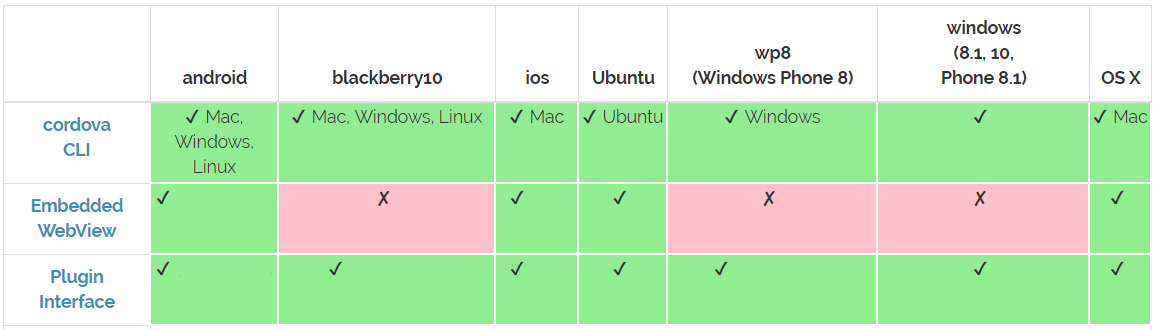
\includegraphics[width=15cm]{6-cordova-platforms}
  \caption{Bảng các nền tảng Apache Cordova hỗ trợ}\label{fig:6-cordova-platforms}
\end{figure}

\noindent
Với tính đơn giản dễ sử dụng, đồng thời có khả năng hỗ trợ nhiều nền tảng di động khác nhau được thể hiện ở \ref{fig:6-cordova-platforms}, đặc biệt là 3 nền tảng di động chính được sử dụng rộng rãi hiện nay là Android, iOS và Windows Phone, chúng tôi quyết định sử dụng công nghệ Apache Cordova để chuyển tiếp ứng dụng từ nền tảng Web sang các nền tảng di động khác nhau.

\subsection{Hiện thực ứng dụng di động}
Theo kiến trúc ứng dụng đã được trình bày ở Chương 5, ứng dụng di động sẽ bao gồm 6 trang giao diện chính (main pages) và 8 thành phần chia sẻ (shared components) là các thành phần chung được sử dụng lại nhiều lần giữa các trang giao diện khác nhau hoặc trong cùng một trang giao diện.

\subsubsection{Các thành phần chia sẻ (reusable components):}

\noindent
Các thành phần chia sẻ trong ứng dụng bao gồm 8 thành phần:

\begin{itemize}[topsep=1mm,itemsep=-0.5mm]
\item Thanh công cụ (Navbar).
\item Thẻ nhà (Home-panel).
\item Thẻ kiểu thiết bị (Device-type-panel).
\item Thẻ thiết bị (Device-panel).
\item Thẻ kịch bản (Device-script-panel).
\item Thẻ kịch bản khi/thì (Device-script-when-then).
\item Thẻ kịch bản từ/đến (Device-script-from-to).
\item Thẻ kịch bản tự tạo (Device-script-custom).
\vspace{1mm}
\end{itemize}

\noindent
Các thành phần này thực chất là các Chỉ thị (Directive) của AngularJS, với mỗi thành phần có một giao diện với một bộ quản lý (controller) đảm nhận các xử lý nghiệp vụ riêng. Vì bản chất là Chỉ thị (Directive), mỗi thành phần đều có thể dễ dàng gắn vào nhau hoặc vào các thành phần chính như là một dạng thẻ HTML bình thường.

\noindent
\underline{Thanh công cụ (Navbar)}

\noindent
Thanh công cụ (Navbar) ở hình \ref{fig:6-navbar} là thành phần chia sẻ cho phép người dùng thực hiện một số các thao tác cơ bản của ứng dụng một cách nhanh chóng, được sử dụng ở các trang giao diện chính là: danh sách các ngôi nhà, danh sách các kiểu thiết bị và danh sách các thiết bị. Thanh công cụ có nhiều chức năng khác nhau tùy thuộc vào trang giao diện chính mà nó được sử dụng. Các chức năng của thanh công cụ:

\begin{itemize}[topsep=1mm,itemsep=-0.5mm]
\item Thể hiện tên của ngôi nhà hiện tại đang truy cập.
\item Cho phép người dùng quay lại trang giao diện danh sách các Kiểu thiết bị.
\item Cho phép người dùng đăng xuất.
\item Cho phép người dùng kích hoạt các chế độ.
\item Cho phép người dùng xem, cập nhật chỉnh sửa thông tin hoặc xóa các chế độ như ở hình \ref{fig:6-EditMode}.
\vspace{1mm}
\end{itemize}

\begin{figure}[h]
  \centering
     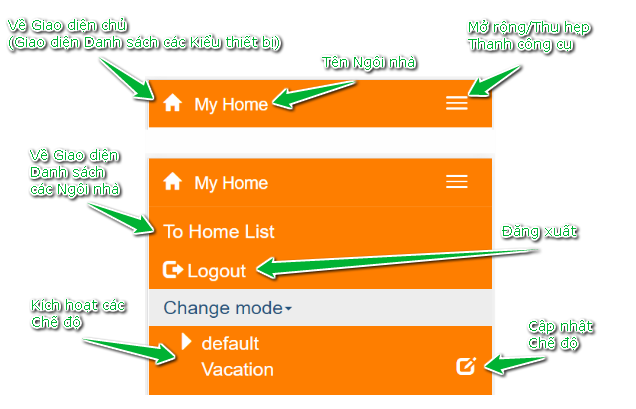
\includegraphics[width=11cm]{6-navbar}
  \caption{Thanh công cụ (Navbar)}\label{fig:6-navbar}
\end{figure}

\begin{figure}[h!]
  \centering
     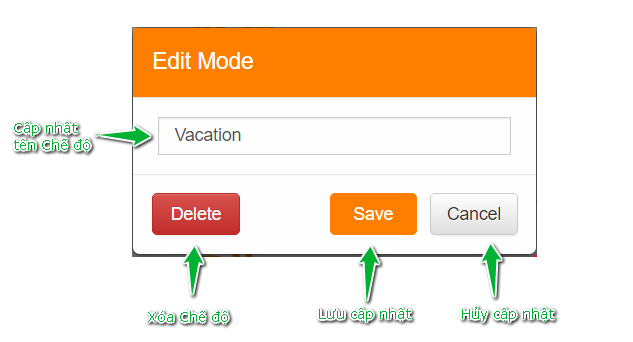
\includegraphics[width=11cm]{6-EditMode}
  \caption{Bảng hộp thoại cập nhật chế độ}\label{fig:6-EditMode}
\end{figure}

\noindent
\underline{Thẻ nhà (Home-panel)}

\noindent
Thẻ nhà (Home-panel) ở hình \ref{fig:6-home-panel} là thành phần chia sẻ thể hiện thông tin của một ngôi nhà được lắp đặt hệ thống, thành phần này được sử dụng nhiều lần như một danh sách trong trang giao diện chính danh sách các ngôi nhà. Các chức năng của thẻ nhà:

\begin{itemize}[topsep=1mm,itemsep=-0.5mm]
\item Thể hiện tên của ngôi nhà.
\item Cho phép người dùng ngưng hoạt động tạm thời (Disable) hoặc tái hoạt động (Enable) ngôi nhà.
\item Cho phép người dùng xem, cập nhật chỉnh sửa thông tin hoặc xóa ngôi nhà như ở hình \ref{fig:6-EditHome}.
\item Chuyển tiếp người dùng tới thành phần chính Danh sách các Kiểu thiết bị.
\vspace{1mm}
\end{itemize}

\begin{figure}[h]
  \centering
     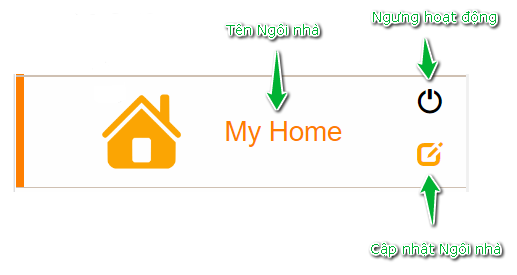
\includegraphics[width=12cm]{6-home-panel}
  \caption{Thẻ nhà}\label{fig:6-home-panel}
\end{figure}

\begin{figure}[h!]
  \centering
     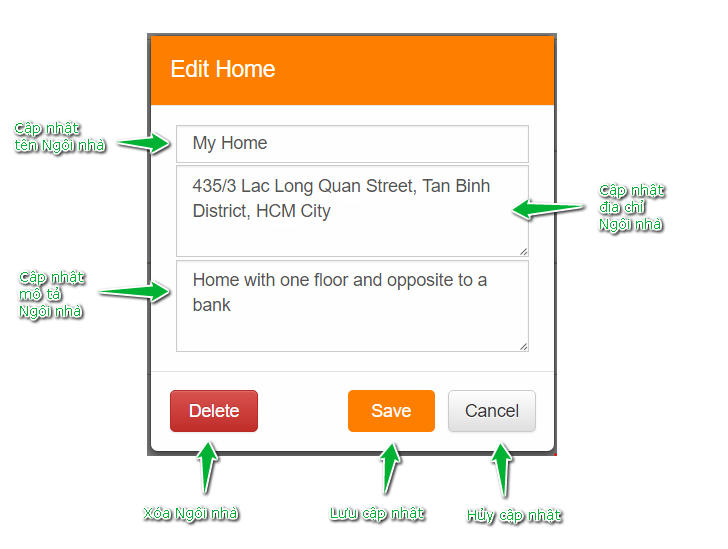
\includegraphics[width=12cm]{6-EditHome}
  \caption{Bảng hộp thoại cập nhật Ngôi nhà}\label{fig:6-EditHome}
\end{figure}

\noindent
\underline{Thẻ Kiểu thiết bị (Device-type-panel)}

\begin{figure}[h]
  \centering
     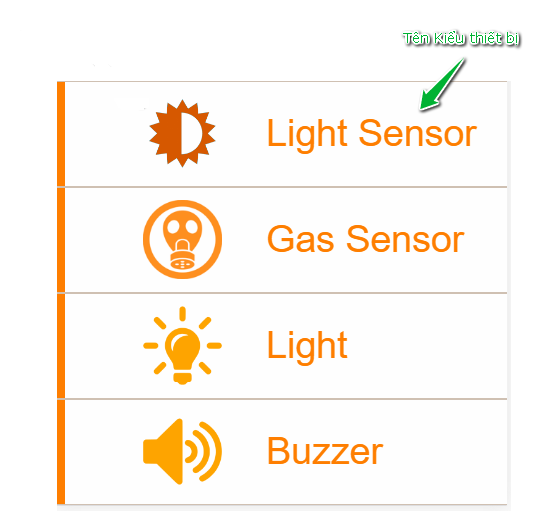
\includegraphics[width=10cm]{6-device-type-panels}
  \caption{Một số Thẻ kiểu thiết bị}\label{fig:6-device-type-panels}
\end{figure}

\noindent
Thẻ kiểu thiết bị (Device-type-panel) ở hình \ref{fig:6-device-type-panels} là thành phần đóng góp thể hiện thông tin của một kiểu thiết bị được hệ thống hỗ trợ, thành phần này được sử dụng nhiều lần như một danh sách trong thành phần chính Danh sách Các kiểu thiết bị. Ứng với mỗi kiểu thiết bị thì thẻ kiểu thiết bị có kí hiệu thể hiện và tên khác nhau, có 6 kiểu thiết bị hỗ trợ: Cảm biến nhiệt độ (Temperature Sensor), cảm biến chuyển động (Motion Sensor), cảm biến ánh sánh (Light Sensor), cảm biến khí gas (Gas Sensor), bóng đèn (Light) và còi hú (Buzzer). Các chức năng của thẻ kiểu thiết bị:

\begin{itemize}[topsep=1mm,itemsep=-0.5mm]
\item Thể hiện thông tin của kiểu thiết bị.
\item Chuyển tiếp người dùng tới trang giao diện chính danh sách các thiết bị.
\vspace{1mm}
\end{itemize}

\noindent
\underline{Thẻ Thiết bị (Device-panel)}

\begin{figure}[h]
  \centering
     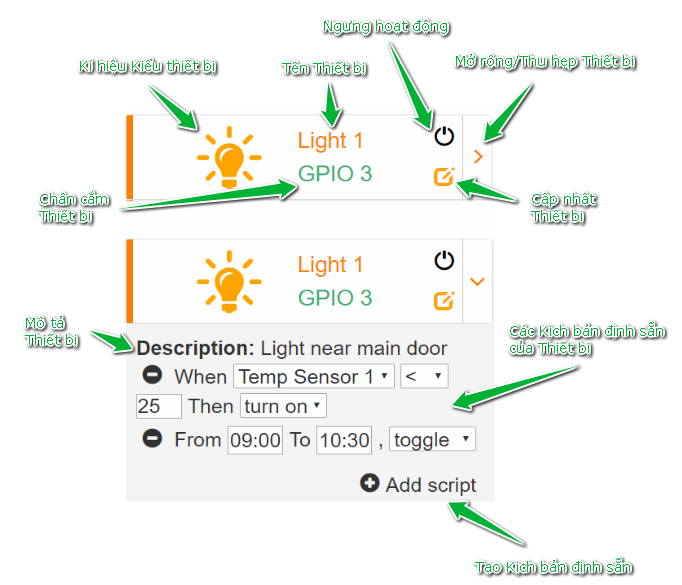
\includegraphics[width=10cm]{6-device-panel}
  \caption{Thẻ Thiết bị}\label{fig:6-device-panel}
\end{figure}

\begin{figure}[h!]
  \centering
     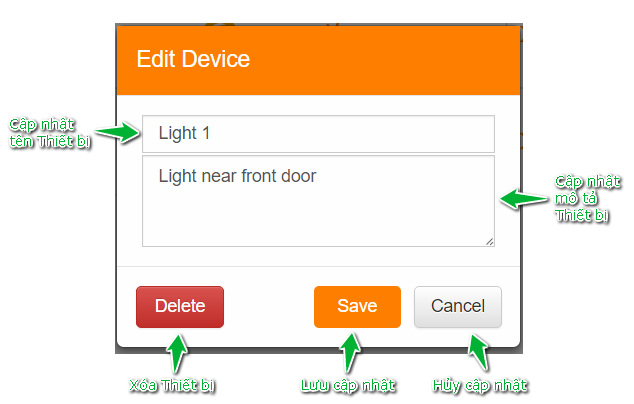
\includegraphics[width=10cm]{6-EditDevice}
  \caption{Bảng hộp thoại cập nhật Thiết bị}\label{fig:6-EditDevice}
\end{figure}

\noindent
Thẻ thiết bị (Device-panel) ở hình \ref{fig:6-device-panel} là thành phần chia sẻ thể hiện thông tin của một thiết bị cùng với các kịch bản định sẵn của thiết bị đó, được sử dụng nhiều lần như một danh sách trong trang trang giao diện danh sách các thiết bị. Thành phần này chứa bên trong nó một tập hợp các thành phần chia sẻ thẻ kịch bản để hỗ trợ việc thể hiện thông tin các Kịch bản thuộc thiết bị. Các chức năng của thẻ thiết bị:

\begin{itemize}[topsep=1mm,itemsep=-0.5mm]
\item Thể hiện kiểu, tên và chân cắm của thiết bị.
\item Cho phép người dùng ngưng hoạt động tạm thời (Disable) hoặc tái hoạt động (Enable) thiết bị.
\item Cho phép người dùng xem, cập nhật chỉnh sửa thông tin hoặc xóa thiết bị như ở hình \ref{fig:6-EditDevice}
\item Cho phép người dùng xem thông tin các kịch bản định sẵn của thiết bị.
\item Cho phép người dùng tạo thêm kịch bản định sẵn cho thiết bị.
\vspace{1mm}
\end{itemize}

\noindent
\underline{Thẻ kịch bản (Device-script-panel)}

\noindent
Thẻ kịch bản (Device-script-panel) chứa bên trong nó 3 thành phần đóng góp khác là thẻ Kịch bản khi/thì (Device-script-when-then), thẻ Kịch bản từ/đến (Device-script-from-to) và thẻ Kịch bản tự tạo (Device-script-custom). Tùy vào loại tịch bản được truyền vào mà thành phần này sẽ quyết định lựa chọn một trong 3 thành phần đóng góp bên trong nó để thể hiện.

\noindent
\underline{Thẻ Kịch bản khi/thì (Device-script-when-then)}

\begin{figure}[h]
  \centering
     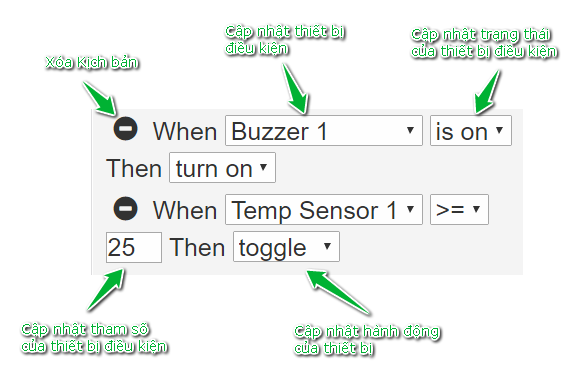
\includegraphics[width=10cm]{6-device-script-when-then}
  \caption{Một số Thẻ Kịch bản khi/thì}\label{fig:6-device-script-when-then}
\end{figure}

\noindent
Thẻ kịch bản khi/thì (Device-script-when-then) ở hình \ref{fig:6-device-script-when-then} là thành phần chia sẻ thể hiện thông tin của một kịch bản thuộc loại khi/thì (When/Then), với 2 bộ phận là điều kiện và hành động. Bộ phận điều kiện gồm 3 bộ phận nhỏ hơn là thiết bị điều kiện, trạng thái của thiết bị điều kiện và tham số của thiết bị điều kiện. Tham số của thiết bị điều kiện có được thể hiện hay không tùy thuộc vào kiểu của thiết bị điều kiện. Các chức năng của thẻ kịch bản khi/thì:

\begin{itemize}[topsep=1mm,itemsep=-0.5mm]
\item Thể hiện nội dung bao gồm điều kiện và hành động của kịch bản thuộc loại khi/thì.
\item Cho phép người dùng cập nhật chỉnh sửa thiết bị điều kiện.
\item Cho phép người dùng cập nhật chỉnh sửa trạng thái của thiết bị điều kiện.
\item Cho phép người dùng cập nhật chỉnh sửa tham số của thiết bị điều kiện.
\item Cho phép người dùng cập nhật chỉnh sửa hành động của thiết bị.
\item Cho phép người dùng xóa kịch bản.
\vspace{1mm}
\end{itemize}

\noindent
\underline{Thẻ kịch bản từ/đến (Device-script-from-to)}

\begin{figure}[h]
  \centering
     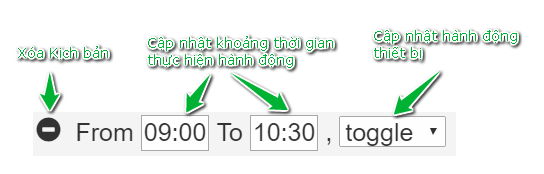
\includegraphics[width=10cm]{6-device-script-from-to}
  \caption{Thẻ Kịch bản từ/đến}\label{fig:6-device-script-from-to}
\end{figure}

\noindent
Thẻ kịch bản từ/đến (Device-script-from-to) ở hình \ref{fig:6-device-script-from-to} là thành phần chia sẻ thể hiện thông tin của một kịch bản thuộc loại từ/đến (From/To), với 2 bộ phận là khoảng thời gian hành động được thực hiện và hành động. Các chức năng của thẻ kịch bản từ/đến:

\begin{itemize}[topsep=1mm,itemsep=-0.5mm]
\item Thể hiện nội dung bao gồm khoảng thời gian hành động được thực hiện và hành động của kịch bản thuộc loại từ/đến.
\item Cho phép người dùng cập nhật chỉnh sửa khoảng thời gian thực hiện hành động của thiết bị.
\item Cho phép người dùng cập nhật chỉnh sửa hành động của thiết bị.
\item Cho phép người dùng xóa kịch bản.
\vspace{1mm}
\end{itemize}

\noindent
\underline{Thẻ kịch bản tự tạo (Device-script-custom)}

\begin{figure}[h]
  \centering
     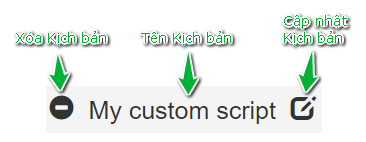
\includegraphics[width=10cm]{6-DeviceScriptCustom}
  \caption{Thẻ Kịch bản tự tạo}\label{fig:6-DeviceScriptCustom}
\end{figure}

\begin{figure}[h]
  \centering
     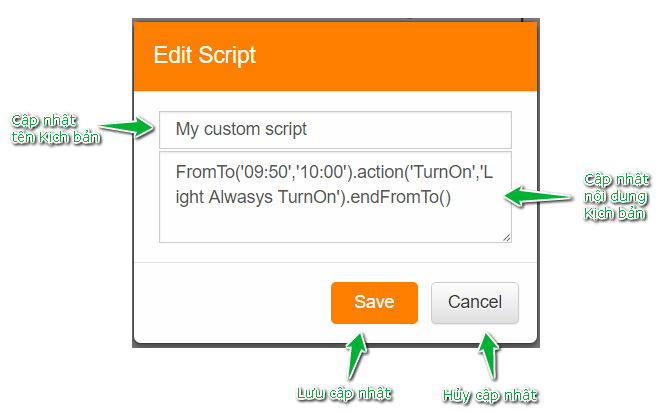
\includegraphics[width=10cm]{6-EditCustomScript}
  \caption{Bảng hộp thoại cập nhật Kịch bản tự tạo}\label{fig:6-EditCustomScript}
\end{figure}

\noindent
Thẻ kịch bản tự tạo (Device-script-custom) ở hình \ref{fig:6-DeviceScriptCustom} là thành phần chia sẻ thể hiện thông tin của một kịch bản tự tạo, với khả năng tùy biến nội dung kịch bản phức tạp cần nhiều thiết bị, điều kiện và hành động. Thành phần này gồm 2 bộ phận là tên kịch bản và nội dung kịch bản. Các chức năng của thẻ kịch bản tự tạo:

\begin{itemize}[topsep=1mm,itemsep=-0.5mm]
\item Thể hiện tên của kịch bản tự tạo.
\item Cho phép người dùng cập nhật chỉnh sửa tên và nội dung của kịch bản như ở hình \ref{fig:6-EditCustomScript}.
\item Cho phép người dùng xóa kịch bản.
\vspace{1mm}
\end{itemize}

\subsubsection{Các trang giao diện chính (main pages)}

\noindent
Các trang giao diện chính trong ứng dụng bao gồm 6 trang:

\begin{itemize}[topsep=1mm,itemsep=-0.5mm]
\item Trang đăng nhập (Login Page).
\item Trang đăng ký (Registration Page).
\item Trang danh sách các ngôi nhà (Home List Page).
\item Trang danh sách các kiểu thiết bị (Device Category List Page).
\item Trang danh sách các thiết bị (Device List Page).
\item Trang danh sách các kịch bản tự tạo (Custom Script List Page).
\vspace{1mm}
\end{itemize}

\noindent
Các trang giao diện chính này là các trang HTML, với mỗi trang có một bộ quản lý (controller) của AngularJS đảm nhận các xử lý nghiệp vụ riêng.

\noindent
\underline{Trang đăng nhập (Login Page)}

\begin{figure}[h]
  \centering
     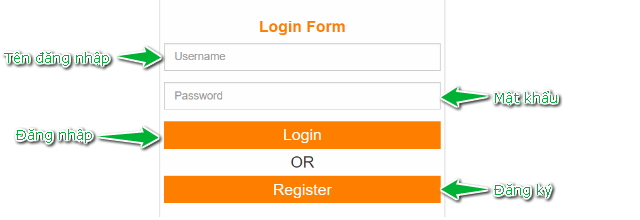
\includegraphics[width=10cm]{6-LoginPage}
  \caption{Trang đăng nhập}\label{fig:6-LoginPage}
\end{figure}

\noindent
Trang đăng nhập (Login Page) ở hình \ref{fig:6-LoginPage} là trang giao diện đầu tiên người dùng truy cập khi sử dụng ứng dụng, cung cấp giao diện đơn giản để người dùng thực hiện thao tác đăng nhập vào ứng dụng. Các chức năng chính của trang đăng nhập:

\begin{itemize}[topsep=1mm,itemsep=-0.5mm]
\item Cho phép người dùng đăng nhập vào ứng dụng với tên đăng nhập và mật khẩu.
\item Chuyển tiếp người dùng đến trang đăng ký.
\item Chuyển tiếp người dùng đến trang danh sách các ngôi nhà.
\vspace{1mm}
\end{itemize}

\noindent
\underline{Trang đăng ký (Registration Page)}

\begin{figure}[h]
  \centering
     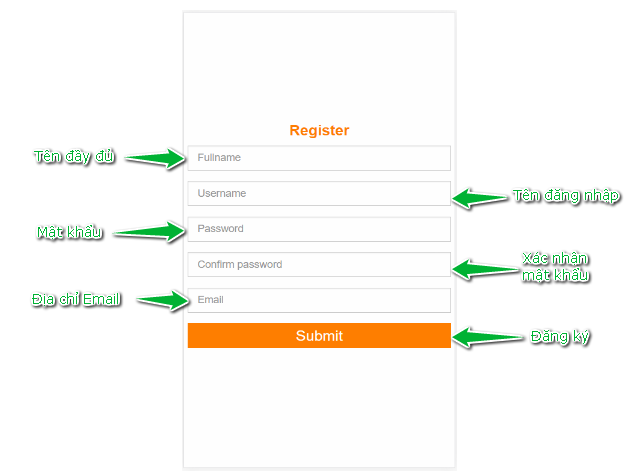
\includegraphics[width=10cm]{6-RegisterPage}
  \caption{Trang đăng ký}\label{fig:6-RegisterPage}
\end{figure}

\noindent
Trang đăng ký (Registration Page) ở hình \ref{fig:6-RegisterPage} cung cấp giao diện đơn giản để người dùng thực hiện thao tác đăng ký vào ứng dụng. Khi đăng ký với các thông tin hợp lệ, ứng dụng sẽ gửi một Email tới địa chỉ Email đã nhập của người dùng để xác nhận thông tin đăng ký. Các chức năng chính của trang đăng ký:

\begin{itemize}[topsep=1mm,itemsep=-0.5mm]
\item Cho phép người dùng đăng ký sử dụng ứng dụng với tên đầy đủ, tên đăng nhập, mật khẩu và địa chỉ Email.
\item Chuyển tiếp người dùng về trang đăng nhập.
\vspace{1mm}
\end{itemize}

\noindent
\underline{Trang danh sách các ngôi nhà (Home List Page)}

\begin{figure}[h]
  \centering
     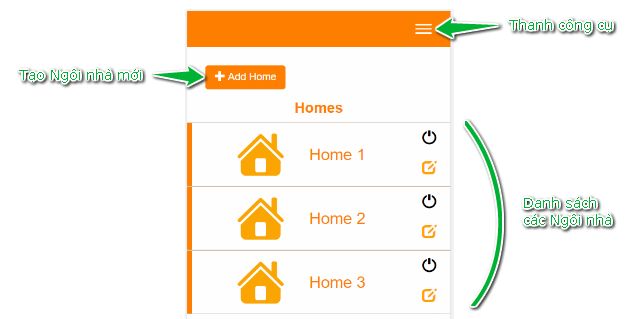
\includegraphics[width=10cm]{6-HomeListPage}
  \caption{Trang danh sách các ngôi nhà}\label{fig:6-HomeListPage}
\end{figure}

\begin{figure}[h!]
  \centering
     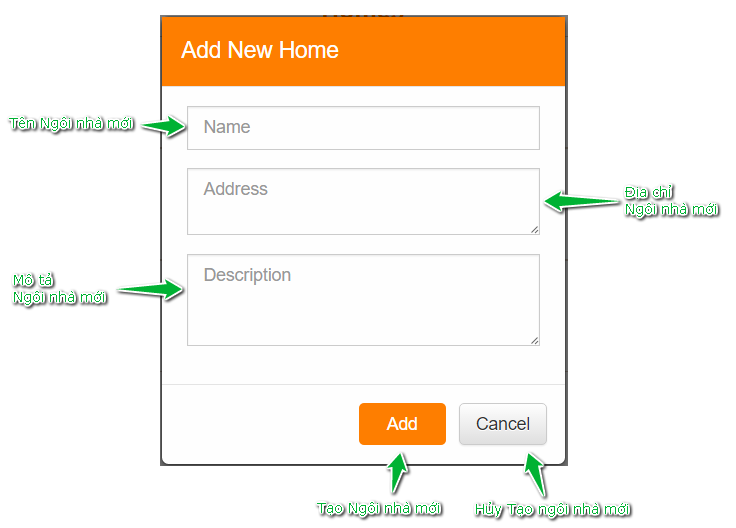
\includegraphics[width=10cm]{6-AddHome}
  \caption{Bảng hộp thoại tạo ngôi nhà mới}\label{fig:6-AddHome}
\end{figure}

\noindent
Trang danh sách các ngôi nhà (Home List Page) ở hình \ref{fig:6-HomeListPage} cung cấp giao diện để người dùng xem thông tin, quản lý và tạo mới các ngôi nhà được lắp đặt hệ thống. Trang giao diện này sử dụng các thành phần chia sẻ là thanh công cụ và thẻ nhà để thể hiện thông tin. Các chức năng chính của trang danh sách các ngôi nhà:

\begin{itemize}[topsep=1mm,itemsep=-0.5mm]
\item Thể hiện thông tin danh sách các ngôi nhà của người dùng.
\item Cho phép người dùng tạo mới một ngôi nhà như ờ hình \ref{fig:6-AddHome}.
\item Chuyển tiếp người dùng đến trang danh sách các kiểu thiết bị.
\vspace{1mm}
\end{itemize}

\noindent
\underline{Trang danh sách các kiểu thiết bị (Device Category List Page)}

\begin{figure}[h]
  \centering
     \includegraphics[width=10cm]{6-DeviceCategoryList}
  \caption{Trang danh sách các kiểu thiết bị}\label{fig:6-DeviceCategoryList}
\end{figure}

\begin{figure}[h]
  \centering
     \includegraphics[width=10cm]{6-AddMode}
  \caption{Bảng hộp thoại tạo chế độ mới}\label{fig:6-AddMode}
\end{figure}

\noindent
Trang danh sách các kiểu thiết bị (Device Category List Page) ở hình \ref{fig:6-DeviceCategoryList} cung cấp giao diện để người dùng xem thông tin các kiểu thiết bị, đồng thời kích hoạt, tạo mới và chuyển đổi các chế độ hiển thị. Trang giao diện này sử dụng các thành phần đóng góp là thanh công cụ và thẻ Kiểu thiết bị để thể hiện thông tin. Các chức năng chính của trang danh sách các kiểu thiết bị:

\begin{itemize}[topsep=1mm,itemsep=-0.5mm]
\item Thể hiện thông tin danh sách các kiểu thiết bị mà ứng dụng hỗ trợ.
\item Cho phép người dùng chuyển đổi chế độ hiển thị.
\item Cho phép người dùng kích hoạt một chế độ.

\item Cho phép người dùng tạo mới một chế độ như ở hình \ref{fig:6-AddMode}.
\item Chuyển tiếp người dùng đến trang danh sách các thiết bị.
\item Chuyển tiếp người dùng đến trang danh sách các kịch bản tự tạo.
\vspace{1mm}
\end{itemize}

\noindent
\underline{Trang danh sách các thiết bị (Device List Page)}

\begin{figure}[h]
  \centering
     \includegraphics[width=10cm]{6-DeviceListPage}
  \caption{Trang danh sách các thiết bị}\label{fig:6-DeviceListPage}
\end{figure}

\begin{figure}[h!]
  \centering
     \includegraphics[width=10cm]{6-AddDevice}
  \caption{Bảng hộp thoại tạo thiết bị mới}\label{fig:6-AddDevice}
\end{figure}

\noindent
Trang danh sách các thiết bị (Device List Page) ở hình \ref{fig:6-DeviceListPage} cung cấp giao diện để người dùng xem thông tin, quản lý và tạo mới các thiết bị. Trang giao diện này sử dụng các thành phần đóng góp là thanh công cụ và thẻ thiết bị để thể hiện thông tin. Các chức năng chính của trang danh sách các thiết bị:

\begin{itemize}[topsep=1mm,itemsep=-0.5mm]
\item Thể hiện thông tin danh sách các thiết bị thuộc một kiểu thiết bị của người dùng.
\item Cho phép người dùng tạo mới một thiết bị như ở hình \ref{fig:6-AddDevice}.
\vspace{1mm}
\end{itemize}

\noindent
\underline{Trang danh sách các kịch bản tự tạo (Custom Script List Page)}

\begin{figure}[h]
  \centering
     \includegraphics[width=10cm]{6-CustomScriptList}
  \caption{Trang danh sách các kịch bản tự tạo}\label{fig:6-CustomScriptList}
\end{figure}

\begin{figure}[h]
  \centering
     \includegraphics[width=10cm]{6-AddCustomScript}
  \caption{Bảng hộp thoại tạo kịch bản tự tạo mới}\label{fig:6-AddCustomScript}
\end{figure}

\noindent
Trang danh sách các kịch bản tự tạo (Custom Script List Page) ở hình \ref{fig:6-CustomScriptList} cung cấp giao diện để người dùng xem thông tin, quản lý và tạo mới các kịch bản tự tạo. Trang giao diện này sử dụng các thành phần đóng góp là thanh công cụ và thẻ Kịch bản tư tạo để thể hiện thông tin. Các chức năng chính của trang danh sách các kịch bản tự tạo:

\begin{itemize}[topsep=1mm,itemsep=-0.5mm]
\item Thể hiện thông tin danh sách các kịch bản tự tạo của người dùng.
\item Cho phép người dùng tạo mới một kịch bản tự tạo như ở hình \ref{fig:6-AddCustomScript}.
\vspace{1mm}
\end{itemize}

\noindent
Với việc hiện thực 6 trang giao diện chính cùng các thành phần chia sẻ như trên, ứng dụng di động cung cấp đầy đủ các chức năng cần thiết để người dùng có thể dễ dàng quản lý các ngôi nhà, thiết bị và kịch bản của hệ thống cũng như phản ánh được kiến trúc tổng quát đã được trình bày ở Chương 5.

%-----------------------------------
\chapter{Thí nghiệm và đánh giá hệ thống}
\section{Phương pháp thực nghiệm}

Nhóm tiến hành lắp đặt lần lượt các thiết bị gồm: cảm biến nhiệt, cảm biến ánh sáng, cảm biến khí gas, cảm biến chuyển động, đèn và còi hú vào Raspberry Pi. Hình \ref{fig:7-real-system} mô tả thiết bị demo của nhóm được gắn trên Raspberry Pi. Sau đó, nhóm cho thiết bị mobile cùng Raspberry Pi kết nối đến cùng 1 mạng local qua sử dụng máy tính làm Wifi hotspot. Nhóm tiến hành đăng ký thông qua giao diện ứng dụng và tạo mới nhà, tạo mới chế độ, thiết bị, thêm kịch bản. Một vài kịch bản mà nhóm chuẩn bị cho thí nghiệm.

\begin{figure}[h]
  \centering
     \includegraphics[width=15cm]{7-real-system}
  \caption{Mô hình thí nghiệm thực tế}\label{fig:7-real-system}
\end{figure}

\noindent
Chế độ 1 (kiểm tra cảm biến ánh sáng):

\begin{itemize}[topsep=1mm,itemsep=-0.5mm]
\item Nếu cảm biến ánh sáng phát hiện xung quanh sáng thì đèn tắt.
\item Nếu cảm biến ánh sáng phát hiện xung quanh tối thì đèn bật.
\vspace{1mm}
\end{itemize}

\noindent
Chế độ 2 (kiểm tra cảm biến khí gas):

\begin{itemize}[topsep=1mm,itemsep=-0.5mm]
\item Nếu cảm biến khí gas phát hiện nồng độ gas vượt quá một ngưỡng cho phép (có thể điều chỉnh thông qua cảm biến khí gas) thì còi hú.
\item Nếu cảm biến khí gas phát hiện nồng độ gas ở mức bình thường thì còi tắt.
\item Chuẩn bị kịch bản có khả năng mâu thuẫn: Trong khoảng 19h00 đến 20h00 thì còi tắt.
\vspace{1mm}
\end{itemize}

\noindent
Chế độ 3 (kịch bản thời gian):

\begin{itemize}[topsep=1mm,itemsep=-0.5mm]
\item Trong khoảng thời gian từ 18h00 đến 22h00 thì đèn bật.
\item Trong khoảng thời gian từ 22h01 đến 17h59 thì đèn tắt.
\item Chuẩn bị kịch bản mâu thuẫn: Trong khoảng 19h00 đến 20h00 thì đèn tắt.
\vspace{1mm}
\end{itemize}

\noindent
Chế độ 4 (nhiều kịch bản phối hợp):

\begin{itemize}[topsep=1mm,itemsep=-0.5mm]
\item Nếu nhiệt độ thu được từ cảm biến nhiệt lớn hơn 31 độ thì đèn bật.
\item Nếu nhiệt độ thu được từ cảm biến nhiệt bé hơn 31 độ thì đèn tắt.
\item Nếu đèn bật thì còi hú.
\item Nếu đèn tắt thì còi tắt.
\vspace{1mm}
\end{itemize}

\noindent
Chế độ 5 (kiểm tra cảm biến chuyển động cùng phối hợp kịch bản thời gian):

\begin{itemize}[topsep=1mm,itemsep=-0.5mm]
\item Nếu phát hiện vật thể chuyển động thì đèn bật và nếu trong khoảng thời gian từ 22h00 đến 06h00 thì còi hú.
\item Nếu không còn phát hiện vật thể chuyển động nữa thì đèn và còi tắt.
\vspace{1mm}
\end{itemize}

\noindent
Chế độ 6 (kịch bản phức tạp):

\noindent
\hspace{1.2cm} \textbf{Nếu} (cảm biến ánh sáng phát hiện xung quanh tối) \textbf{thì}

\hspace{2cm}(bật đèn và nếu (phát hiện khí gas) \textbf{thì}

\hspace{3cm}(đồng thời tắt đèn, mở còi hú)\

\hspace{3cm}hoặc không mà trong thời gian \textbf{từ} 09h00 \textbf{đến} 14h00 \textbf{thì}

\hspace{3cm}(tắt đèn và tắt còi)

\noindent\hspace{2cm} )\\

\noindent
Ngôi nhà sẽ có lần lượt 5 chế độ với các kịch bản dành cho các thiết bị như trên. Việc đánh giá hệ thống được thực hiện thủ công bằng cách so sánh kết quả mong đợi từ kịch bản với kết quả thực tế quan sát thông qua thiết bị trong cùng điều kiện. Ngoài ra, nhóm còn thực hiện unit test cho việc kiểm tra kịch bản hợp lệ (trùng tên, kịch bản mâu thuẫn, kịch bản có khả năng mâu thuẫn, kịch bản trùng nội dung nhưng đảo thứ tự điều kiện, hành động,\dots).

\section{Kết quả và đánh giá}

Sau khi tiến hành các thực nghiệm trên, nhóm rút ra một số đánh giá sơ bộ về hệ thống:

\begin{itemize}[topsep=1mm,itemsep=-0.5mm]
\item Các thiết bị hoạt động tốt với Raspberry Pi.
\item Với hầu hết các kịch bản mô tả từ đơn giản đến phức tạp thì hệ thống vẫn có thể xử lý tốt, chạy đúng kết quả mong muốn (ví dụ như các kịch bản ở phần thực nghiệm trên) miễn rằng nó là kịch bản hợp lệ.
\item Việc kiểm tra các kịch bản mâu thuẫn, có khả năng mâu thuẫn để loại trừ ra khỏi hệ thống hoạt động ổn định và tốt.
\item Hệ thống hỗ trợ bảo mật tài khoản người dùng, bảo mật tài nguyên hệ thống (chỉ có người dùng sở hữu ngôi nhà mới được truy xuất đến các tài nguyên thuộc nhà ấy).
\item Khi thực hiện việc vô hiệu hóa (disable) ngôi nhà, hay thiết bị thì các kịch bản lần lượt thuộc nhà và thiết bị ấy sẽ vào trạng thái dừng như mong đợi. Cũng như thực hiện thao tác kích hoạt (enable) nhà, thiết bị trở lại thì kịch bản sẽ chạy lại như bình thường.
\item Giao diện ứng dụng đơn giản, cung cấp nhiều chức năng cho người dùng thao tác, chỉnh sửa và xem thông tin về ngôi nhà và các thiết bị, kịch bản trong nó. Ngoài ra, ứng dụng cho phép tạo nhanh kịch bản với vài mẫu đơn giản.
\vspace{1mm}
\end{itemize}

\noindent
Tuy nhiên, còn một số khó khăn mà hệ thống đang gặp phải:

\begin{itemize}[topsep=1mm,itemsep=-0.5mm]
\item Giao diện chưa hỗ trợ tối đa người dùng trong việc xây dựng các kịch bản tùy ý (custom).
\item Trải nghiệm người dùng chưa thực sự tốt với thời gian phản hồi hệ thống còn khá cao.
\item Các mẫu kịch bản hỗ trợ sẵn còn ít, chưa thỏa mãn được nhiều nhu cầu thực tế người dùng.
\item Khi số lượng kịch bản tăng lên (tầm 30-35) thì hiệu năng hệ thống giảm đi khá nhiều, do máy tính Raspberry Pi có bộ nhớ khá “khiêm tốn” và việc quản lý kịch bản chưa thực sự tốt.
\vspace{1mm}
\end{itemize}

%------------------------------------

\chapter{Thảo luận}
\section{Giải pháp xử lý các kịch bản có khả năng mâu thuẫn}

Tại thời điểm viết luận văn này, các kịch bản có khả năng mâu thuẫn sẽ không được phép tồn tại trong hệ thống. Nhóm muốn đề xuất một phương pháp có thể xử lý tình huống này khi mở rộng hệ thống trong tương lai, đó là cho phép người dùng thiết lập thêm độ ưu tiên cho kịch bản trong trường hợp có khả năng mâu thuẫn. Giả sử trong một điều kiện nào đó, 2 kịch bản có khả năng mâu thuẫn thực sự mâu thuẫn nhau, ta hoàn toàn có thể dựa trên độ ưu tiên để xem xét kịch bản nào được chạy trong trường hợp trên, bằng cách chọn ra kịch bản có độ ưu tiên cao hơn. Tuy nhiên trong điều kiện bình thường, việc xét độ ưu tiên khi tạo ra một kịch bản mới có thể không mang lại nhiều ý nghĩa và khiến người dùng bị rối. Đứng từ khía cạnh người dùng, hệ thống có thể được xem là thông minh hơn nếu như có khả năng tự thiết lập một độ ưu tiên mặc định cho một số dạng kịch bản, dựa trên ý nghĩa, nhu cầu thực tế của kịch bản đó. Người dùng có thể tự do thay đổi giá trị mặc định đó dựa trên mục đích riêng của họ.

\subsection{Độ ưu tiên mặc định cho một số loại kịch bản }

Sau khi tham khảo từ một số nhu cầu thực tế, nhóm đề xuất ra một số dạng kịch bản có thể được xét giá trị ưu tiên mặc định. Nếu như kịch bản chứa một trong những điều kiện thuộc dạng khẩn cấp sau thì chúng lần lượt có thứ tự ưu tiên như sau (số thứ tự càng thấp thì độ ưu tiên càng cao):

\begin{enumerate}[topsep=1mm,itemsep=-0.5mm]
\item Temperature > N (N là một giá trị nào đó).
\item Phát hiện có gas.
\item Phát hiện người chuyển động trong thời gian đêm khuya.
\item Các dạng kịch bản khác.
\vspace{1mm}
\end{enumerate}

\noindent
Có thể giải thích cho việc đưa ra quyết định trên như sau:

\begin{itemize}[topsep=1mm,itemsep=-0.5mm]
\item Nếu nhiệt độ vượt ngưỡng => Khả năng có cháy xảy ra cao, dẫn đến độ nguy hiểm tính mạng cao => Ưu tiên số 1.
\item Trường hợp có gas, tức có khả năng xảy ra cháy, nhưng thật sự vẫn chưa cháy => Ưu tiên số 2.
\item Trường hợp này có khả năng là trộm => dẫn đến có thể bị mất đồ nhưng khả năng gây chết người thấp => Ưu tiên số 3.
\vspace{1mm}
\end{itemize}

\noindent
Nếu kịch bản có chứa nhiều điều kiện dạng trên thì độ ưu tiên mặc định của kịch bản ấy chỉnh là độ ưu tiên cao nhất của một trong các điều kiện liệt kê ở trên.

\subsection{Cách xử lý một số trường hợp trùng độ ưu tiên}

Như đã thảo luận ở mục trên, việc xử lý kịch bản có khả năng mâu thuẫn có thể giải quyết bằng độ ưu tiên. Nhưng một số trường hợp, chúng có cùng độ ưu tiên (người dùng không có ý muốn thay đổi độ ưu tiên mặc định) thì ta phải xử lý ra sao? Nhóm xin liệt kê và giải thích qua một vài ví dụ.

\noindent
Ví dụ 1:

\begin{itemize}[topsep=1mm,itemsep=-0.5mm]
\item Kịch bản 1: Nếu có gas thì tắt đèn phòng.
\item Kịch bản 2: Nếu có gas thì bật còi hú gần cửa ra vào và đồng thời kiểm tra nếu cảm biến ánh sáng cho kết quả bây giờ là ban ngày thì bật đèn phòng.
\vspace{1mm}
\end{itemize}

\noindent
Nhìn sơ qua, 2 kịch bản trên có khả năng mâu thuẫn nhau và đang có cùng độ ưu tiên mặc định là 2. Trường hợp này, nhóm đề xuất nếu như kịch bản nào có độ chi tiết hơn thì nó sẽ được xem là có độ “ưu tiên” cao hơn. Lý do là vì đứng từ góc nhìn người đặt ra kịch bản, việc thực thi 1 kịch bản có mức chi tiết hơn sẽ đáp ứng mong đợi người dùng nhiều hơn.

\noindent
Ví dụ 2:

\begin{itemize}[topsep=1mm,itemsep=-0.5mm]
\item Kịch bản 1: Từ 22h đến 6h thì tắt đèn phòng.
\item Kịch bản 2: Từ 5h đến 7h thì bật đèn phòng.
\vspace{1mm}
\end{itemize}

\noindent
Trường hợp này, nhóm đề xuất kịch bản 2 có độ ưu tiên cao hơn. Có thể giải thích rằng là do kịch bản bật đèn từ 5h đến 7h có khoảng giá trị nhỏ hơn từ 22h -> 6h, mang nghĩa kịch bản 2 có mức độ xuất hiện không thường xuyên cao hơn kịch bản 1 cho nên có ưu tiên cao hơn.\\

\noindent
Nếu xảy ra một trường hợp khác không nằm trong các trường hợp liệt kê mục này, hệ thống có thể thông báo cho người dùng, yêu cầu họ nhập giá trị ưu tiên cho các kịch bản có khả năng mâu thuẫn trên.

\section{Giải pháp tối ưu việc quản lý, vận hành các kịch bản dựa trên kĩ thuật multi-threading}

Kịch bản là một khái niệm quan trọng trong hệ thống này. Như ta đã biết, kịch bản được tạo ra, được hệ thống chuyển đổi, kiểm tra hợp lệ,\dots\hspace{0mm} và cuối cùng là chạy nó. Với thiết kế hệ thống hiện tại, mỗi kịch bản được quản lý bởi 1 thread riêng biệt. Khi kịch bản ở trạng thái chạy, cứ cách một khoảng thời gian ngắn, kịch bản ấy sẽ được kiểm tra lại điều kiện và thực thi hành động tương ứng, điều đó diễn ra thành vòng lặp vô tận. Có thể để ý thấy, mỗi thread không luôn luôn phải ở trạng thái sẵn sàng (active) mà nó chỉ cần hoạt động sau mỗi khoảng thời gian ngắn. Từ đó dẫn đến việc lãng phí một lượng lớn tài nguyên hệ thống (ở đây là lãng phí xử lý CPU và cả bộ nhớ, memory) chỉ phục vụ cho mục đích chờ đợi là chủ yếu. Thử tưởng tượng nếu hệ thống có tầm 20 kịch bản, đồng nghĩa có 20 threads tại thời điểm này, trong khi bộ nhớ của Rapsberry Pi khá thấp, CPU cũng không đủ mạnh, việc xử lý đa luồng và mỗi luồng là một kịch bản có thể sẽ làm giảm hiệu năng toàn hệ thống.\\

\noindent
Sau thời gian tìm hiểu và thảo luận, nhóm xin đề xuất một thuật toán cải tiến nhỏ giúp cho việc quản lý trên hiệu quả hơn. Ta sẽ vẫn giữ mỗi thread quản lý một kịch bản, tuy nhiên điểm khác biệt đó là việc chạy kịch bản chỉ được thực hiện 1 lần khi tạo, hay 1 lần sau khi cập nhật mới nội dung kịch bản. Trong module “Scenario Runner”, ta hiện thực thêm 1 hashmap “scenario mapping” chả hạn, để ánh xạ kịch bản với thread quản lý nó. Nếu như có bất kì thay đổi nào tới kịch bản, dựa trên hashmap “scenario mapping” trên để thông báo đến thread tương ứng và chạy lại kịch bản mới ấy. Với cách hiện thực này, việc lãng phí tài nguyên CPU sẽ giảm đi đáng kể và chỉ còn chi phí khi lưu thread trên bộ nhớ thôi.

\section{Giải pháp xây dựng hệ thống ứng dụng điện toán đám mây phục vụ nhiều người dùng}

Trong luận văn này, ứng dụng hệ thống chỉ dừng lại ở mức demo với các thiết bị đơn giản và mọi dịch vụ được cung cấp bởi Raspberry Pi. Tuy nhiên, khi hệ thống này đươc áp dụng vào thực tế, nhóm đề xuất sẽ đưa các dịch vụ lên trên đám mây (cloud). Cụ thể, ta sẽ có 1 cloud server, cung cấp các dịch vụ liên quan việc quản lý thông tin các ngôi nhà, chế độ, thiết bị, kịch bản người dùng và cả Raspeberry Pi trong nhà.\\

\begin{figure}[h]
  \centering
     \includegraphics[width=15cm]{6-Communicate-among-client-server-and-Pi}
  \caption{Cách thức giao tiếp giữa client, server và Raspberry Pi}\label{fig:6-Communicate-among-client-server-and-Pi}
\end{figure}

\noindent
Hình \ref{fig:6-Communicate-among-client-server-and-Pi} mô tả cách giao tiếp giữa người dùng, Pi và cloud server. Khi người dùng đăng ký sử dụng dịch vụ của hệ thống, họ sẽ được cấp 1 con Pi với mã code do ta quy định và được lưu trên cloud. Sau đó, người dùng được trợ giúp lắp đặt thiết bị vào con Pi đó và tiến hành đăng ký với hệ thống (thông qua giao diện ứng dụng) để xác nhận việc muốn gắn Pi vào ngôi nhà của mình. Hệ thống nhận được yêu cầu đăng kí và dựa trên mã code gửi kèm sẽ kích hoạt con Pi có mã tương ứng. Kể từ lúc này, thông qua giao diện ứng dụng, người dùng có thể thêm nhà, thiết bị, kịch bản,\dots\hspace{0mm} Mọi thông tin này được lưu trữ và quản lý trên cloud. Raspberry Pi sau khi đã kích hoạt cũng sẽ kết nối với cloud và nhận các thông tin về kịch bản gửi từ cloud server. Nhiệm vụ của Pi giờ chỉ là thực thi những kịch bản đó cùng với việc điều khiển các thiết bị theo như kịch bản đã định.

%-------------------------------------Tổng kết----------------------------------%
\chapter{Tổng kết}

Với mục tiêu của đề tài “Xây dựng hệ thống nhà thông minh sử dụng Raspberry Pi” là hướng tới phát triển một hệ thống điều khiển các thiết bị thông dụng trong nhà thông qua các kịch bản người dùng mong muốn một cách dễ dàng và tiện lợi, chúng tôi đã tìm hiểu được cách thức hoạt động và điều khiển các thiết bị phần cứng được gắn trên máy tính kích thước nhỏ Raspberry Pi, hiện thực một máy chủ với vai trò xử lý các kịch bản của người dùng và một ứng dụng di động cho phép người dùng dễ dàng truy cập và quản lý các thiết bị.\\

\noindent
Về mặt các thiết bị hỗ trợ, chúng tôi đã triển khai việc lắp đặt và điều khiển thành công các thiết bị: Bóng đèn, còi hú, cảm biến nhiệt độ, cảm biến chuyển động, cảm biến ánh sáng và cảm biến khí gas vào Raspberry Pi. Tuy nhiên, việc điều khiển các thiết bị thông qua Raspberry Pi vẫn còn nhiều hạn chế như số lượng giới hạn các cổng GPIO, phải điều chỉnh độ nhạy của các cảm biến bằng tay, không xác định một cách tự động loại thiết bị được gắn vào chân GPIO,\dots\hspace{0mm} Vì mục tiêu đề tài hướng trọng tâm vào việc xử lý các tác vụ trên phương diện phần mềm, nên việc lặp đặt các thiết bị phần cứng vẫn còn dừng ở mức thí nghiệm, chưa sử dụng các thiết bị thật để hiện thực hệ thống.\\

\noindent
Về các kịch bản điều khiển thiết bị, nhóm chúng tôi cung cấp cho người dùng 2 dạng kịch bản với cấu trúc được định sẵn là Khi/Thì (If/Then) và Từ/Đến (From/To), thể hiện mặt luận lý đơn giản và người dùng có thể dễ dàng chỉnh sửa. Ngoài ra, để có thể thiết lập các kịch bản với cấu trúc phức tạp hơn, nhóm chúng tôi còn cung cấp dạng kịch bản tự tạo (custom) cho phép người dùng có thể kết hợp nhiều thiết bị với nhiều điều kiện khác nhau thông qua hệ thống cú pháp định sẵn. Trong quá trình hiện thực, nhóm đã gặp phải khó khăn trong việc xử lý các kịch bản mâu thuẫn, kịch bản có khả năng mâu thuẫn. Hơn nữa, về mặt hiệu năng hệ thống, các kịch bản vẫn chưa được quản lý tối ưu và cần cải thiện để tăng sức tải của hệ thống để đáp ứng số lượng lớn kịch bản người dùng.\\

\noindent
Về ứng dụng di động, chúng tôi đã xây dựng được ứng dụng với thiết kế giao diện đơn giản cung cấp các tính năng cơ bản để người dùng có thể quản lý các ngôi nhà, các thiết bị cũng như các kịch bản điều khiển trong hệ thống. Một số khó khăn nhóm gặp phải trong quá trình xây dựng ứng dụng như việc thiếu tính đồng nhất giữa ứng dụng và máy chủ, việc lọc các thiết bị cùng chân cắm khi có kịch bản liên hệ chưa thực sự chính xác đã được nhóm giải quyết tương đối triệt để. Ứng dụng còn tồn tại một số hạn chế như thời gian đáp ứng người dùng đôi khi còn chậm, chưa thực sự tối ưu hóa trải nghiệm vì hiện tại máy chủ được cài đặt trực tiếp trên máy tính Raspberry Pi nên tốc độ xử lý các yêu cầu từ phía ứng dụng còn hạn hẹp.\\

\noindent
Nhìn chung, hệ thống chúng tôi phát triển đã đáp ứng được mục tiêu của đề tài về việc xây dựng hệ thống nhà thông minh sử dụng Raspberrry Pi điều khiển các thiết bị thông qua các kịch bản tuy vẫn còn một số hạn chế. Để phát triển hệ thống trong tương lai cũng như khắc phục các mặt còn hạn chế, chúng tôi dự định sẽ mở rộng và cải thiện hệ thống theo các hướng:

\begin{itemize}[topsep=1mm,itemsep=-0.5mm]
\item Xử lý và quản lý tốt hơn các kịch bản mâu thuẫn, kịch bản có khả năng mâu thuẫn.
\item Hỗ trợ thêm các dạng kịch bản mới sát với mục đích thực tế, mở rộng cấu trúc cú pháp kịch bản.
\item Tăng cường hiệu năng đáp ứng của máy chủ với các thay đổi của kịch bản.
\item Tối ưu hóa trải nghiệm và thời gian đáp ứng người dùng của ứng dụng di động.
\item Đưa máy chủ lên nền tảng đám mây (Cloud Server) độc lập với Raspberry Pi.
\item Áp dụng cơ chế bảo mật quét và diệt virus cho máy chủ cũng như Raspberry Pi để tăng cường bảo mật cho hệ thống và các ngôi nhà được lắp đặt hệ thống.
\item Hỗ trợ thêm nhiều chủng loại thiết bị (như camera, khóa cửa,\dots) và triển khai lắp đặt các thiết bị thực tế.
\item Số lượng thiết bị được điều khiển không bị giới hạn bởi số lượng cổng GPIO.
\vspace{1mm}
\end{itemize}

\noindent
Nhà thông minh hiện đang dần trở thành một xu hướng tất yếu của nền văn minh hiện đại ngày nay với sự phát triển không ngừng nghỉ trên toàn cầu cũng như trong nước. Với mong muốn mang đến một giải pháp nhà thông minh tiết kiệm, đầy đủ và thuận tiện cho người dùng, chúng tôi hy vọng hệ thống mà nhóm đã làm được sẽ đóng góp một phần vào trong sự phát triển đó.


%-------------------------------------Tài liệu tham khảo------------------------%
\newpage
\Urlmuskip=0mu plus 1mu\relax
\bibliographystyle{unsrt}
\bibliography{references}

%--------------------------------------Phụ lục--------------------------------%

\chapter*{Phụ lục A \\Một số kịch bản thông dụng}
\addcontentsline{toc}{chapter}{Phụ lục A. Một số kịch bản thông dụng}
\thispagestyle{plain}

Các điều kiện (condition) đang có:

\begin{itemize}[topsep=1mm,itemsep=-0.5mm]
\item Đèn bật, đèn tắt.
\item Còi bật, còi tắt.
\item Nhiệt độ >, <, >=, <=.
\item Có gas.
\item Có người.
\item Trời sáng, trời tối.
\vspace{1mm}
\end{itemize}

\noindent
Các hành động (action) đang có:

\begin{itemize}[topsep=1mm,itemsep=-0.5mm]
\item Bật đèn, tắt đèn.
\item Bật còi, tắt còi.
\vspace{1mm}
\end{itemize}

\noindent
Một vài kịch bản dạng If - Then thông dụng:

\begin{itemize}[topsep=1mm,itemsep=-0.5mm]
\item \textbf{If} (đèn ngủ bật) \textbf{Then} (tắt đèn phòng khách và nhà bếp).
\item \textbf{If} (đèn cầu thang 1 bật) \textbf{Then} (tắt đèn cầu thang 2).
\item \textbf{If} (đèn cầu thang 2 bật) \textbf{Then} (tắt đèn cầu thang 1).
\item \textbf{If} (còi bật) \textbf{Then} (bật tắt cả các đèn).
\item \textbf{If} (nhiệt độ > 50) \textbf{Then} (bật còi và bật tất cả đèn).
\item \textbf{If} (có gas) \textbf{Then} (bật còi và bật tất cả các đèn).
\item \textbf{If} (có người trước cửa và trời tối) \textbf{Then} (Bật đèn và hú còi).
\item \textbf{If} (có người trước cửa và trời sáng) \textbf{Then} (Hú còi).
\item \textbf{If} (có người vào nhà và trời tối) \textbf{Then} (Hú còi và bật tất cả đèn).
\item \textbf{If} (có người vào nhà và trời sáng) \textbf{Then} (Hú còi).
\item \textbf{If} (có người lên cầu thang) \textbf{Then} (bật đèn cầu thang).
\item \textbf{If} (trời sáng) \textbf{Then} (tắt đèn).
\item \textbf{If} (trời tối) \textbf{Then} (bật đèn).
\vspace{1mm}
\end{itemize}

\noindent
Một vài kịch bản dạng From - To thông dụng:

\begin{itemize}[topsep=1mm,itemsep=-0.5mm]
\item \textbf{From} (20h) \textbf{To} (6h) \textbf{Do} (Bật đèn ngủ).
\item \textbf{From} (6h) \textbf{To} (20h) \textbf{Do} (Tắt đèn ngủ).
\item \textbf{From} (20h) \textbf{To} (6h) \textbf{Do} (\textbf{When} (có người) \textbf{Then} (Hú còi + Bật đèn)).
\item \textbf{From} (20h) \textbf{To} (6h) \textbf{Do} (\textbf{When} (có gas) \textbf{Then} (Hú còi + Bật đèn)).
\item \textbf{From} (20h) \textbf{To} (6h) \textbf{Do} (\textbf{If} (nhiệt độ > 50) \textbf{Then} (Hú còi + Bật đèn)).
\item \textbf{From} (20h) \textbf{To} (6h) \textbf{Do} (\textbf{If} (còi hú) \textbf{Then} (Bật tất cả các đèn)).
\vspace{1mm}
\end{itemize}

\thispagestyle{plain}

\chapter*{Phụ lục B \\Danh sách API cung cấp cho client}
\addcontentsline{toc}{chapter}{Phụ lục B. Danh sách API cung cấp cho client}

Danh sách API được liệt kê theo bảng sau:

\newcommand\Tstrut{\rule{0pt}{2.6ex}}
{\scriptsize
\begin{longtable}{|>{\raggedright\arraybackslash}p{2.2cm}|p{1.2cm}|p{3.3cm}|p{3cm}|>{\raggedright\arraybackslash}p{4.3cm}|}

\hline 
\multicolumn{1}{|>{\raggedright\arraybackslash}p{2.2cm}|}{\textbf{Page/Function}} & \multicolumn{1}{p{1.2cm}|}{\textbf{Method Type}} & \multicolumn{1}{p{3.3cm}|}{\textbf{URL}} & \multicolumn{1}{p{3cm}|}{\textbf{Input}} & \multicolumn{1}{>{\raggedright\arraybackslash}p{4.3cm}|}{\textbf{Output}}\\ \hline 
\endhead

\hline\Tstrut
Get list categories given home & GET &	homes/{homeId}/device-types	& 
homeId: Long &
HTTP Status OK 200 if successful\newline
categories: List<Category>\\

\hline\Tstrut
Get all devices given category & 	GET &	homes/{homeId}/device-types/{deviceTypeId}/\newline devices &	homeId: Long\newline
deviceTypeId: Long &	HTTP Status OK 200 if successful\newline
Return: List<Device>\\

\hline\Tstrut
Enabled/
Disabled device	& PATCH &	homes/{homeId}/device-types/{deviceTypeId}
/devices/{deviceId} &	
deviceId: Long\newline
homeId: Long\newline
deviceTypeId: Long\newline
Pass json: {"enabled": true}
to update enabled = true &	
HTTP Status OK 204 if successful\\

\hline\Tstrut
Delete device in home &	DELETE &	/homes/{homeId}/device-types/{deviceTypeId}/
devices/{deviceId} &	
deviceId: Long\newline
homeId: Long\newline
deviceTypeId: Long &	HTTP Status OK 204 if successful\\

\hline\Tstrut
Get list scripts given mode	& GET &	devices/{deviceId}/modes/
{modeId}/scripts &	deviceId: Long\newline
modeId: Long &	
HTTP Status OK 204 if successful\newline
Return: List<Script>\\

\hline\Tstrut
Update script of one specific mode &	PATCH &	devices/{deviceId}/modes/
{modeId}/scripts/{scriptId} &	
deviceId: Long\newline
modeId: Long\newline
script: Script &	HTTP Status OK 204 if successful\\

\hline\Tstrut
Delete script in one specific mode &	DELETE &	devices/{deviceId}/modes/
{modeId}/scripts/{scriptId} &	scriptId: Long &	HTTP Status OK 204 if successful\\

\hline\Tstrut
Add script to device given mode &	POST &	devices/{deviceId}/modes/
{modeId}/scripts &	deviceId: Long\newline
modeId: Long\newline
script: Script &	
HTTP Status OK 201 if successful\newline
Also return the URI of new object.\newline
E.g devices/5/modes/1/\newline
scripts/3\\

\hline\Tstrut
Add device of specific category &	POST &	homes/{homeId}/device-types/{deviceTypeId}/\newline devices &	
homeId: Long\newline
categoryId: Long\newline
device: Device	& 
HTTP Status OK 201 if successful\newline
Also return the URI of new object. \newline
E.g\newline
homes/5/device-types/3/\newline
devices/4\\

\hline\Tstrut
Get all valid GPIO pins	& GET &	homes/all-gpios & &		
HTTP Status OK 200 if successful.\newline
Return: List<Integer>\\

\hline\Tstrut
Get home &	GET	& homes/{homeId} &	homeId: Long &	
HTTP Status OK 200 if successful.\newline
Return: Home\\

\hline\Tstrut
Delete home	& DELETE &	homes/{homeId} &	homeId: Long	& HTTP Status OK 204 if successful\\

\hline\Tstrut
Add new home (also add default mode ) &	POST &	homes &	
home: Home &
HTTP Status OK 201 if successful\newline
Also return the URI of new object. \newline
E.g\newline
homes/1\\

\hline\Tstrut
Update home (Enabled/ Disable / Current mode,\dots)	& PATCH	& homes/{homeId} &	
homeId: Long\newline
home: Home\newline
Pass json: {"enabled": true}
to update enabled = true &	HTTP Status OK 204 if successful\\

\hline\Tstrut
Get list home of one user	& GET &	homes & &		
HTTP Status OK 200 if successful\newline
Return: List<Home>\\

\hline\Tstrut
Get list mode in home &	GET &	homes/{homeId}/modes &	homeId: Long &	
HTTP Status OK 200 if successful\newline
Return: List<Mode>\\

\hline\Tstrut
Delete mode &	DELETE &	homes/{homeId}/modes/
{modeId} &	homeId: Long
modeId: Long &	HTTP Status OK 204 if successful\\

\hline\Tstrut
Add new mode &	POST &	homes/{homeId}/modes &	
mode:Mode\newline
homeId: Long & 
HTTP Status OK 201 if successful\newline
Also return the URI of new object. E.g
homes/3/modes/3\\

\hline\Tstrut
Update existing mode & PATCH &	homes/{homeId}/modes/
{modeId} &	
homeId: Long\newline
modeId: Long\newline
mode: Mode & HTTP Status OK 204 if successful\\

\hline\Tstrut
Login &	POST & 	/login &	
Add headers:\newline
X-Username\newline
X-Password & 
HTTP Status:\newline
200 OK\newline
401 Unauthorized\\

\hline\Tstrut
Logout & POST &	/logout &	
Add header:\newline
X-Auth-Token \newline
&	Http Status:\newline
200 OK\newline
401 Unauthorized\\

\hline\Tstrut
Sign up	& POST &	/users/signup &	
User information:\newline
Username\newline
Password (encrypted)\newline
Fullname\newline
Email &	Return: User’s activation link\newline
Return code:\newline
-1: ERROR\_WHEN\_ADD\_USER\newline
-2: USERNAME\_ALREADY\_EXISTED\newline
-3: EMAIL\_ALREADY\_EXISTED\newline
> 0: Successful\newline
Http status:\newline
200 OK\newline
400 Bad request\\

\hline\Tstrut
Activate user &	GET &	/users/activation/{userId} &	User id &	
Http status:\newline
200 OK\newline
400 Bad request\\

\hline\Tstrut
Get user information &	GET	& /users &
X-Auth-Token &
Http status:\newline
200 Ok\newline
400 Bad request\newline
Return: User model\\

\hline\Tstrut
Get list device id in script &	POST &	/homes/{homeId}/scripts &	Script object with content and script type id &	
Http status:\newline
200 OK\newline
400 BAD REQUEST\newline
Return list device id in that script.\\

\hline
\end{longtable}
}
\thispagestyle{plain}
\end{document}
